\documentclass[11pt,oneside,openany]{book}
% ============================================================
%  Preamble -- Data-Driven Dynamical Systems (S. L. Brunton)
% ============================================================
\usepackage[T1]{fontenc}
\usepackage[utf8]{inputenc}
\usepackage{amsmath,amsthm,mathtools}
\usepackage{newpxtext,newpxmath} % provides the AMS symbols: do not load amssymb
\usepackage{bm}
\usepackage{microtype}
% Screen layout (read on a laptop, not printed): two parallel columns (paracol), the text column
% with the width it had on A4 (15 cm) and a 6.5 cm right column for notes, answers, feedback,
% examples, proofs, course notes, history and asides. Every right-column item starts level with the
% paragraph it belongs to; if the right column is still busy, the text waits (white space).
% The old A4 print layout was: a4paper,inner=2.4cm,outer=3.6cm,marginparwidth=3.0cm,marginparsep=0.3cm (twoside).
\usepackage[paperwidth=25cm,paperheight=29.7cm,top=2.6cm,bottom=2.6cm,left=2cm,textwidth=22cm,
  marginparsep=0.5cm,marginparwidth=6.5cm,headheight=23pt]{geometry}
\usepackage{paracol}
\setcolumnwidth{15cm/0.5cm,6.5cm}
% counters shared by the two columns (equations in a proof, examples, answers ... in the right column)
% (sectioning counters cannot be global with this kernel: they are copied to the right column by
% \synccounter before each switch, see \side@emit)
\globalcounter{equation}\globalcounter{footnote}\globalcounter{figure}
\usepackage{booktabs,array,tabularx,longtable}
\usepackage[dvipsnames]{xcolor}
\usepackage[shortlabels,inline]{enumitem}
\usepackage{tikz}
\usetikzlibrary{arrows.meta,positioning,decorations.pathreplacing,calc}
\usepackage{pgfplots}
\pgfplotsset{compat=1.18}
\usepackage[most]{tcolorbox}
\usepackage{fancyhdr}
\usepackage[colorlinks=true,linkcolor=NavyBlue,urlcolor=NavyBlue,citecolor=NavyBlue]{hyperref}
\usepackage[nameinlink]{cleveref}
\usepackage{listings}

\setlist{itemsep=2pt,topsep=4pt}
\setlength{\parskip}{3pt}
\setlength{\emergencystretch}{2em}
\hfuzz=5pt

% ---------- headers ----------
\pagestyle{fancy}
\fancyhf{}
\fancyhead[L]{\small\leftmark}
\fancyhead[R]{\small\makebox[\marginparwidth][r]{\rightmark\quad\thepage}}
\renewcommand{\headrulewidth}{0.3pt}
\fancypagestyle{plain}{\fancyhf{}\fancyfoot[C]{\small\thepage}\renewcommand{\headrulewidth}{0pt}}

% ---------- colours (bright on purpose: yellow notes, blue definitions, red theorems, green examples) ----------
\definecolor{defcol}{HTML}{1565C0}  % blue: definitions
\definecolor{thmcol}{HTML}{D32F2F}  % red: theorems, propositions, lemmas, corollaries
\definecolor{intcol}{HTML}{2E7D32}  % green: examples (also the green of the figures)
\definecolor{notecol}{HTML}{FBC02D} % yellow: margin notes and their answers
\definecolor{intucol}{HTML}{8E24AA} % purple: intuition
\definecolor{fincol}{HTML}{EF6C00}  % orange: applications
\definecolor{cscol}{HTML}{00897B}   % teal: case studies
\definecolor{keycol}{HTML}{C2185B}  % magenta: key formulas
\definecolor{exercol}{HTML}{3949AB} % indigo: exercises
\definecolor{srccol}{HTML}{546E7A}  % grey-blue: sources, course notes, remarks
\definecolor{histcol}{HTML}{B8860B} % bronze: history boxes (classical columns)
\definecolor{doubtcol}{HTML}{C62828}
\definecolor{ideacol}{HTML}{1565C0}
\definecolor{okcol}{HTML}{388E3C}
\colorlet{anscol}{notecol!85!black}

% ---------- table rows: a little air between lines in every table ----------
\AddToHook{env/tabular/begin}{\renewcommand{\arraystretch}{1.35}}
\AddToHook{env/tabularx/begin}{\renewcommand{\arraystretch}{1.35}}
\AddToHook{env/longtable/begin}{\renewcommand{\arraystretch}{1.35}}

% ---------- theorem-like environments (numbered by chapter), coloured headings ----------
\newtheoremstyle{coldef}{}{}{\normalfont}{}{\bfseries\color{defcol}}{.}{ }{}
\newtheoremstyle{colex}{}{}{\normalfont}{}{\bfseries\color{intcol}}{.}{ }{}
\newtheoremstyle{colexer}{}{}{\normalfont}{}{\bfseries\color{exercol}}{.}{ }{}
\newtheoremstyle{colthm}{}{}{\itshape}{}{\bfseries\color{thmcol}}{.}{ }{}
\newtheoremstyle{colrem}{}{}{\normalfont}{}{\itshape\color{srccol}}{.}{ }{}
\theoremstyle{coldef}
\newtheorem{definition}{Definition}[chapter]
\theoremstyle{colex}
\newtheorem{example}[definition]{Example}
\theoremstyle{colexer}
\newtheorem{exercise}{Exercise}[chapter]
\theoremstyle{colthm}
\newtheorem{theorem}[definition]{Theorem}
\newtheorem{proposition}[definition]{Proposition}
\newtheorem{lemma}[definition]{Lemma}
\newtheorem{corollary}[definition]{Corollary}
\theoremstyle{colrem}
\newtheorem{remark}[definition]{Remark}
\crefname{exercise}{Exercise}{Exercises}
\globalcounter{definition}\globalcounter{exercise}

% Right-column items are queued and written into the right column at the next point where the
% text column is between paragraphs at top level (end of the paragraph, end of a box, end of a
% list): there the columns are synchronised, the queued items are typeset in the right column,
% and the text continues from where it was.
\makeatletter
\newif\ifnote@inbox
\newif\ifside@inright
\def\note@queue{}
\def\side@pcname{paracol}
\newcommand{\side@emit}{\ifx\note@queue\@empty\else
  \let\note@tmp\note@queue\gdef\note@queue{}%
  \synccounter{chapter}\synccounter{section}\synccounter{subsection}\synccounter{subsubsection}%
  \switchcolumn*\side@inrighttrue\note@tmp\par\side@inrightfalse\switchcolumn\fi}
\newcommand{\note@flush}{\ifvmode\ifnote@inbox\else\ifside@inright\else
  \ifx\@currenvir\side@pcname\side@emit\fi\fi\fi\fi}
\newcommand{\side@put}[1]{\gappto\note@queue{#1}\note@flush}
\AddToHook{para/after}{\note@flush}
\tcbset{note queue/.code={\appto\kvtcb@afterbox{\note@flush}}}
% every chapter/appendix file is one paracol environment: it starts right after the \chapter
% line of the file (\begin{paracol}{2}) and is closed here (appendix A, only long tables, has none:
% longtable does not work inside paracol)
\AddToHook{include/end}{\par\note@flush\ifx\@currenvir\side@pcname\end{paracol}\fi}
\newcommand{\flushside}{\par\note@flush}
\makeatother
\tcbset{thmbox/.style={enhanced,breakable,colback=#1!7,colframe=#1!7,borderline west={3pt}{0pt}{#1},
  sharp corners,left=6pt,right=4pt,top=2pt,bottom=2pt,before skip=8pt,after skip=8pt,
  before upper={\csname note@inboxtrue\endcsname},note queue}}
\tcolorboxenvironment{definition}{thmbox=defcol}
\tcolorboxenvironment{theorem}{thmbox=thmcol}
\tcolorboxenvironment{proposition}{thmbox=thmcol}
\tcolorboxenvironment{lemma}{thmbox=thmcol}
\tcolorboxenvironment{corollary}{thmbox=thmcol}
% (examples are boxed in the right column, see \begin{example} below)
\tcolorboxenvironment{exercise}{thmbox=exercol}
\tcolorboxenvironment{remark}{thmbox=srccol}

% ---------- content boxes ----------
\tcbset{notebox/.style={enhanced,breakable,colback=#1!7,colframe=#1,
  fonttitle=\bfseries,coltitle=white,colbacktitle=#1,boxrule=0.6pt,arc=2pt,
  left=6pt,right=6pt,top=4pt,bottom=4pt,before skip=10pt,after skip=10pt,
  before upper={\csname note@inboxtrue\endcsname},note queue}}
% Box title: the box type in capitals, then the topic
\newcommand{\boxtitle}[2]{\MakeUppercase{#1}\ifx&#2&\else: #2\fi}
% Intuition: the "physicist's reading" of a result
\newtcolorbox{intuition}[1][]{notebox=intucol,title={\boxtitle{Intuition}{#1}}}
% Application: where a method is used in science and engineering (orange)
\newtcolorbox{application}[1][]{notebox=fincol,title={\boxtitle{Application}{#1}}}
% Case study: a data set worked through in the lectures (cylinder wake, Lorenz, measles, ...)
\newtcolorbox{casestudy}[1][]{notebox=cscol,title={\boxtitle{Case study}{#1}}}
% Summary / key formulas
\newtcolorbox{keyformulas}{notebox=keycol,fontupper=\small,title={\boxtitle{Key formulas}{}}}
% Sources: which lectures, videos and files a chapter is built on
\newtcolorbox{sources}{notebox=srccol,fontupper=\footnotesize,title={\boxtitle{Sources for this chapter}{}},before upper=\raggedright}
\newcolumntype{L}{>{\raggedright\arraybackslash}X}
\newcolumntype{V}{>{\raggedright\arraybackslash}p{4.6cm}} % video titles in the Sources box
% Reading: the matching sections of Brunton & Kutz, Data-Driven Science and Engineering
\newtcolorbox{reading}[1][]{notebox=srccol,title={\boxtitle{Reading}{#1}}}

% non-floating figure (floats inside paracol columns can leave a page almost empty): same caption
% and numbering as figure
\makeatletter
\newenvironment{nfigure}{\par\medskip\begin{center}\def\@captype{figure}}{\end{center}\medskip}
\makeatother
% Note on course material (errata, missing lectures, differences 2013/2024): right column, see below
% Secondary material ("beyond the core"): can be skipped on a first reading
\newtcolorbox{secondary}[1][]{enhanced,breakable,colback=white,colframe=white,boxrule=0pt,
  borderline west={1.5pt}{0pt}{srccol!60},sharp corners,left=8pt,right=0pt,top=1pt,bottom=1pt,
  before skip=6pt,after skip=6pt,fontupper=\small,
  title={\footnotesize\sffamily$\diamond$\ \boxtitle{Beyond the core}{#1}},
  coltitle=srccol,colbacktitle=white,fonttitle=\bfseries,titlerule=0pt,toptitle=0pt,bottomtitle=0pt,
  before upper={\csname note@inboxtrue\endcsname},note queue}
% ============================================================
%  The right column: the reader's notes/answers/feedback in \tiny; examples, proofs, course notes,
%  history and asides in \scriptsize
% ============================================================
%  \note{...}     the reader's comment/doubt, NEW (not yet read by Claude)
%  \note*{...}    a request that has been carried out (green DONE tag)
%  \note+{...}    a comment that has been read and needs no answer (blue SEEN tag)
%  \begin{answer}{question}[topic] ... \end{answer}
%                 a doubt and its answer in one box: the question on top, then a dark yellow
%                 bar "ANSWER n: topic" and the answer; \answerpart{topic} starts a further
%                 answer in the same box (one per question); \label{ans:...} makes it citable
%  \feedback{...} a comment on one of the reader's own solutions (indigo)
%  \begin{history}[topic], \begin{aside}[topic], \begin{coursenote}[topic]
%  example and proof environments are also printed here (sideexample = example)
%  Inside a coloured box of the main text, margin items appear right after the box.
\makeatletter
\tcbset{sidebox/.style={enhanced,colback=#1!25,colframe=#1,boxrule=0.5pt,arc=1pt,
    left=3pt,right=3pt,top=2pt,bottom=2pt,before skip=0pt,after skip=0pt,
    fontupper=\tiny\sffamily\mdseries\upshape\raggedright,fonttitle=\tiny\sffamily\bfseries,
    before upper={\note@inboxtrue}}}
\newcommand{\side@tag}[2]{\colorbox{#1}{\textcolor{white}{\bfseries\tiny #2}}\par}
% Notes and answered notes are numbered per chapter like footnotes: a small dark-yellow number in
% the text marks the point where the note was written, the same number starts its box.
\newcounter{sidenote}[chapter]
\globalcounter{sidenote}
\newcommand{\side@numput}[1]{\stepcounter{sidenote}%
  \ifhmode\ifdim\lastkern=0.01pt\textsuperscript{\sffamily\bfseries\color{anscol!75!black},}\fi
    \textsuperscript{\sffamily\bfseries\color{anscol!75!black}\thesidenote}\kern0.01pt\fi
  \begingroup\edef\x{\endgroup\noexpand\side@put{\def\noexpand\side@num{\thesidenote}\unexpanded{#1}}}\x}
\newcommand{\side@numtag}{{\bfseries\color{anscol!75!black}\side@num}\enspace}
\NewDocumentCommand{\note}{s t+ +m}{\side@numput{\begin{tcolorbox}[sidebox=notecol]%
  \IfBooleanT{#1}{\side@tag{okcol}{DONE}}\IfBooleanT{#2}{\side@tag{defcol}{SEEN}}\side@numtag#3\end{tcolorbox}}}
\newcommand{\feedback}[1]{\side@put{\begin{tcolorbox}[sidebox=exercol]\side@tag{exercol}{FEEDBACK}#1\end{tcolorbox}}}
\newcounter{answer}[chapter]
\renewcommand{\theanswer}{\thechapter.\arabic{answer}}
\crefname{answer}{answer}{answers}
\globalcounter{answer}
\newcommand{\answerpart}[1]{\refstepcounter{answer}%
  \tcbsubtitle[colback=anscol,colframe=anscol,coltext=black,fontupper=\tiny\sffamily\bfseries,
    left=3pt,top=0.5pt,bottom=0.5pt,before skip=2pt,after skip=2pt]{ANSWER \theanswer\ifx&#1&\else: #1\fi}}
\NewDocumentEnvironment{answer}{m O{} +b}{\side@numput{\begin{tcolorbox}[sidebox=notecol,colback=notecol!12]%
  \side@numtag#1\answerpart{#2}#3\end{tcolorbox}}}{}
% Content boxes of the right column (examples, proofs, course notes, history, asides): \scriptsize,
% one step above the \tiny of the reader's notes
\tcbset{sidecontent/.style={sidebox=#1,colback=#1!6,breakable,
    fontupper=\scriptsize\mdseries\upshape\raggedright,fonttitle=\scriptsize\sffamily\bfseries,coltitle=white,colbacktitle=#1}}
\NewDocumentEnvironment{aside}{O{} +b}{\side@put{\begin{tcolorbox}[sidecontent=histcol,
  title={\boxtitle{Aside}{#1}}]#2\end{tcolorbox}}}{}
\NewDocumentEnvironment{coursenote}{O{} +b}{\side@put{\begin{tcolorbox}[sidecontent=srccol,
  title={\boxtitle{Course note}{#1}}]#2\end{tcolorbox}}}{}
% Examples and proofs keep their theorem-like look (numbering, labels, QED) but go to the right column
\let\origexample\example \let\endorigexample\endexample
\RenewDocumentEnvironment{example}{o +b}{\side@put{\begin{tcolorbox}[thmbox=intcol,
  fontupper=\scriptsize,before skip=0pt,after skip=0pt]%
  \IfValueTF{#1}{\begin{origexample}[#1]}{\begin{origexample}}#2\end{origexample}\end{tcolorbox}}}{}
\NewDocumentEnvironment{sideexample}{o +b}{\IfValueTF{#1}{\begin{example}[#1]}{\begin{example}}#2\end{example}}{}
\let\origproof\proof \let\endorigproof\endproof
% A proof must start level with the top of its theorem: a theorem directly followed by \begin{proof}
% is held back (\thm@pend) and typeset by the proof, right after the proof has been queued.
\def\thm@pend{}
\newtoks\thm@tk
\newcommand{\thm@typeset}{{\edef\@currenvir{\side@pcname}\begin{tcolorbox}[thmbox=thmcol]\expandafter\IfValueTF\expandafter{\thm@opt}%
  {\begin{orig\thm@cur}[\thm@opt]\the\thm@tk\end{orig\thm@cur}}{\begin{orig\thm@cur}\the\thm@tk\end{orig\thm@cur}}\end{tcolorbox}}}
\newcommand{\thm@peek}[3]{\def\thm@a{proof}\def\thm@b{#3}%
  \ifx\thm@a\thm@b\gdef\thm@pend{\thm@typeset}\else\thm@typeset\fi#1#2{#3}}
\newcommand{\thm@look}[2]{\@ifnextchar\begin{\thm@peek{#1{#2}}}{\thm@typeset#1{#2}}}
\RenewDocumentEnvironment{proof}{o +b}{\par{\edef\@currenvir{\side@pcname}\side@put{\begin{tcolorbox}[thmbox=thmcol,colback=thmcol!3,
  fontupper=\scriptsize,before skip=0pt,after skip=0pt]%
  \IfValueTF{#1}{\begin{origproof}[#1]}{\begin{origproof}}#2\end{origproof}\end{tcolorbox}}%
  \thm@pend}\gdef\thm@pend{}}{}
\@for\thm@n:=theorem,proposition,lemma,corollary\do{%
  \RemoveFromHook{env/\thm@n/before}[tcolorbox]\RemoveFromHook{env/\thm@n/after}[tcolorbox]%
  \expandafter\let\csname orig\thm@n\expandafter\endcsname\csname\thm@n\endcsname
  \expandafter\let\csname endorig\thm@n\expandafter\endcsname\csname end\thm@n\endcsname
  \expandafter\edef\csname thm@def@\thm@n\endcsname{\noexpand\RenewDocumentEnvironment{\thm@n}{o +b}%
    {\noexpand\global\noexpand\thm@tk{##2}\noexpand\gdef\noexpand\thm@cur{\thm@n}\noexpand\gdef\noexpand\thm@opt{##1}\noexpand\thm@look}{}}%
  \csname thm@def@\thm@n\endcsname}
\makeatother
% History: a fact from the history of finance/mathematics, framed like a classical
% temple front: a dentilled entablature (the title) on two Ionic columns (not breakable)
\newcommand{\histcolumn}[2]{% #1 = foot of the column, #2 = top of the capital (coordinate names)
  \fill[histcol] ([xshift=-6pt]#1) rectangle ([xshift=6pt,yshift=2.5pt]#1);
  \fill[histcol] ([xshift=-4.5pt,yshift=2.5pt]#1) rectangle ([xshift=4.5pt,yshift=4pt]#1);
  \fill[histcol!15] ([xshift=-3.5pt,yshift=4pt]#1) rectangle ([xshift=3.5pt,yshift=-5pt]#2);
  \foreach \dx in {-3.5,-1.2,1.2,3.5}
    \draw[histcol,line width=0.4pt] ([xshift=\dx pt,yshift=4pt]#1) -- ([xshift=\dx pt,yshift=-5pt]#2);
  \fill[histcol] ([xshift=-4.5pt,yshift=-5pt]#2) rectangle ([xshift=4.5pt,yshift=-2.5pt]#2);
  \foreach \dx in {-4.5,4.5} {
    \draw[histcol,line width=0.8pt,fill=white] ([xshift=\dx pt,yshift=-4.5pt]#2) circle (1.9pt);
    \fill[histcol] ([xshift=\dx pt,yshift=-4.5pt]#2) circle (0.6pt);}
  \fill[histcol] ([xshift=-6.5pt,yshift=-2.5pt]#2) rectangle ([xshift=6.5pt]#2);}
\makeatletter
\NewDocumentEnvironment{history}{O{} +b}{\side@put{\begin{tcolorbox}[histbox,title={\boxtitle{History}{#1}}]#2\end{tcolorbox}}}{}
\makeatother
\tcbset{histbox/.style={enhanced,colback=histcol!6,colframe=histcol,boxrule=0.8pt,sharp corners,
  fonttitle=\scriptsize\sffamily\bfseries,fontupper=\normalfont\scriptsize\raggedright,coltitle=white,colbacktitle=histcol,
  left=18pt,right=18pt,top=6pt,bottom=3pt,before skip=0pt,after skip=0pt,
  before upper={\csname note@inboxtrue\endcsname},
  overlay={
    \draw[histcol,line width=2.5pt,dash pattern=on 2.5pt off 2pt]
      ([yshift=-1.25pt]title.south west) -- ([yshift=-1.25pt]title.south east);
    \coordinate (hfL) at ([xshift=9pt]frame.south west);
    \coordinate (htL) at ([xshift=9pt,yshift=-2.5pt]title.south west);
    \coordinate (hfR) at ([xshift=-9pt]frame.south east);
    \coordinate (htR) at ([xshift=-9pt,yshift=-2.5pt]title.south east);
    \histcolumn{hfL}{htL}\histcolumn{hfR}{htR}}}}
% The reader's own solution to an exercise, placed right below the exercise
%   \begin{mysolution}[optional topic] ... \end{mysolution}
\newtcolorbox{mysolution}[1][]{notebox=exercol,colback=exercol!5,fontupper=\small,
  title={\boxtitle{My solution}{#1}}}
% A request about the notes themselves (collected in the "Requests" chapter)
%   \request{done|open|noted}{where it was written}{the request}{what was done}
\makeatletter
\newcommand{\request}[4]{\ifstrequal{#1}{done}{\def\req@col{okcol}}{\ifstrequal{#1}{open}{\def\req@col{thmcol}}{\def\req@col{defcol}}}%
  \begin{tcolorbox}[sidebox=notecol,colback=notecol!12,fontupper=\small\sffamily\raggedright,
  before skip=5pt,after skip=5pt]%
  \side@tag{\req@col}{\MakeUppercase{#1}}%
  {\itshape #2.}\ #3%
  \tcbsubtitle[colback=anscol,colframe=anscol,coltext=black,fontupper=\scriptsize\sffamily\bfseries,
    left=3pt,top=0.5pt,bottom=0.5pt,before skip=2pt,after skip=2pt]{WHAT WAS DONE}#4\end{tcolorbox}}
\makeatother



% ---------- video timestamps ----------
%  \ts{4}{2}{3:10}  -> chapter 4, video 2 of that chapter, at 3:10 of that video
%  Each tag is a link to the YouTube video at that second. The IDs (playlist "Dynamical Systems
%  (with Machine Learning)", Steve Brunton) are in videos.tex, generated by ../tools/transcripts.py;
%  an unknown video or a non-numeric time prints the tag without link.
\ExplSyntaxOn
\cs_new_protected:Npn \tsvideo #1#2 { \tl_const:cx { c__ts_#1_tl } { \tl_to_str:n {#2} } }
\int_new:N \l__ts_int
\seq_new:N \l__ts_seq
\cs_new_protected:Npn \tslink #1#2#3#4
  {
    \tl_if_exist:cTF { c__ts_#1@#2_tl }
      { \regex_match:nnTF { \A\d+(:\d+)*\Z } {#3} { \__ts_href:nnnn {#1} {#2} {#3} {#4} } {#4} }
      {#4}
  }
\cs_new_protected:Npn \__ts_href:nnnn #1#2#3#4
  {
    \int_zero:N \l__ts_int
    \exp_args:NNV \seq_set_split:Nnn \l__ts_seq \c_colon_str {#3}
    \seq_map_inline:Nn \l__ts_seq { \int_set:Nn \l__ts_int { 60*\l__ts_int + ##1 } }
    \exp_args:Ne \href { \tl_to_str:n { https://youtu.be/ } \tl_use:c { c__ts_#1@#2_tl } \tl_to_str:n { ?t= } \int_use:N \l__ts_int } {#4}
  }
\ExplSyntaxOff
% Generated by tools/transcripts.py: YouTube ID of every video (chapter@video)
\tsvideo{1@1}{Kap3TZwAsv0} % Data-Driven Dynamical Systems Overview
\tsvideo{1@2}{-FvrON0OmYc} % The Anatomy of a Dynamical System
\tsvideo{2@1}{0H1gWTaWva4} % Topics in Dynamical Systems: Fixed Points, Linearization, Invariant Manifolds, Bifurcations & Chaos
\tsvideo{3@1}{EnsB1wP3LFM} % Simulating the Lorenz System in Matlab
\tsvideo{3@2}{0dvF2jesB4E} % Discrete-Time Dynamical Systems
\tsvideo{3@3}{_BvAkyuWhOI} % Simulating the Logistic Map in Matlab
\tsvideo{4@1}{sQvrK8AGCAo} % Dynamic Mode Decomposition (Overview)
\tsvideo{4@2}{wheHQAhJWco} % Dynamic Mode Decomposition (Examples)
\tsvideo{4@3}{kVbEHH_laNU} % Dynamic Mode Decomposition (Code)
\tsvideo{4@4}{4tLSq_PEFms} % Compressed Sensing and Dynamic Mode Decomposition
\tsvideo{5@1}{gSCa78TIldg} % Sparse Identification of Nonlinear Dynamics (SINDy)
\tsvideo{5@2}{oI3grKBxkqM} % PDE FIND
\tsvideo{6@1}{J7s0XNT96ag} % Koopman Spectral Analysis (Overview)
\tsvideo{6@2}{--J7F6khJD0} % Koopman Spectral Analysis (Representations)
\tsvideo{6@3}{dx2f4exDZnU} % Koopman Spectral Analysis (Control)
\tsvideo{6@4}{JJaxltAN9Ug} % Koopman Spectral Analysis (Continuous Spectrum)
\tsvideo{6@5}{J1MIaTdOL5A} % Koopman Spectral Analysis (Multiscale systems)
\tsvideo{7@1}{K5CRbC4yqnk} % Koopman Observable Subspaces & Finite Linear Representations of Nonlinear Dynamics for Control
\tsvideo{7@2}{pnGsQAt0od4} % Koopman Observable Subspaces & Nonlinearization
\tsvideo{7@3}{qOdwRel-1xA} % Koopman Operator Optimal Control
\tsvideo{8@1}{831Ell3QNck} % Hankel Alternative View of Koopman (HAVOK) Analysis [FULL]
\tsvideo{8@2}{Q8VzAtGGlDQ} % Hankel Alternative View of Koopman (HAVOK) Analysis [SHORT]
\tsvideo{8@3}{73xfX0dGdrY} % Magnetic field reversal and Measles outbreaks: HAVOK models of chaos
\tsvideo{8@4}{XHsYx1kpTXg} % Linear model for chaotic Lorenz system [HAVOK]

\makeatletter % consecutive tags may break between them, but never before punctuation
\DeclareRobustCommand{\ts}[3]{\mbox{\footnotesize\sffamily\color{srccol}\tslink{#1}{#2}{#3}{\color{srccol}[$\blacktriangleright$\,V#1.#2\,@\,#3]}}\@ifnextchar\ts{\allowbreak}{}}
% link to a whole video (no time), e.g. in the Sources box: \seg{4}{2}{text}
\newcommand{\seg}[3]{\tslink{#1}{#2}{0}{#3}}
\makeatother

% ---------- maths shortcuts ----------
\newcommand{\R}{\mathbb{R}}
\newcommand{\N}{\mathbb{N}}
\newcommand{\E}{\mathbb{E}}
\newcommand{\Prob}{\mathbb{P}}
\newcommand{\Q}{\mathbb{Q}}
\DeclareMathOperator{\Var}{Var}
\DeclareMathOperator{\Cov}{Cov}
\DeclareMathOperator{\Corr}{Corr}
\DeclareMathOperator{\rank}{rank}
\DeclareMathOperator{\diag}{diag}
\newcommand{\C}{\mathbb{C}}
\newcommand{\K}{\mathcal{K}}  % Koopman operator
\newcommand{\vb}[1]{\mathbf{#1}} % vectors and matrices of data: \vb x, \vb X
\newcommand{\dd}{\,\mathrm{d}}
\newcommand{\ind}{\mathbf{1}}
\newcommand{\eqd}{\stackrel{d}{=}}

% ---------- code: the Matlab demos of the lectures, rewritten in Python ----------
%  \begin{code}[topic] ... \end{code}   (a listing in a grey-blue box; must be in the text column)
\lstdefinestyle{py}{language=Python,basicstyle=\ttfamily\footnotesize,columns=fullflexible,keepspaces,
  keywordstyle=\color{defcol}\bfseries,commentstyle=\color{intcol}\itshape,stringstyle=\color{fincol},
  showstringspaces=false,breaklines=true,upquote=true}
\newtcblisting{code}[1][]{notebox=srccol,colback=srccol!4,listing only,listing options={style=py},
  title={\boxtitle{Python}{#1}}}
%  \codefile{topic}{../code/chNN_name.py}: the same box, reading a script of ../code (run it from the
%  repository root to regenerate the figures in figures/), so notes and scripts never diverge
\newcommand{\codefile}[2]{\tcbinputlisting{notebox=srccol,colback=srccol!4,listing only,
  listing options={style=py},listing file={#2},title={\boxtitle{Python}{#1}~{\normalfont\ttfamily\footnotesize(\detokenize{#2})}}}}

% ---------- file references ----------
\DeclareRobustCommand{\file}[1]{\texttt{\small\detokenize{#1}}}


% Compile only some chapters while working on them, e.g.:
% \includeonly{chapters/ch01-overview}

\begin{document}

\frontmatter
\begin{titlepage}
  \centering
  \vspace*{3cm}
  {\Huge\bfseries Data-Driven Dynamical Systems\par}
  \vspace{0.4cm}
  {\LARGE Dynamical systems with machine learning\par}
  \vspace{1cm}
  {\Large Lecture notes\par}
  \vspace{0.5cm}
  {\large based on the video lectures by Steven L.~Brunton\\(University of Washington), with one
  lecture by J.~Nathan Kutz\par}
  \vspace{2cm}
  {\large Personal study notes of Alessio Martini\par}
  \vfill
  \begin{minipage}{0.85\textwidth}\small
    These notes are a personal, non-commercial study aid derived from the YouTube playlist
    \emph{Dynamical Systems (with Machine Learning)} by Steve Brunton, which accompanies the book
    by S.~L.~Brunton and J.~N.~Kutz, \emph{Data-Driven Science and Engineering: Machine Learning,
    Dynamical Systems, and Control} (Cambridge University Press; chapters at
    \url{http://databookuw.com}). Lecture content is paraphrased and re-derived from the (automatic)
    transcripts of the videos, not transcribed; the Matlab demonstrations are rewritten in Python.
    Any mistakes are mine. All rights on the original lectures and book belong to their authors.
  \end{minipage}
  \vspace{1cm}
\end{titlepage}

\chapter*{How to use these notes}
\addcontentsline{toc}{chapter}{How to use these notes}
\begin{paracol}{2}

The playlist has 24 videos, recorded over several years, that are not numbered as lectures. These
notes group them by topic: each chapter collects the videos on one subject, and its sections follow
the videos. Every chapter opens with a \textbf{Sources} box listing the videos (each one a link) and the
matching sections of the book by Brunton and Kutz. The order is the order of the playlist, with one
exception: the long review \emph{Topics in Dynamical Systems}, the last video of the playlist, is
Chapter~2, because it is the background for everything else.
Part~I reviews dynamical systems and how to simulate them; Part~II covers the two families of
regression methods that learn models from data (DMD and SINDy); Part~III is the operator-theoretic
view (Koopman, HAVOK) that ties them together.

\paragraph{Boxes.}
\begin{itemize}
  \item \textcolor{defcol}{\textbf{Definitions}} (blue), \textcolor{thmcol}{\textbf{theorems and propositions}} (red),
        \textcolor{exercol}{\textbf{exercises}} and \textcolor{srccol}{\textbf{remarks}} are marked with a
        coloured bar on the left. A definition box titled \emph{New concepts} marks the first time a concept appears.
  \item \textcolor{keycol}{\textbf{Key formulas}} boxes collect what to remember.
  \item \textcolor{intucol}{\textbf{Intuition}} boxes give the reading of a method in a physicist's language.
  \item \textcolor{fincol}{\textbf{Application}} boxes say where a method is used in science and engineering.
  \item \textcolor{cscol}{\textbf{Case study}} boxes follow a data set through a lecture (Lorenz, the
        cylinder wake, measles, \dots).
  \item \textcolor{srccol}{\textbf{Python}} boxes rewrite the Matlab demonstrations of the lectures in
        Python (\texttt{numpy}, \texttt{scipy}); every listing has been run.
  \item \textcolor{srccol}{\textbf{Reading}} boxes point to the book.
  \item \textbf{Beyond the core} blocks (grey bar on the left, smaller type) hold material that can be
        skipped on a first reading.
\end{itemize}

\paragraph{The right column.} The page is laid out for a screen: the text is always on the left and a
column on the right holds \textcolor{intcol}{\textbf{examples}}, \textcolor{srccol}{\textbf{course notes}},
\textcolor{histcol}{\textbf{history}} boxes and \textcolor{histcol}{\textbf{asides}} (curiosities), your
\textcolor{notecol!80!black}{\textbf{notes}} with their \textcolor{anscol}{\textbf{answers}}, and
\textcolor{exercol}{\textbf{feedback}} on your solutions.

\paragraph{Video timestamps.} A tag such as \ts{1}{2}{3:10}\ means: chapter~1, video~2 of that
chapter, at minute 3:10 of the video. Every tag is a link to the video at that second.

\paragraph{Your annotations.} While reading, write directly in the chapter files. The macro
\verb|\note{...}| prints a comment in the right column next to the text where it is written: a doubt,
an idea, a reminder. When a doubt is answered, the note and its answer become one box in the right
column. Requests about the notes themselves are collected in the chapter \emph{Requests about these
notes}, which also lists how read and unread notes are marked.

\flushside
\end{paracol}

% !TEX root = ../main.tex
\chapter*{Requests about these notes}\label{ch:requests}
\addcontentsline{toc}{chapter}{Requests about these notes}
\markboth{Requests about these notes}{}
\begin{paracol}{2}

Your margin notes are of two kinds: notes on the \emph{content} (a doubt, an idea about a mechanism),
which stay next to the text they refer to, and requests about the \emph{notes themselves} (layout,
boxes, conventions), which do not depend on where they were written. The second kind is collected here,
with what was done about it, so that the chapters read more smoothly. Write new ones anywhere with
\verb|\note{...}| and they will be moved here, or add them directly at the end of this list.

\paragraph{How the margin notes are marked.}
\begin{itemize}
  \item \verb|\note{...}|: a \emph{new} note, not yet read. ``Read my notes'' means these, and only these.
  \item A note that has been answered becomes one box with the question on top and a dark yellow
        \textbf{ANSWER} bar below it (\verb|\begin{answer}{question}[topic]| \dots\ \verb|\end{answer}|). A note with
        several questions gets one ANSWER bar per question. A question asked a second time gets a short
        answer that links to the first one.
  \item \verb|\note*{...}|: a request that has been carried out (green DONE tag).
  \item \verb|\note+{...}|: a comment that has been read and needs no answer (blue SEEN tag).
  \item \verb|\feedback{...}|: a comment on one of your own solutions (indigo).
\end{itemize}

\section*{The list}

No requests yet.


\tableofcontents

\mainmatter
\part{Dynamical systems}\label{part:basics}
% !TEX root = ../main.tex
\chapter{Overview and Anatomy of a Dynamical System}\label{ch:overview}
\begin{paracol}{2}

\begin{sources}
\begin{tabularx}{\linewidth}{@{}l l L@{}}
\toprule
\textbf{Video} & \textbf{Length} & \textbf{Content}\\
\midrule
\seg{1}{1}{V1.1 Data-Driven Dynamical Systems Overview} & 21:43 & The general system $\dot{\vb x}=\vb f(\vb x,t,\vb u;\boldsymbol\beta)$; from first principles to data; challenges (nonlinearity, unknown dynamics, dimension, chaos, noise, multiscale, uncertainty); uses (prediction, design, control, interpretability); techniques (regression, neural networks, genetic programming); Koopman coordinates; physics in the learning.\\
\seg{1}{2}{V1.2 The Anatomy of a Dynamical System} & 17:53 & The same anatomy in more detail: state, dynamics, time, control, parameters, measurements; the challenges as optimization problems; interpretable and generalizable models.\\
\bottomrule
\end{tabularx}

\smallskip
\textbf{Transcripts} \file{materials/transcripts/C01-V01.txt}, \file{C01-V02.txt}.
\textbf{Book} Brunton \& Kutz, \emph{Data-Driven Science and Engineering}, Chapter~7 introduction and
Sec.~7.1 ``Overview, motivations, and challenges''. The second video (recorded about three years after
the first) repeats much of the first: the two are merged here, and each point is tagged with the
video where it is said best.
\end{sources}

\section*{Motivation}
These two short videos open the series. They contain no algorithm: they fix the language used in all
the following chapters (state, dynamics, control, parameters, measurements) and they set the agenda,
that is, which problems of dynamical systems are still open and why data and machine learning might
help with them. The thesis is simple. For three centuries dynamical systems were \emph{derived}: one
wrote down Newton's law, a Lagrangian or a Hamiltonian, and obtained the equations of motion. For many
systems of interest today (the brain, the climate, an epidemic, a financial market) there is no such
first-principles equation, but there is more and more \emph{data}. The program of the course is to
\emph{learn} the dynamical system from the data, in a form that is still interpretable
\ts{1}{1}{0:22}\ts{1}{1}{4:50}.

The reading for a physicist: nothing in this chapter is new mathematics, but the point of view is
not the textbook one. In a course on classical mechanics the equations are given and one studies
their solutions; here the solutions (the data) are given and one looks for the equations.

% ------------------------------------------------------------------
\section{The anatomy of a dynamical system}\label{sec:ov-anatomy}

\paragraph{Why data, why now.} Two things happened at the same time \ts{1}{1}{0:43}:
\begin{enumerate}
  \item an explosion of data, from experiments, simulations and historical records, in climate
        science, neuroscience, disease modelling, fluid dynamics and almost every other field;
  \item much better algorithms in machine learning, regression and optimization.
\end{enumerate}
Their confluence makes it possible, for the first time, to discover and characterize dynamical
systems purely from data \ts{1}{1}{1:03}.

\paragraph{The general form.} Dynamical systems are our models of the evolving world: how fluids mix,
how a rocket flies and lands, how a disease spreads on a network \ts{1}{2}{0:06}. They are
fundamentally tied to \emph{time}: they describe how things change and co-evolve in time
\ts{1}{2}{1:28}. The general object of the course is a system of coupled ordinary differential
equations \ts{1}{1}{2:26}\ts{1}{2}{1:49}
\begin{equation}\label{eq:ov-general}
  \frac{\mathrm d}{\mathrm dt}\vb x(t) = \vb f\big(\vb x(t),\,t,\,\vb u(t);\,\boldsymbol\beta\big),
  \qquad
  \vb y(t) = \vb g\big(\vb x(t),\,t\big),
\end{equation}
together with the measurements $\vb y$ that we can actually take of it. Each symbol is one ``organ''
of the anatomy.

\begin{definition}[New concepts: the anatomy of a dynamical system]\label{def:ov-anatomy}
In \eqref{eq:ov-general}:
\begin{enumerate}[(a)]
  \item the \textbf{state} $\vb x\in\R^n$ is the minimal set of numbers that describes the system
        uniquely at one instant; $n$ is the \emph{dimension} of the system \ts{1}{2}{1:49};
  \item the \textbf{dynamics} $\vb f=(f_1,\dots,f_n)$ is a vector-valued function: $f_j$ gives the
        rate of change $\dot x_j$ of the $j$-th state variable. Since it assigns a vector
        $\vb f(\vb x)$ to every point $\vb x$ of state space, it is also called a \textbf{vector field}
        \ts{1}{1}{3:49}\ts{1}{2}{2:52};
  \item $t$ is \textbf{time}. If $\vb f$ depends explicitly on $t$ the system is
        \textbf{non-autonomous}, otherwise it is \textbf{autonomous} \ts{1}{1}{2:26};
  \item the \textbf{control} (or \emph{actuation}, \emph{input}) $\vb u$ collects the variables we can
        manipulate actively, the ``knobs'' \ts{1}{2}{4:14};
  \item the \textbf{parameters} $\boldsymbol\beta$ are all the other constants on which $\vb f$
        depends, which we do not control but want to understand \ts{1}{2}{4:55};
  \item the \textbf{measurements} (or \emph{outputs}) $\vb y=\vb g(\vb x,t)$ are what we can actually
        observe; in general $\vb y$ has far fewer components than $\vb x$ \ts{1}{2}{5:15}.
\end{enumerate}
\end{definition}

\begin{aside}[Where the names come from]
\emph{Dynamical} comes from the Greek \emph{dýnamis}, ``power, force'': dynamics was the part of
mechanics that studies motion together with the forces that cause it (Leibniz coined
\emph{dynamica} in the 1690s). The word survived the forces: a ``dynamical system'' today is any rule
that makes a state evolve in time. \emph{Autonomous} is from the Greek \emph{autós} ``self'' and
\emph{nómos} ``law'': the system obeys its own law, with no external clock.
\emph{Actuation} is from the medieval Latin \emph{actuare}, ``to put into action''.
\end{aside}

\paragraph{The state.} The state is the minimal description: for a pendulum the angle $\theta$ alone
is not enough, because the same angle can be crossed with different speeds; the state is
$\vb x=(\theta,\dot\theta)$ \ts{1}{2}{2:09}. The state can be enormous: for the stock market it might be
the value of all the stocks (and possibly more information), for the weather the conditions on a
one-kilometre grid covering the Earth \ts{1}{2}{2:31}.

\begin{example}[The pendulum]\label{ex:ov-pendulum}
A pendulum of length $L$ in gravity $g$ obeys $\ddot\theta=-(g/L)\sin\theta$. With
$\vb x=(x_1,x_2)=(\theta,\dot\theta)$ it becomes a first-order system
\[
  \dot x_1=x_2,\qquad \dot x_2=-\frac{g}{L}\sin x_1 ,
\]
so $n=2$ and $\boldsymbol\beta=(g,L)$ (and the mass, which drops out here). If the pivot is mounted on
a cart that we can drive, the cart's acceleration is a control $u$ \ts{1}{2}{4:34}. If we film the
pendulum and extract only the horizontal position of the bob, the measurement is
$y=L\sin x_1$: one number, from which the state must be reconstructed.
\end{example}

\paragraph{The dynamics as a vector field.} Every $n$-th order ODE can be written as a first-order
system by enlarging the state, as in the pendulum; so \eqref{eq:ov-general} is fully general. The
picture to keep in mind is the vector field: at every point of state space $\vb f$ is an arrow
saying how fast and in which direction the state moves \ts{1}{1}{4:09}. A solution is a curve
everywhere tangent to the arrows (\cref{fig:ov-pendulum}). Often $\vb f$ comes from Newton's second
law or something like it \ts{1}{2}{3:12}.

\begin{nfigure}
\begin{tikzpicture}[x=1.15cm,y=0.95cm,>=Stealth]
  % vector field of the pendulum, arrows normalised to a fixed length
  \foreach \t in {-3.0,-2.5,...,3.01} {
    \foreach \w in {-2.5,-2.0,...,2.51} {
      \pgfmathsetmacro{\u}{\w}
      \pgfmathsetmacro{\v}{-sin(\t r)}
      \pgfmathsetmacro{\n}{max(sqrt(\u*\u+\v*\v),0.001)}
      \draw[->,srccol!70,thin] (\t,\w) -- ++(0.32*\u/\n,0.32*\v/\n);
    }
  }
  % closed orbits (oscillations): energy E = w^2/2 - cos(theta) = c
  \foreach \c in {-0.8,-0.4,0.3} {
    \pgfmathsetmacro{\tm}{acos(-\c)*pi/180-0.005}
    \draw[intcol,thick,smooth,samples=60,domain=-\tm:\tm] plot (\x,{sqrt(2*(\c+cos(\x r)))});
    \draw[intcol,thick,smooth,samples=60,domain=-\tm:\tm] plot (\x,{-sqrt(2*(\c+cos(\x r)))});
  }
  % separatrix E = 1 and two rotations E = 1.6
  \draw[thmcol,thick,smooth,samples=80,domain=-pi:pi] plot (\x,{2*cos(\x/2 r)});
  \draw[thmcol,thick,smooth,samples=80,domain=-pi:pi] plot (\x,{-2*cos(\x/2 r)});
  \draw[defcol,thick,smooth,samples=80,domain=-pi:pi] plot (\x,{sqrt(2*(1.6+cos(\x r)))});
  \draw[defcol,thick,smooth,samples=80,domain=-pi:pi] plot (\x,{-sqrt(2*(1.6+cos(\x r)))});
  % axes and fixed points
  \draw[->] (-3.4,0) -- (3.6,0) node[right] {$\theta$};
  \draw[->] (0,-2.9) -- (0,3.1) node[above] {$\dot\theta$};
  \foreach \t/\l in {-pi/{-\pi},pi/{\pi}} \draw (\t,0.08) -- (\t,-0.08) node[below] {$\l$};
  \fill[intcol] (0,0) circle (2pt);
  \fill[thmcol] (-pi,0) circle (2pt) (pi,0) circle (2pt);
\end{tikzpicture}
\caption{State space of the pendulum $\dot\theta=\omega$, $\dot\omega=-\sin\theta$ ($g/L=1$). Grey: the
vector field $\vb f$ (arrows of equal length, only the direction is shown). Green: oscillations
around the stable equilibrium; red: the separatrix through the unstable (upright) equilibria; blue:
rotations, the pendulum goes over the top. Each curve is a level set of the energy
$E=\tfrac12\omega^2-\cos\theta$.}\label{fig:ov-pendulum}
\end{nfigure}

\paragraph{Time.} The explicit dependence on $t$ matters, because in many systems the rules themselves
change in time \ts{1}{2}{3:33}. The equations that describe your brain while you watch a lecture are
different from those that describe it while you sleep; the weather and the climate change; we may be
actively changing the dynamics of a system, as with the ocean \ts{1}{2}{3:53}.

\paragraph{Control versus parameters.} Both $\vb u$ and $\boldsymbol\beta$ are ``inputs'' of $\vb f$,
but they play opposite roles. The control $\vb u$ is what we act on, possibly in real time; the
parameters $\boldsymbol\beta$ are given by the situation. For an aircraft, $\boldsymbol\beta$ would
contain wind speed, humidity, altitude and weight, and $\vb u$ the deflection of the flaps and of the
elevators \ts{1}{1}{3:28}. We want to understand the explicit dependence of $\vb f$ on
$\boldsymbol\beta$, because a small change of a parameter can produce a large qualitative change in the
dynamics, a \emph{bifurcation} (here it is only named; bifurcations are treated in Chapter~2) \ts{1}{2}{4:55}.

\paragraph{Measurements.} We rarely have access to the full state \ts{1}{2}{5:15}. One cannot record
every neuron of a brain; at best a small subset, or a crude proxy such as an EEG or an ECG
\ts{1}{2}{5:36}. Hence the second equation in \eqref{eq:ov-general}. The data from which models are
learned are samples of $\vb y$, $t$, $\vb u$ and possibly $\boldsymbol\beta$ \ts{1}{1}{4:29}.

\begin{nfigure}
\begin{tikzpicture}[>=Stealth,
    blk/.style={draw=defcol,very thick,fill=defcol!7,rounded corners=2pt,minimum width=4.6cm,
      minimum height=1.25cm,align=center},
    lab/.style={font=\small,align=center}]
  \node[blk] (sys) {$\dot{\vb x}=\vb f(\vb x,t,\vb u;\boldsymbol\beta)$\\[2pt]\small state $\vb x\in\R^n$, possibly $n\sim10^9$};
  \node[blk,draw=intcol,fill=intcol!7,minimum width=2.6cm,right=1.2cm of sys] (meas) {$\vb y=\vb g(\vb x,t)$};
  \draw[->,very thick] ([xshift=-1.4cm]sys.west) node[left,lab] {control $\vb u$\\(knobs\\we turn)} -- (sys.west);
  \draw[->,very thick] ([yshift=1.2cm]sys.north) -- node[right,lab] {parameters $\boldsymbol\beta$ (given; bifurcations)} (sys.north);
  \draw[->,very thick] (sys.east) -- node[above,lab] {$\vb x(t)$} (meas.west);
  \draw[->,very thick] (meas.east) -- ++(1.0,0) node[right,lab] {data\\(few,\\noisy)};
  \draw[->,thick,dashed,srccol] ([yshift=-0.9cm]sys.south) -- node[right,lab,text=srccol] {disturbances, noise} (sys.south);
\end{tikzpicture}
\caption{The anatomy of a dynamical system as a block diagram, the way control engineers draw it
(Chapter~8 of the book). The machine-learning tasks of the course attack one block at a time: learn
$\vb f$, reconstruct $\vb x$ from $\vb y$, choose $\vb u$, study the dependence on
$\boldsymbol\beta$.}\label{fig:ov-anatomy}
\end{nfigure}

\begin{secondary}[Precise setting: manifolds, existence and uniqueness]
In the book the autonomous system $\dot{\vb x}=\vb f(\vb x)$ is formulated more generally: the state
lives on a smooth $n$-dimensional manifold $M$ and $\vb f$ is a vector field, a section of the tangent
bundle $TM$, so that $\vb f(\vb x)\in T_{\vb x}M$. Example: the pendulum angle is defined modulo
$2\pi$, so the true state space is the cylinder $S^1\times\R$, and \cref{fig:ov-pendulum} should be
rolled up so that $\theta=-\pi$ and $\theta=\pi$ coincide. In practice one takes $M=\R^n$ and asks
$\vb f$ to be \emph{Lipschitz}, which guarantees existence and uniqueness of solutions.
\begin{theorem}[Picard--Lindel\"of]\label{thm:ov-picard}
Let $\vb f:\R\times\R^n\to\R^n$ be continuous in $t$ and Lipschitz in $\vb x$ on a neighbourhood of
$(t_0,\vb x_0)$: $\lVert\vb f(t,\vb x)-\vb f(t,\vb x')\rVert\le L\lVert\vb x-\vb x'\rVert$. Then the
problem $\dot{\vb x}=\vb f(t,\vb x)$, $\vb x(t_0)=\vb x_0$ has a unique solution on some interval
$[t_0-\epsilon,t_0+\epsilon]$.
\end{theorem}
Uniqueness is what makes ``state'' a meaningful word: two trajectories cannot cross, so the present
state determines the future. It fails for $\dot x=\sqrt{|x|}$ at $x=0$ (not Lipschitz): both $x(t)=0$
and $x(t)=t^2/4$ start from $x(0)=0$.
\end{secondary}

\begin{exercise}[Non-autonomous to autonomous]
Show that $\dot{\vb x}=\vb f(\vb x,t)$, $\vb x\in\R^n$, can be written as an autonomous system in
$\R^{n+1}$. Apply this to the forced oscillator $\ddot x+\gamma\dot x+\omega_0^2x=F\cos\Omega t$, and
then show that, because the forcing is periodic, the extra coordinate can be taken on a circle
$S^1$ instead of $\R$. What is the dimension of the state space of the forced pendulum?
\end{exercise}

\begin{exercise}[Eigenvalues of the damped oscillator]
Write $\ddot x+2\zeta\omega_0\dot x+\omega_0^2x=0$ as $\dot{\vb x}=A\vb x$.
\begin{enumerate}[(a)]
  \item Compute the eigenvalues of $A$ and classify the motion for $0<\zeta<1$, $\zeta=1$, $\zeta>1$.
  \item For $\zeta=1$ the matrix is not diagonalizable: compute $e^{At}$ anyway (Jordan form) and
        find the $te^{-\omega_0t}$ term.
  \item Sample the underdamped solution with step $\Delta t$: give the eigenvalues $\mu_\pm$ of the
        discrete-time map and show that $|\mu_\pm|<1$. Where do they lie in the complex plane as
        $\Delta t$ grows?
\end{enumerate}
\end{exercise}

% ------------------------------------------------------------------
\section{From first principles to data}\label{sec:ov-data}

\paragraph{The classical way.} Dynamical systems are not new: Newton's second law $F=ma$ is already a
dynamical system, and it gives the trajectories of projectiles, the motion of a pendulum and of the
planets \ts{1}{1}{4:50}. For centuries the method has been \emph{physics based}: write down Newton's
law, the Lagrangian or the Hamiltonian, and derive the equations of motion from first principles
\ts{1}{1}{5:11}\ts{1}{2}{6:17}. With these models we built satellites and went to the Moon
\ts{1}{1}{6:53}.

\begin{history}[Newton, Poincar\'e and the birth of dynamical systems]
The book dates \emph{modern} dynamical systems to Henri Poincar\'e's work on the motion of planets.
In 1889 Poincar\'e won the prize offered by King Oscar~II of Sweden for a memoir on the stability of
the solar system (the three-body problem). While the memoir was being printed, queries from the editor
Lars Phragm\'en led Poincar\'e to a serious error; correcting it, he discovered that the stable and unstable manifolds of a periodic
orbit can intersect transversally (homoclinic tangle), the first glimpse of chaos. The printed copies
were recalled and destroyed, and Poincar\'e paid for the reprinting, more than the 2500 crowns of the
prize. The corrected memoir appeared in \emph{Acta Mathematica} in 1890 and grew into \emph{Les
m\'ethodes nouvelles de la m\'ecanique c\'eleste} (1892--1899), where the qualitative, geometric
study of ODEs begins.\par
\textit{References:} J.~Barrow-Green, \emph{Poincar\'e and the Three Body Problem} (AMS, 1997);
Brunton \& Kutz, Ch.~7 introduction.
\end{history}

\paragraph{Why it is no longer enough.} For the systems we most want to understand today, such as the
brain, the climate, a financial market or the spread of a disease, there are no first-principles
equations that are easy to write, simulate and control \ts{1}{1}{5:52}. ``There is no master equation
for your brain'', and no agreed governing law for how a disease spreads or how the climate works
\ts{1}{1}{6:13}\ts{1}{2}{6:57}. But there are more and more data: recordings of brain activity,
for example, come in ever larger volumes \ts{1}{1}{6:13}. The next generation of problems, like
controlling turbulence or understanding the brain, will not always be solvable with first-principles
models, so the models will have to be derived from data \ts{1}{1}{7:14}. The field is in its infancy:
knowing the physics still lets you do much more than data alone \ts{1}{1}{7:55}.

\begin{remark}[All models are models]
Even $F=ma$, the Navier--Stokes equations of fluids and the Schr\"odinger equation are not ``the
truth'' but \emph{models} of reality, excellent ones \ts{1}{1}{6:33}. Seen this way, learning a model
from data is not a different activity from physics but the same one, done with other tools. The book
adds that, as systems become more complex, choosing the ``correct'' model becomes more subjective,
which is a reason to want automatic, reproducible model discovery.
\end{remark}

\paragraph{Reduced-order models.} Data-driven models are useful even where the equations are known.
The Navier--Stokes equations describe a fluid exactly but may be far too expensive to use; what one
wants is a \emph{reduced-order model}, a dynamical system for a much smaller state that captures only
what we care about in the flow \ts{1}{2}{7:18}.

\begin{definition}[New concepts: data-driven and reduced-order models]\label{def:ov-models}
Two ways of obtaining a model, and one kind of model:
\begin{enumerate}[(a)]
  \item A \textbf{first-principles} model is derived from accepted physical laws (Newton, Lagrange,
        Hamilton, conservation laws); a \textbf{data-driven} model is obtained by fitting
        (regression, optimization) to measurements of the system.
  \item A \textbf{reduced-order model} (ROM) is a dynamical system $\dot{\vb a}=\tilde{\vb f}(\vb a)$
        for a state $\vb a\in\R^r$ with $r\ll n$, built so that a known map $\vb a\mapsto\vb x$
        reproduces the quantities of interest of the full system $\dot{\vb x}=\vb f(\vb x)$.
\end{enumerate}
\end{definition}

% ------------------------------------------------------------------
\section{Challenges of modern dynamical systems}\label{sec:ov-challenges}

Brunton's list is explicitly personal: another dynamicist would give a different one, and this is his
group's ``to-do list'' \ts{1}{1}{12:03}. The two primary challenges, those that data can help with most,
are \ts{1}{1}{9:38}: nonlinearity and unknown dynamics.

\paragraph{1. Nonlinearity.} If the system is linear, $\dot{\vb x}=A\vb x$, everything is known
from the eigenvalues and eigenvectors of $A$ \ts{1}{1}{8:16}. Even a small nonlinearity, an $x^2$, an
$x^3$ or a $\cos x$ on the right-hand side, makes it very hard to understand, predict, estimate and
control the future \ts{1}{1}{8:57}. Superposition fails: the sum of two solutions is no longer a
solution \ts{1}{2}{7:38}. For linear systems ``you could just write down the solution and go home,
and we would all be out of business'': nonlinearity is ``job security'' \ts{1}{2}{7:59}. There are
special classes of nonlinear systems and special solutions, but no general, one-size-fits-all theory
\ts{1}{2}{8:19}. Why linear systems count as ``solved'' is worth seeing in detail.

\begin{proposition}[Linear systems are solved by their eigenvectors]\label{prop:ov-linear}
Let $\dot{\vb x}=A\vb x$ with $A\in\R^{n\times n}$ diagonalizable, $AT=T\Lambda$, where
$\Lambda=\diag(\lambda_1,\dots,\lambda_n)$ and the columns $\boldsymbol\xi_j$ of $T$ are eigenvectors.
Then
\begin{enumerate}[(i)]
  \item the solution is $\vb x(t)=e^{At}\vb x(0)=T e^{\Lambda t}T^{-1}\vb x(0)
        =\sum_{j=1}^n b_j e^{\lambda_j t}\boldsymbol\xi_j$, with $\vb b=T^{-1}\vb x(0)$;
  \item in the eigenvector coordinates $\vb z=T^{-1}\vb x$ the dynamics decouple: $\dot z_j=\lambda_j z_j$;
  \item sampled at times $t_k=k\Delta t$, the system is the linear map $\vb x_{k+1}=e^{A\Delta t}\vb x_k$,
        whose eigenvalues are $\mu_j=e^{\lambda_j\Delta t}$.
\end{enumerate}
\end{proposition}
\begin{proof}
Substitute $\vb x=T\vb z$: $T\dot{\vb z}=AT\vb z=T\Lambda\vb z$, and multiplying by $T^{-1}$ gives
$\dot{\vb z}=\Lambda\vb z$, i.e.\ (ii). Each scalar equation has solution $z_j(t)=e^{\lambda_jt}z_j(0)$,
so $\vb z(t)=e^{\Lambda t}\vb z(0)$ and $\vb x(t)=Te^{\Lambda t}T^{-1}\vb x(0)$; writing $T e^{\Lambda t}\vb b$
column by column gives the sum in (i). The power series of the exponential gives
$e^{At}=\sum_k (T\Lambda T^{-1})^kt^k/k!=T(\sum_k\Lambda^kt^k/k!)T^{-1}=Te^{\Lambda t}T^{-1}$.
For (iii), $\vb x_{k+1}=e^{A\Delta t}\vb x_k$ follows from (i) with initial time $t_k$, and
$e^{A\Delta t}T=Te^{\Lambda\Delta t}$ shows that the eigenvectors are the same, with eigenvalues
$e^{\lambda_j\Delta t}$.
\end{proof}

\begin{intuition}[Normal modes]
\Cref{prop:ov-linear} is the normal-mode analysis of small oscillations in classical mechanics. Each
eigenvector $\boldsymbol\xi_j$ is a spatial pattern that evolves on its own, growing or decaying at rate
$\operatorname{Re}\lambda_j$ and oscillating at frequency $\operatorname{Im}\lambda_j$; any motion is
a superposition of them. The whole course can be read as the search for such modes when $\vb f$ is
nonlinear or unknown: DMD (Chapter~4) fits them to data, and Koopman theory (Chapter~6) looks for
coordinates in which a nonlinear system has them.
\end{intuition}

\paragraph{2. Unknown dynamics.} Perhaps more fundamental: often $\vb f$ is simply not known
\ts{1}{1}{9:18}. This challenge ``goes unmentioned in a lot of cases'' \ts{1}{2}{6:17}. For a pendulum
you open a physics book and derive the equations; for the brain or a disease network we have models
and approximations, but no agreed governing law, and $\vb f$ must be discovered from data
\ts{1}{2}{6:37}\ts{1}{2}{6:57}. Even when $\vb f$ is known it may be unusable in practice, as with the
Navier--Stokes equations, and one needs a reduced model \ts{1}{2}{7:18}.

\paragraph{Other challenges.} Important, but secondary to the first two \ts{1}{1}{9:58}:
\begin{itemize}
  \item \textbf{High dimension.} The state may have millions or billions of components. To simulate
        the climate one chops the Earth into maybe a million to a billion grid cells, at a resolution
        of a kilometre or less \ts{1}{1}{10:20}; a brain has about a hundred billion neurons, so a
        hundred-billion-dimensional state just to say which neurons are active \ts{1}{2}{8:40}; a
        realistic epidemic model needs the network of contacts of billions of people
        \ts{1}{2}{9:00}.
  \item \textbf{Multiscale dynamics.} Coherent structures at many scales of space and time
        \ts{1}{1}{11:21}. In a turbulent fluid you can zoom in, and in, and still find structure
        \ts{1}{1}{11:42}. For the weather, Earth-scale seasonal patterns and hurricanes matter, but so
        do tiny features, for a forecast three weeks out \ts{1}{2}{9:41}. The brain is multiscale in
        space (regions made of neurons) and in time: you hear words over seconds, connect them to what
        was said minutes ago, against a lifetime of experience \ts{1}{2}{10:02}.
  \item \textbf{Chaos and transients.} Not all nonlinear systems are chaotic, but many are: the
        future depends sensitively on small changes of the initial condition, of the parameters and of
        the dynamics \ts{1}{2}{10:22}. This is why the weather cannot be predicted three weeks ahead:
        the system is chaotic and we can measure it, and know its equations and parameters, only so
        accurately \ts{1}{2}{11:02}.
  \item \textbf{Latent (hidden) variables.} With a big state, we are surely not measuring everything:
        a few neurons, or a proxy. The unmeasured variables may matter a lot \ts{1}{2}{11:23}.
  \item \textbf{Noise and stochasticity.} Real systems are forced by disturbances and measured with
        noise \ts{1}{1}{11:01}\ts{1}{2}{11:45}. And the noise is not the Gaussian white noise of
        textbooks (``the only thing we can actually solve'') but correlated, structured and biased
        \ts{1}{2}{11:45}.
  \item \textbf{Uncertainty} in everything: the initial condition, the parameters, the model $\vb f$
        itself, what is measured and how, even \emph{when} a measurement was taken; it must be handled
        and propagated \ts{1}{1}{12:03}\ts{1}{2}{12:05}.
\end{itemize}
The systems of interest, such as neuroscience, turbulence, financial markets and disease, have all of
these at once: high-dimensional, multiscale, nonlinear, with unknown $\vb f$ \ts{1}{1}{12:24}.

\begin{nfigure}
\begin{tikzpicture}[>=Stealth,
    main/.style={draw=thmcol,very thick,fill=thmcol!8,rounded corners=2pt,minimum width=3.2cm,
      minimum height=0.9cm,align=center,font=\small\bfseries},
    sec/.style={draw=srccol,fill=srccol!8,rounded corners=2pt,minimum width=1.95cm,minimum height=0.85cm,
      align=center,font=\footnotesize},
    use/.style={draw=intcol,thick,fill=intcol!8,rounded corners=2pt,minimum width=3.0cm,
      minimum height=0.75cm,align=center,font=\footnotesize}]
  \node[main] (nl) at (-2.2,0) {nonlinearity};
  \node[main] (unk) at (2.2,0) {unknown $\vb f$};
  \node[draw,very thick,keycol,circle,minimum size=1.4cm,align=center,font=\footnotesize\bfseries,text=black]
    (opt) at (0,-1.7) {optim-\\ization};
  \node[sec] (ms) at (-4.4,-3.4) {multiscale};
  \node[sec] (dim) at (-2.2,-3.4) {high\\dimension};
  \node[sec] (ch) at (0,-3.4) {chaos,\\transients};
  \node[sec] (lat) at (2.2,-3.4) {latent\\variables};
  \node[sec] (noise) at (4.4,-3.4) {noise,\\uncertainty};
  \foreach \n in {nl,unk,ms,dim,ch,lat,noise} \draw[->,srccol] (\n) -- (opt);
  \node[use] (u1) at (7.6,0.2) {prediction\\(ensembles)};
  \node[use,below=0.3cm of u1] (u2) {design and\\optimization};
  \node[use,below=0.3cm of u2] (u3) {estimation and\\control};
  \node[use,below=0.3cm of u3] (u4) {interpretability,\\generalizability};
  \draw[->,very thick,keycol] (opt.east) to[out=0,in=180] node[below,font=\footnotesize,text=black,pos=0.4] {models} (u3.west);
  \node[font=\small\itshape] at (0,0.85) {challenges};
  \node[above=0.1cm of u1,font=\small\itshape] {uses};
\end{tikzpicture}
\caption{Map of the chapter. The two primary challenges (red) and the secondary ones (grey) can all be
recast as optimization problems, which is where machine learning enters \ts{1}{2}{12:47}; the
resulting models serve the four uses (green).}\label{fig:ov-map}
\end{nfigure}

\paragraph{Challenges as optimization problems.} Most of these challenges can be recast as
\emph{optimization} problems \ts{1}{2}{12:47}: handle noise and disturbances optimally in a prediction
or estimate, propagate uncertainty optimally, reconstruct the full state optimally from the limited
measurements $\vb y$. And machine learning is, at bottom, ``optimization based on data'': building
models by optimization over a wealth of data \ts{1}{2}{13:07}. So the anatomy of
\cref{def:ov-anatomy} lets one pick a single task and attack it with these tools \ts{1}{2}{13:28}.
Every challenge on the list is not one problem but whole careers of work \ts{1}{2}{14:29}.

\begin{example}[State reconstruction as optimization]
Given measurements $\vb y=C\vb x+\boldsymbol\eta$ with $C\in\R^{p\times n}$, $p\ll n$, the state cannot be
obtained by inverting $C$. One instead solves an optimization problem: least squares with a prior
(the Kalman filter, Chapter~8 of the book), or least squares in a basis where $\vb x$ is sparse
(compressed sensing, Chapter~4 of these notes).
\end{example}

\begin{exercise}[How big is the weather?]
Estimate the dimension $n$ of the state of a global weather model with a horizontal resolution of
$1\,$km, $100$ vertical levels and $6$ variables per cell (three velocity components, temperature,
pressure, humidity); the Earth's surface is about $5.1\times10^8\,\mathrm{km}^2$. How many bytes does
one snapshot take in double precision? How many snapshots of this size fit in a petabyte?
\end{exercise}

\begin{exercise}[Superposition]
Show that the set of solutions of $\dot{\vb x}=A\vb x$ is a vector space. Then show, with an explicit
counterexample, that for $\dot x=-x+x^2$ the sum of two solutions is not a solution. Solve this
equation exactly (separation of variables or the substitution $\varphi=1/x$) and discuss which initial
conditions blow up in finite time.
\end{exercise}

% ------------------------------------------------------------------
\section{What models are for}\label{sec:ov-uses}

Again a personal, not definitive, list \ts{1}{1}{13:06}.

\paragraph{1. Future state prediction.} The most obvious use \ts{1}{1}{13:06}\ts{1}{2}{13:48}:
forecast the weather a week ahead, or, if someone is lost at sea, integrate from a rough initial
position where they will be two hours later. Prediction need not be of a single trajectory: it can be
statistical, an \emph{ensemble} of initial conditions propagated together to give a probability
density of the future state \ts{1}{1}{13:26}\ts{1}{2}{14:09}. For the climate we care not about one
trajectory but about the probability of evolving towards higher or lower temperatures
\ts{1}{1}{13:47}; for the Gulf oil spill, the source is known only up to a Gaussian, which must be
propagated into a forecast of where the oil will be \ts{1}{2}{14:09}.

\paragraph{2. Design and optimization.} With a model, tune the parameters $\boldsymbol\beta$ to get
a desired performance \ts{1}{1}{14:09}\ts{1}{2}{14:51}. Formula One cars, America's Cup yachts and
rocket engines are complex multiphysics systems dominated by turbulent fluid dynamics; the dynamics
change a lot with rain, humidity or the shape of an aerodynamic scoop, and so does the drag. Much
effort goes into reduced-order models of these systems, cheap enough to optimize the design rapidly
\ts{1}{1}{14:29}\ts{1}{1}{14:51}. This requires understanding how the system depends on its parameters
\ts{1}{2}{15:11}.

\paragraph{3. Control.} Different from design: here we measure the system in real time and, with a
model, compute an actuation signal that modifies its behaviour through sensor-based
\emph{feedback} \ts{1}{1}{15:11}. If design optimization is done in real time from measurements,
the parameters become actuators and design becomes feedback control \ts{1}{2}{15:11}. Examples:
suppressing epileptic seizures, suppressing a disease as it spreads through a continent, increasing the
power extracted by a turbine from a flow \ts{1}{1}{15:32}.

\paragraph{4. Interpretability and physical intuition.} Often missing from such lists, but for
Brunton maybe the most important \ts{1}{1}{15:52}. Many machine-learning methods are hard to interpret
and give no intuition; Brunton argues for tailoring them so that the models they produce are
interpretable and teach us more physics than we knew \ts{1}{1}{16:15}. Besides manipulating and
predicting the world, we want to understand how and why it works \ts{1}{2}{15:53}. Two key words
\ts{1}{2}{16:13}:
\begin{itemize}
  \item \textbf{interpretable}: the model is simple enough that we can communicate and reason about it;
  \item \textbf{generalizable}: the model works in situations it was not built for, for instance at
        parameter values never tested \ts{1}{2}{16:33}.
\end{itemize}
Newton's second law is the ultimate interpretable and generalizable model: so simple that anyone can
understand it, valid in a vast range of situations, and it changed how we understand and interact with
the world \ts{1}{2}{16:33}\ts{1}{2}{16:54}.

\begin{intuition}[Interpretable = few terms]
For a physicist, ``interpretable'' has a concrete meaning that will come back in SINDy (Chapter~5): a
model with few terms, each one recognizable (a damping, a quadratic coupling, a restoring force). A
neural network with $10^6$ weights may predict well, but it does not tell you that $\vb f$ contains
$-\sin\theta$. Generalization is the reward for parsimony: a law with few terms extrapolates, a
curve fitted with many terms does not (overfitting).
\end{intuition}

% ------------------------------------------------------------------
\section{Techniques and the plan of the course}\label{sec:ov-techniques}

\paragraph{Methods.} An incomplete list of the techniques that work \ts{1}{1}{16:57}:
\begin{itemize}
  \item \textbf{regression}, linear and \emph{sparse}, probably the foremost one \ts{1}{1}{17:17};
  \item \textbf{neural networks} and deep learning, very powerful at learning dynamics, but with
        interpretability problems; the course shows how to constrain them so that they are interpretable
        by construction \ts{1}{1}{17:39};
  \item \textbf{genetic algorithms} and \textbf{genetic programming}, used effectively to discover
        dynamical systems from data \ts{1}{1}{17:39}.
\end{itemize}

\begin{definition}[New concepts: sparse regression, genetic programming]
Two ways of finding a model with few terms:
\begin{enumerate}[(a)]
  \item \textbf{Sparse regression} fits $\vb y\approx\Theta\boldsymbol\xi$ while asking that most
        entries of the coefficient vector $\boldsymbol\xi$ vanish (by an $\ell_1$ penalty or by
        thresholding), so that only a few columns of $\Theta$, the few ``terms'' of the model,
        survive. \emph{Sparse}, from the Latin \emph{sparsus}, ``scattered'': few non-zero entries
        scattered in a sea of zeros.
  \item \textbf{Genetic programming} searches over formulas (expression trees) by mimicking evolution:
        a population of candidate equations is mutated and recombined, and the ones that fit the data
        best with the fewest terms survive.
\end{enumerate}
\end{definition}

\begin{aside}[Symbolic regression by evolution]
The best-known example is the work of M.~Schmidt and H.~Lipson, \emph{Distilling free-form natural
laws from experimental data}, Science 324 (2009), who recovered Hamiltonians and Lagrangians of
double pendulums and oscillators from motion-tracking data with genetic programming (ref.~[477] of
the book's Chapter~7, together with Bongard and Lipson 2007, ref.~[68]).
\end{aside}

\paragraph{Coping with nonlinearity: Koopman.} A preview of a large part of the course
\ts{1}{1}{18:21}. Koopman analysis looks for a nonlinear change of coordinates $\boldsymbol\varphi(\vb x)$
such that, in the new coordinates, the dynamics is linear,
\[
  \frac{\mathrm d}{\mathrm dt}\boldsymbol\varphi(\vb x) = K\,\boldsymbol\varphi(\vb x),
\]
so that the whole linear toolbox of \cref{prop:ov-linear} applies. Finding coordinates that make a
system simpler is an old goal of physics; what is new is using deep learning or sparse regression to
find them from data \ts{1}{1}{18:41}\ts{1}{1}{19:02}. The other half of the course is to discover $\vb f$
itself by regression \ts{1}{1}{19:02}. The methods to come: dynamic mode decomposition, Koopman
analysis, delay coordinates, neural networks \ts{1}{1}{19:23}.

\begin{example}[A nonlinear system made linear]
$\dot x=x^2$ is nonlinear. With $\varphi(x)=1/x$ (for $x\neq0$), $\dot\varphi=-\dot x/x^2=-1$: in
the coordinate $\varphi$ the motion is uniform, $\varphi(t)=\varphi(0)-t$, so
$x(t)=x_0/(1-x_0t)$, with the blow-up at $t=1/x_0$ in plain view. Chapter~7 shows that such
finite linear representations exist only in special cases.
\end{example}

\paragraph{Put the physics in.} The final message \ts{1}{1}{19:43}. Most of machine learning was
developed for \emph{static} tasks, like image classification or scene labelling. Dynamical systems
instead have physics: constraints, conservation of energy and mass, $F=ma$
\ts{1}{1}{20:03}. Even where the exact equations are unknown, as for a reduced model of a turbulent
fluid, the brain or an epidemic, there are surely constraints, symmetries and invariants
\ts{1}{1}{20:03}\ts{1}{1}{20:25}. Building them into the learning procedure pays twice: the models are
more interpretable, and they can be learned with less data \ts{1}{1}{20:45}\ts{1}{1}{21:06}.

\begin{intuition}[Symmetries as priors]
Enforcing a conservation law shrinks the space of candidate models. If energy is conserved, $\vb f$
must satisfy $\nabla E\cdot\vb f=0$: a linear constraint on the coefficients of a regression, which
removes whole directions of the search space. Fewer free parameters, less data needed: this is the
statistical face of Noether's theorem.
\end{intuition}

\paragraph{Homework from the lecture.} Brunton closes with an invitation \ts{1}{2}{17:15}: pick a system
you care about (the brain, an epidemic, the climate) and ask what its state vector is, what its
controls and parameters are, what rules might govern its evolution, what can be measured, and where it
sits among the challenges and the uses \ts{1}{2}{17:35}. The exercise at the end of the chapter does exactly this.

\begin{exercise}[Energy constraint as a linear constraint]
Suppose you look for a model of a one-degree-of-freedom conservative system, $\dot q=p$,
$\dot p=\sum_{k=0}^{3}\xi_kq^k$, as a linear combination of monomials. Show that energy conservation is
automatic for any $\boldsymbol\xi$, and write the energy. Now allow also $\dot p$ to contain a term
$\xi_4p$: which value of $\xi_4$ does energy conservation impose? Relate this to the last intuition box
of \cref{sec:ov-techniques}.
\end{exercise}

\begin{keyformulas}
\begin{itemize}
  \item Anatomy: $\dot{\vb x}=\vb f(\vb x,t,\vb u;\boldsymbol\beta)$, $\vb y=\vb g(\vb x,t)$; state,
        dynamics (vector field), time, control, parameters, measurements.
  \item Linear systems: $\vb x(t)=Te^{\Lambda t}T^{-1}\vb x(0)=\sum_j b_je^{\lambda_jt}\boldsymbol\xi_j$;
        decoupled in $\vb z=T^{-1}\vb x$; discrete-time eigenvalues $\mu_j=e^{\lambda_j\Delta t}$.
  \item Primary challenges: nonlinearity, unknown $\vb f$. Secondary: dimension, multiscale, chaos,
        latent variables, noise, uncertainty. All recast as optimization.
  \item Uses: prediction (also of ensembles), design, control, interpretability and generalizability.
  \item Koopman program: find $\boldsymbol\varphi(\vb x)$ with $\tfrac{\mathrm d}{\mathrm dt}\boldsymbol\varphi=K\boldsymbol\varphi$.
\end{itemize}
\end{keyformulas}

% ------------------------------------------------------------------
\section*{Exercises}

Standalone exercises follow the section they practise; connected or integrative ones, like this one, are at the end.

\begin{exercise}[Anatomy of a system of your choice]\label{ex:ov-anatomy}
Choose a system: (a) an SIR epidemic in a city; (b) a wind turbine in a turbulent wind; (c) the
temperature of a room heated by a thermostat. For each one:
\begin{enumerate}[(i)]
  \item define a state $\vb x$ and estimate its dimension;
  \item list the controls $\vb u$ and the parameters $\boldsymbol\beta$, and say which parameters
        could become controls;
  \item say what can realistically be measured, $\vb y=\vb g(\vb x,t)$;
  \item say which challenges of \cref{sec:ov-challenges} apply, and which use of
        \cref{sec:ov-uses} you would care most about.
\end{enumerate}
\end{exercise}

\end{paracol}

% !TEX root = ../main.tex
\chapter{Fundamentals: Fixed Points, Linearization, Invariant Manifolds, Bifurcations, Chaos}\label{ch:fundamentals}
\begin{paracol}{2}

\begin{sources}
\begin{tabularx}{\linewidth}{@{}V l L@{}}
\toprule
\textbf{Video} & \textbf{Length} & \textbf{Content}\\
\midrule
\seg{2}{1}{V2.1 Topics in Dynamical Systems: Fixed Points, Linearization, Invariant Manifolds, Bifurcations \& Chaos} & 32:11 & Linear, mildly nonlinear and chaotic systems; fixed points and linearization; eigenvector coordinates; the Duffing oscillator; stable and unstable manifolds; pitchfork and Hopf bifurcations; discrete-time maps and the logistic map; the flow map; particles in flows and FTLE; chaos as stretching and folding.\\
\bottomrule
\end{tabularx}

\smallskip
\textbf{Transcript} \file{materials/transcripts/C02-V01.txt}.
\textbf{Book} Sec.~7.1 (``Dynamical systems'', ``Discrete-time systems'', ``Linear dynamics and
spectral decomposition''), Sec.~8.2 (linear systems).
This is the \emph{last} video of the playlist (recorded about three years after most of the others):
it is placed here because it is the background for everything that follows.
\end{sources}

\section*{Motivation}
A ``mile-high'' tour of what one learns in a course on dynamical systems \ts{2}{1}{0:20}. Every
vignette (fixed points, linearization, manifolds, bifurcations, maps, chaos) would be a couple of
lectures in a real course \ts{2}{1}{31:11}. The reason it belongs in a course on machine learning is
stated at the very end: when a model of a dynamical system is learned from data, these are the
properties one checks it against. Are the fixed points in the right places? Do the local linearizations
have the right stability? Does the model mix statistically like the data? \ts{2}{1}{31:32}.

For a physics MSc most of this is a refresher of classical mechanics and of the theory of ODEs; the
chapter is kept compact, with the derivations that are reused later (linearization, eigenvector
coordinates, flow map) written out in full.

% ------------------------------------------------------------------
\section{From linear to chaotic}\label{sec:fu-progression}

A dynamical system is any system that evolves in time according to some rules
\ts{2}{1}{0:41}: an apple falling under $F=ma$, a fluid obeying the Navier--Stokes equations, a
pendulum, a car, but also the brain, whose neurons fire according to rules that certainly exist even if
we cannot write them all down \ts{2}{1}{1:02}\ts{2}{1}{1:22}. Brunton orders systems by increasing
nonlinearity \ts{2}{1}{1:42}:
\begin{enumerate}
  \item \textbf{linear} systems: the pendulum at small angles, a network of springs, masses and dampers;
        they oscillate, and superposition holds \ts{2}{1}{2:03}\ts{2}{1}{2:23};
  \item \textbf{mildly nonlinear} systems, such as Hamiltonian or Lagrangian dynamics: the Duffing
        oscillator, a bead sliding on a wire shaped like a double well, with several fixed points
        \ts{2}{1}{3:05}\ts{2}{1}{3:26};
  \item \textbf{chaotic} systems: still deterministic, but with limited forecast ability, because an
        imperfectly known initial state or dynamics makes the prediction diverge from the truth after
        some time (double pendulum, Lorenz attractor, weather, turbulence) \ts{2}{1}{3:46}\ts{2}{1}{4:06}.
\end{enumerate}

\begin{definition}[New concepts: linearity, superposition]
The system $\dot{\vb x}=\vb f(\vb x)$ is \textbf{linear} if $\vb f(\vb x)=A\vb x$ for a matrix $A$. Then
\textbf{superposition} holds: if $\vb x_1(t)$ and $\vb x_2(t)$ are solutions, so is
$a\vb x_1(t)+b\vb x_2(t)$; adding two initial conditions adds the two solutions \ts{2}{1}{2:44}.
Superposition holds \emph{only} for linear systems.
\end{definition}

The state is again the minimal description, $(\theta,\dot\theta)$ for the pendulum, and $\vb f$ comes
from the Euler--Lagrange equations, $F=ma$ or Hamilton's equations \ts{2}{1}{4:48}\ts{2}{1}{5:09}
(\cref{def:ov-anatomy}).

% ------------------------------------------------------------------
\section{Fixed points and linearization}\label{sec:fu-linearization}

The pendulum behaves linearly when kicked a little near the bottom, nonlinearly when released from
near $\theta=\pi$ \ts{2}{1}{5:29}\ts{2}{1}{5:50}. The standard strategy for a nonlinear system is:
find the fixed points, linearize around them, and do linear analysis there \ts{2}{1}{9:35}.

\begin{definition}[New concepts: fixed point, Jacobian, linearization]\label{def:fu-fixed}
\begin{enumerate}[(a)]
  \item A \textbf{fixed point} (equilibrium) is a state $\bar{\vb x}$ with $\vb f(\bar{\vb x})=0$: started
        there, the system stays there \ts{2}{1}{6:10}.
  \item The \textbf{Jacobian} of $\vb f$ at $\bar{\vb x}$ is the matrix of partial derivatives
        $A=D\vb f(\bar{\vb x})$, $A_{ij}=\partial f_i/\partial x_j\,(\bar{\vb x})$ \ts{2}{1}{8:54}.
  \item The \textbf{linearization} at $\bar{\vb x}$ is the linear system
        $\frac{\mathrm d}{\mathrm dt}\Delta\vb x=A\,\Delta\vb x$ for the displacement
        $\Delta\vb x=\vb x-\bar{\vb x}$.
\end{enumerate}
The name \emph{Jacobian} honours Carl Gustav Jacob Jacobi (1804--1851), who studied these
determinants of partial derivatives in 1841.
\end{definition}

The pendulum has two fixed points: down, $(\theta,\dot\theta)=(0,0)$, and up, $(\pi,0)$; the second is
unstable, but perfectly balanced it stays put \ts{2}{1}{6:10}\ts{2}{1}{6:31}
(\cref{fig:ov-pendulum}).

\paragraph{Derivation.} Zoom into a neighbourhood of $\bar{\vb x}$ and write
$\vb x=\bar{\vb x}+\Delta\vb x$ with $\Delta\vb x$ small \ts{2}{1}{7:12}. Since $\bar{\vb x}$ is
constant,
\begin{equation}\label{eq:fu-taylor}
  \frac{\mathrm d}{\mathrm dt}\Delta\vb x=\dot{\vb x}=\vb f(\bar{\vb x}+\Delta\vb x)
  =\underbrace{\vb f(\bar{\vb x})}_{=0}+D\vb f(\bar{\vb x})\,\Delta\vb x+O(\lVert\Delta\vb x\rVert^2)
\end{equation}
by Taylor expansion \ts{2}{1}{7:32}\ts{2}{1}{7:52}. Close to the fixed point the higher-order terms are
negligible, and what remains is an honest linear system $\Delta\dot{\vb x}=A\Delta\vb x$
\ts{2}{1}{8:13}\ts{2}{1}{9:15}. Its eigenvalues say whether the fixed point is stable; its eigenvectors
say along which directions it is unstable \ts{2}{1}{9:15}.

\begin{theorem}[Hartman--Grobman]\label{thm:fu-hg}
If no eigenvalue of $A=D\vb f(\bar{\vb x})$ has zero real part (\emph{hyperbolic} fixed point), then in
a neighbourhood of $\bar{\vb x}$ the flow of $\dot{\vb x}=\vb f(\vb x)$ is topologically conjugate
(by a homeomorphism) to the flow of $\Delta\dot{\vb x}=A\Delta\vb x$.
\end{theorem}
\Cref{thm:fu-hg} is what justifies the strategy, and its hypothesis is what limits it: for eigenvalues
on the imaginary axis (centres, as in the Duffing wells below) the linearization alone decides nothing.

\paragraph{Eigenvector coordinates.} As in \cref{prop:ov-linear}, the solution is
$\vb x(t)=e^{At}\vb x_0$, which advances any initial condition any time forward or backward, and is
easy to compute \ts{2}{1}{9:55}\ts{2}{1}{10:16}. With the eigenvectors $T$ of $A$ and $\vb x=T\vb z$:
$\dot{\vb z}=T^{-1}\dot{\vb x}=T^{-1}A\vb x=T^{-1}AT\,\vb z=\Lambda\vb z$; it looks worse, but
$T^{-1}AT=\Lambda$ is diagonal, so the dynamics decouple \ts{2}{1}{10:37}\ts{2}{1}{10:57}\ts{2}{1}{11:18}.

\begin{intuition}[Three steps: map in, advance, map out]
Brunton's favourite reading of $\vb x(t)=Te^{\Lambda t}T^{-1}\vb x_0$ \ts{2}{1}{11:59}, read from
right to left \ts{2}{1}{12:40}:
\begin{enumerate}
  \item $T^{-1}$ maps the initial condition into eigenvector coordinates, $\vb z_0=T^{-1}\vb x_0$;
  \item there the system is decoupled: each $z_j$ is advanced independently, $z_j(t)=e^{\lambda_jt}z_j(0)$;
  \item $T$ maps back to physical space \ts{2}{1}{13:00}\ts{2}{1}{13:41}.
\end{enumerate}
The same ``lift, evolve linearly, project back'' structure returns in DMD and Koopman theory, where the
lift is nonlinear.
\end{intuition}

\begin{exercise}[Pendulum fixed points]
Linearize $\dot\theta=\omega$, $\dot\omega=-\sin\theta$ at $(0,0)$ and $(\pi,0)$, compute eigenvalues
and eigenvectors, and compare with \cref{fig:ov-pendulum}. Why does Hartman--Grobman say nothing about
the stability of $(0,0)$ by itself? What does energy conservation add?
\end{exercise}

% ------------------------------------------------------------------
\section{The Duffing oscillator and invariant manifolds}\label{sec:fu-duffing}

\begin{casestudy}[Particle in a double well]
The Duffing oscillator without friction \ts{2}{1}{14:43}:
\begin{equation}\label{eq:fu-duffing}
  \dot x=v,\qquad \dot v=x-x^3 .
\end{equation}
It is Newton's law $\ddot x=-V'(x)$ in the double-well potential $V(x)=x^4/4-x^2/2$ (a frictionless
roller coaster with this shape) \ts{2}{1}{17:08}\ts{2}{1}{17:28}. In the video the potential is written
loosely as ``$x^4-x^2$'', which has the same shape.
\begin{itemize}
  \item \emph{Fixed points}: $v=0$ and $x-x^3=0$, i.e.\ $x\in\{0,\pm1\}$ \ts{2}{1}{15:04}.
  \item \emph{Phase portrait}: a particle released at rest on a wall accelerates to maximal speed at the
        bottom, decelerates to rest on the opposite wall, comes back: a closed orbit in the $(x,v)$
        plane, forever, without friction \ts{2}{1}{15:44}\ts{2}{1}{16:27}\ts{2}{1}{16:47}.
  \item \emph{Jacobian} \ts{2}{1}{17:49}:
        $A(\bar x)=\begin{pmatrix}0&1\\1-3\bar x^2&0\end{pmatrix}$; friction would add a term in the
        lower right corner \ts{2}{1}{18:10}.
  \item At $(\pm1,0)$: $A=\begin{pmatrix}0&1\\-2&0\end{pmatrix}$, eigenvalues $\pm i\sqrt2$: neutrally
        stable, oscillation forever (a \emph{centre}) \ts{2}{1}{18:30}.
  \item At $(0,0)$: $A=\begin{pmatrix}0&1\\1&0\end{pmatrix}$, eigenvalues $\pm1$: a \emph{saddle};
        a small push sends the car away \ts{2}{1}{18:51}. The eigenvectors $(1,\pm1)/\sqrt2$ are the
        45-degree lines of \cref{fig:fu-duffing} \ts{2}{1}{19:11}\ts{2}{1}{19:31}.
\end{itemize}
\end{casestudy}

\begin{code}[fixed points and stability of the Duffing oscillator]
import numpy as np

def f(x):                      # Duffing without friction: x' = v, v' = x - x^3
    return np.array([x[1], x[0] - x[0]**3])

def jacobian(x):
    return np.array([[0.0, 1.0],
                     [1.0 - 3.0 * x[0]**2, 0.0]])

for xbar in ([0.0, 0.0], [1.0, 0.0], [-1.0, 0.0]):
    xbar = np.array(xbar)
    assert np.allclose(f(xbar), 0)           # it is a fixed point
    lam, T = np.linalg.eig(jacobian(xbar))
    print(xbar, 'eigenvalues', np.round(lam, 3))
    if np.isreal(lam).all():
        print('   eigenvectors (columns)\n', np.round(T, 3))
# [0. 0.]  eigenvalues [ 1.+0.j -1.+0.j]   eigenvectors (0.707, 0.707), (-0.707, 0.707)
# [1. 0.]  eigenvalues [0.+1.414j 0.-1.414j]
# [-1. 0.] eigenvalues [0.+1.414j 0.-1.414j]
\end{code}

\begin{nfigure}
\begin{tikzpicture}[x=2.2cm,y=2.2cm,>=Stealth]
  % level sets of E = v^2/2 - x^2/2 + x^4/4
  \foreach \c in {-0.2,-0.1} {
    \pgfmathsetmacro{\a}{sqrt(1-sqrt(1+4*\c))}\pgfmathsetmacro{\b}{sqrt(1+sqrt(1+4*\c))}
    \foreach \s in {1,-1} {
      \draw[intcol,thick,smooth,samples=60,domain=\a+0.0005:\b-0.0005] plot ({\s*\x},{sqrt(max(0,2*(\c+\x*\x/2-\x*\x*\x*\x/4)))});
      \draw[intcol,thick,smooth,samples=60,domain=\a+0.0005:\b-0.0005] plot ({\s*\x},{-sqrt(max(0,2*(\c+\x*\x/2-\x*\x*\x*\x/4)))});
    }
  }
  % separatrix E = 0 (homoclinic orbits)
  \draw[thmcol,very thick,smooth,samples=80,domain=-1.4142:1.4142] plot (\x,{abs(\x)*sqrt(max(0,1-\x*\x/2))});
  \draw[thmcol,very thick,smooth,samples=80,domain=-1.4142:1.4142] plot (\x,{-abs(\x)*sqrt(max(0,1-\x*\x/2))});
  % outer orbit E = 0.3
  \draw[defcol,thick,smooth,samples=160,domain=-1.5757:1.5757] plot (\x,{sqrt(max(0,2*(0.3+\x*\x/2-\x*\x*\x*\x/4)))});
  \draw[defcol,thick,smooth,samples=160,domain=-1.5757:1.5757] plot (\x,{-sqrt(max(0,2*(0.3+\x*\x/2-\x*\x*\x*\x/4)))});
  % eigenvectors at the saddle
  \draw[dashed,thmcol] (-0.5,-0.5) -- (0.5,0.5) (-0.5,0.5) -- (0.5,-0.5);
  \draw[->] (-1.8,0) -- (1.8,0) node[right] {$x$};
  \draw[->] (0,-1.05) -- (0,1.1) node[above] {$v$};
  \fill[thmcol] (0,0) circle (1.5pt); \fill[intcol] (1,0) circle (1.5pt) (-1,0) circle (1.5pt);
  \node[below,font=\scriptsize] at (1,0) {$1$}; \node[below,font=\scriptsize] at (-1,0) {$-1$};
  % potential, drawn above
  \begin{scope}[yshift=-2.6cm]
  \end{scope}
\end{tikzpicture}\hspace{0.8cm}
\begin{tikzpicture}[x=1.4cm,y=4cm]
  \draw[->] (-1.7,0) -- (1.7,0) node[right] {$x$};
  \draw[->] (0,-0.3) -- (0,0.45) node[above] {$V(x)$};
  \draw[srccol,very thick,smooth,samples=80,domain=-1.6:1.6] plot (\x,{\x*\x*\x*\x/4-\x*\x/2});
  \fill[intcol] (1,-0.25) circle (2pt) (-1,-0.25) circle (2pt);
  \fill[thmcol] (0,0) circle (2pt);
\end{tikzpicture}
\caption{Left: phase portrait of the Duffing oscillator \eqref{eq:fu-duffing}, level sets of the energy
$E=\tfrac12v^2+V(x)$. Green: oscillations inside one well (around the centres $(\pm1,0)$); red: the two
homoclinic orbits through the saddle, which are at the same time its stable and unstable manifolds;
blue: an orbit above the barrier, visiting both wells. Dashed: the eigenvectors of the saddle, tangent
to the manifolds. Right: the potential $V(x)=x^4/4-x^2/2$.}\label{fig:fu-duffing}
\end{nfigure}

\paragraph{Invariant manifolds.} Continuing the eigenvector lines of the saddle beyond the linear
neighbourhood sweeps out the \emph{stable} and \emph{unstable manifolds} \ts{2}{1}{19:52}. A second
example has a single fixed point at the origin which is a saddle, stable along $y$ and unstable along
$x$: an initial condition first approaches along the stable direction, then leaves along the unstable
one \ts{2}{1}{19:52}\ts{2}{1}{20:12}.

\begin{definition}[New concepts: stable, unstable, invariant manifolds]
For a fixed point $\bar{\vb x}$:
\begin{enumerate}[(a)]
  \item the \textbf{stable manifold} is $W^s=\{\vb x_0:\ \vb x(t)\to\bar{\vb x}\text{ as }t\to+\infty\}$;
  \item the \textbf{unstable manifold} is $W^u=\{\vb x_0:\ \vb x(t)\to\bar{\vb x}\text{ as }t\to-\infty\}$;
  \item a set is \textbf{invariant} if trajectories starting in it stay in it for all times; $W^s$ and
        $W^u$ are invariant.
\end{enumerate}
By the stable manifold theorem, at a hyperbolic fixed point $W^s$ and $W^u$ are smooth manifolds tangent
at $\bar{\vb x}$ to the stable and unstable eigenspaces of the linearization. \emph{Manifold}, the
English rendering of Riemann's \emph{Mannigfaltigkeit}, ``multiplicity'': a space that looks locally
like $\R^k$.
\end{definition}

\begin{example}[A saddle with a curved manifold]\label{ex:fu-saddle}
A standard system with one saddle (the book uses it for Koopman theory in Sec.~7.4) is
$\dot x=\mu x$, $\dot y=\lambda(y-x^2)$ with $\lambda<0<\mu$. The $y$-axis $x=0$ is invariant and is
the stable manifold. The unstable manifold is the parabola $y=\frac{\lambda}{\lambda-2\mu}x^2$:
substituting $y=cx^2$ gives $\dot y=2cx\dot x=2c\mu x^2$, which equals $\lambda(c-1)x^2$ for
$c=\lambda/(\lambda-2\mu)$. Its tangent at the origin is the $x$-axis, the unstable eigenvector.
\end{example}

\begin{intuition}[Saddles amplify uncertainty]
A ball of uncertainty advected near a saddle is squashed along the stable direction and stretched
along the unstable one \ts{2}{1}{20:33}\ts{2}{1}{20:54}. Repeat this with saddles whose manifolds
fold back (as in a bounded attractor) and you get \emph{stretching and folding}: one way to think
about chaos.
\end{intuition}

\begin{exercise}[Damped Duffing]
Add friction: $\dot v=x-x^3-\delta v$, $\delta>0$.
\begin{enumerate}[(a)]
  \item Compute the Jacobian at the three fixed points and classify them as a function of $\delta$
        (stable focus or node; saddle).
  \item Show that $E=\tfrac12v^2+V(x)$ satisfies $\dot E=-\delta v^2\le0$, and sketch the phase
        portrait. What are the basins of attraction of the two wells?
\end{enumerate}
\end{exercise}

% ------------------------------------------------------------------
\section{Bifurcations}\label{sec:fu-bifurcations}

Systems often depend on a parameter $\mu$: the inflow velocity or the size of the body in a wind
tunnel, the infection rate of a disease like COVID-19 \ts{2}{1}{21:15}\ts{2}{1}{21:35}. One wants to
know how the dynamics changes with $\mu$.

\begin{definition}[New concepts: bifurcation, bifurcation diagram]
A \textbf{bifurcation} is a qualitative change of the dynamics (number or stability of fixed points,
appearance of periodic orbits, \dots) at a parameter value $\mu_c$: a tiny change of $\mu$ produces a
big change of behaviour \ts{2}{1}{25:00}. A \textbf{bifurcation diagram} plots the fixed points (or
attractors) against $\mu$. From the Latin \emph{bifurcus}, ``two-pronged fork''.
\end{definition}

\paragraph{Pitchfork.} $\dot x=\mu x-x^3=x(\mu-x^2)$ \ts{2}{1}{21:56}. For $\mu<0$ everything
contracts to $x=0$. For $\mu>0$ the origin is linearly unstable: $x$ grows exponentially until the
cubic term saturates it at $x^2=\mu$ \ts{2}{1}{22:16}\ts{2}{1}{22:57}\ts{2}{1}{23:18}. The linearization
$\partial_x(\mu x-x^3)=\mu-3x^2$ gives $\mu$ at the origin and $-2\mu$ at $x=\pm\sqrt\mu$: two new stable
branches \ts{2}{1}{23:38}.

\paragraph{Hopf.} The same mechanism in two dimensions \ts{2}{1}{23:58}: in polar coordinates
\begin{equation}\label{eq:fu-hopf}
  \dot r=\mu r-r^3,\qquad \dot\theta=\omega ,
\end{equation}
i.e.\ $\dot x=\mu x-\omega y-x(x^2+y^2)$, $\dot y=\omega x+\mu y-y(x^2+y^2)$. For $\mu<0$ the origin
is a stable spiral; at $\mu=0$ a pair of complex eigenvalues $\mu\pm i\omega$ crosses the imaginary
axis, and for $\mu>0$ trajectories settle on a stable \emph{limit cycle} of radius $\sqrt\mu$, where the
linear growth balances the cubic term \ts{2}{1}{24:19}. In polar form it is ``directly analogous to the
pitchfork'' \ts{2}{1}{24:40}. Hopf bifurcations are everywhere in physical instabilities, for example
the onset of vortex shedding behind a cylinder.

\begin{nfigure}
\begin{tikzpicture}[x=1.6cm,y=1.4cm,>=Stealth]
  \draw[->] (-1.6,0) -- (1.7,0) node[right] {$\mu$};
  \draw[->] (0,-1.4) -- (0,1.5) node[above] {$\bar x$};
  \draw[intcol,very thick] (-1.5,0) -- (0,0);
  \draw[thmcol,very thick,dashed] (0,0) -- (1.5,0);
  \draw[intcol,very thick,smooth,domain=0:1.5,samples=60] plot (\x,{sqrt(\x)});
  \draw[intcol,very thick,smooth,domain=0:1.5,samples=60] plot (\x,{-sqrt(\x)});
  \foreach \y in {0.9,-0.9} \draw[->,srccol] (-0.8,\y) -- (-0.8,{\y*0.35});
  \draw[->,srccol] (0.8,0.15) -- (0.8,0.65); \draw[->,srccol] (0.8,-0.15) -- (0.8,-0.65);
  \draw[->,srccol] (0.8,1.35) -- (0.8,1.0);  \draw[->,srccol] (0.8,-1.35) -- (0.8,-1.0);
  \node[font=\footnotesize] at (1.25,1.45) {$\bar x=\sqrt\mu$};
\end{tikzpicture}\hspace{1.2cm}
\begin{tikzpicture}[scale=1.0,>=Stealth]
  \draw[->] (-1.7,0) -- (1.7,0) node[right] {$x$};
  \draw[->] (0,-1.7) -- (0,1.7) node[above] {$y$};
  \draw[intcol,very thick] (0,0) circle (1.1);
  \draw[defcol,thick,->,domain=0:1080,samples=200,smooth] plot ({(0.12+0.98*(1-exp(-\x/300)))*cos(\x)},{(0.12+0.98*(1-exp(-\x/300)))*sin(\x)});
  \draw[thmcol,thick,->,domain=0:900,samples=200,smooth] plot ({(1.6-0.48*(1-exp(-\x/250)))*cos(\x+40)},{(1.6-0.48*(1-exp(-\x/250)))*sin(\x+40)});
  \node[font=\footnotesize,intcol] at (1.2,-1.35) {$r=\sqrt\mu$};
\end{tikzpicture}
\caption{Left: pitchfork bifurcation of $\dot x=\mu x-x^3$ (solid: stable, dashed: unstable fixed
points; arrows: the flow in $x$ at fixed $\mu$). Right: Hopf normal form \eqref{eq:fu-hopf} for
$\mu>0$: trajectories from inside and outside spiral onto the limit cycle.}\label{fig:fu-bif}
\end{nfigure}

\begin{remark}
This is a cartoon of what is a whole graduate course: the classification of bifurcations (saddle-node,
transcritical, pitchfork, Hopf, \dots) and normal forms \ts{2}{1}{24:40}.
\end{remark}

\begin{exercise}[Hopf in Cartesian coordinates]
Starting from \eqref{eq:fu-hopf}, derive the equations for $x=r\cos\theta$, $y=r\sin\theta$, compute
the Jacobian at the origin, and check that its eigenvalues are $\mu\pm i\omega$. Solve the radial
equation exactly (hint: $u=1/r^2$) and show that every $r(0)>0$ tends to $\sqrt\mu$ for $\mu>0$.
\end{exercise}

\begin{exercise}[Subcritical pitchfork]
Study $\dot x=\mu x+x^3-x^5$. Draw the bifurcation diagram, find the saddle-node bifurcations, and
show the hysteresis loop obtained by slowly increasing and then decreasing $\mu$.
\end{exercise}

% ------------------------------------------------------------------
\section{Discrete-time systems and the flow map}\label{sec:fu-discrete}

\paragraph{Maps.} Dynamics can also be given in discrete time, $\vb x_{k+1}=\vb F(\vb x_k)$
\ts{2}{1}{25:21}. The \emph{logistic map} $x_{k+1}=\mu x_k(1-x_k)$ models a population, say of bunnies
in year $k$: compute the right-hand side to get next year's population, iterate year after year
\ts{2}{1}{25:41}\ts{2}{1}{26:02}. Here $\mu$ is a reproduction rate, and sweeping it gives very different
behaviours: around $\mu=3.45$ the population cycles reproducibly among a few values; for larger $\mu$ it
wanders over a fractal set, the discrete-time analogue of chaos \ts{2}{1}{26:22}\ts{2}{1}{26:43}.
Chapter~3 simulates it.

\paragraph{The flow map.} Continuous-time systems induce discrete-time ones, which is what a computer
simulation does \ts{2}{1}{27:04}\ts{2}{1}{27:24}.
\begin{definition}[New concepts: flow map]\label{def:fu-flowmap}
The \textbf{flow map} of $\dot{\vb x}=\vb f(\vb x)$ over a time $t$ is
\begin{equation}\label{eq:fu-flowmap}
  \vb F_t(\vb x(t_0))=\vb x(t_0+t)=\vb x(t_0)+\int_{t_0}^{t_0+t}\vb f(\vb x(\tau))\,\mathrm d\tau .
\end{equation}
The integration variable $\tau$ is there because the particle sees a different $\vb f$ as it moves
\ts{2}{1}{27:45}. Sampling with step $\Delta t$ gives the map $\vb x_{k+1}=\vb F_{\Delta t}(\vb x_k)$,
a program that steps the system forward \ts{2}{1}{28:06}. The flow maps form a group:
$\vb F_t\circ\vb F_s=\vb F_{t+s}$, $\vb F_0=\mathrm{id}$.
\end{definition}
For a linear system, $\vb F_t=e^{At}$ (\cref{prop:ov-linear}). The book adds that maps are more general
than flows: they include discontinuous and hybrid systems, and they are the natural setting for
sampled experimental data and digital control.

\paragraph{Particles in flows.} In fluid mechanics $\vb f$ is the velocity field and $\vb x$ the
position of a tracer particle; integrating many particles shows how the fluid mixes and how a buoy or a
pollutant spreads in the ocean \ts{2}{1}{28:26}\ts{2}{1}{29:08}. The field then depends on time, and the
\emph{finite-time Lyapunov exponent} (FTLE) fields are the time-varying analogues of stable and
unstable manifolds \ts{2}{1}{28:46}.

\begin{secondary}[Finite-time Lyapunov exponents]
For the flow map $\vb F_{t_0}^{t_0+T}$ of a time-dependent field, the Cauchy--Green tensor is
$C=(D\vb F)^{\mathsf T}D\vb F$ and the FTLE is
$\sigma_T(\vb x_0)=\frac{1}{|T|}\ln\sqrt{\lambda_{\max}(C)}$, the exponential rate at which nearby
particles separate. Ridges of $\sigma_T$ computed forward in time ($T>0$) mark repelling structures
(analogues of stable manifolds), backward ($T<0$) attracting ones (unstable manifolds): the Lagrangian
coherent structures of G.~Haller.
\end{secondary}

\begin{exercise}[Flow map of a linear system]
For $\dot{\vb x}=A\vb x$ with $A=\begin{pmatrix}-1&2\\-2&-1\end{pmatrix}$, compute $\vb F_t=e^{At}$ in
closed form. Sample at $\Delta t$: what are the eigenvalues of $\vb F_{\Delta t}$? Check numerically
(\texttt{scipy.linalg.expm}) and verify $\vb F_t\vb F_s=\vb F_{t+s}$.
\end{exercise}

% ------------------------------------------------------------------
\section{Chaos}\label{sec:fu-chaos}

Integrate a tight cube of initial conditions through the Lorenz system: they stay together for a
while, then stretch, fold and mix along the whole attractor \ts{2}{1}{29:28}\ts{2}{1}{29:49}\ts{2}{1}{30:09}.

\begin{definition}[New concepts: chaos, attractor, prediction horizon]
A deterministic system is \textbf{chaotic} if it has sensitive dependence on initial conditions: nearby
trajectories separate exponentially, at a rate given by the largest Lyapunov exponent $\lambda_1>0$, and
mix over a bounded \textbf{attractor} (the set the trajectories approach). An initial uncertainty
$\delta_0$ grows like $\delta_0e^{\lambda_1t}$, so a tolerance $\Delta$ is reached after the
\textbf{prediction horizon} $t_*\approx\lambda_1^{-1}\ln(\Delta/\delta_0)$; after that only statistical
statements are possible \ts{2}{1}{30:30}\ts{2}{1}{30:51}. From the Greek \emph{cháos}, the gaping void
before creation.
\end{definition}

The logarithm is the bad news: improving the initial measurement by a factor 10 only adds
$\lambda_1^{-1}\ln10$ to the horizon. Local weather (where a hurricane will go) and turbulence are
chaotic \ts{2}{1}{30:51}\ts{2}{1}{31:11}.

\begin{history}[Lorenz and the butterfly]
Edward Lorenz (MIT) found sensitive dependence in 1961 when he restarted a weather simulation from a
printout rounded to three decimals and the forecast diverged completely. His 1963 paper
\emph{Deterministic nonperiodic flow} (J.\ Atmos.\ Sci.\ 20, 130--141) reduced convection to the three
equations now named after him. The ``butterfly effect'' comes from the title of a 1972 talk at the AAAS:
\emph{Predictability: Does the flap of a butterfly's wings in Brazil set off a tornado in Texas?}\par
\textit{References:} E.~N.~Lorenz, \emph{The Essence of Chaos} (Univ.\ of Washington Press, 1993);
J.~Gleick, \emph{Chaos} (1987).
\end{history}

\begin{exercise}[Prediction horizon]
The largest Lyapunov exponent of the Lorenz system at standard parameters is $\lambda_1\approx0.906$.
With an initial error of $10^{-6}$ and a tolerance of $1$, estimate the horizon. How much does it grow
if the error is reduced to $10^{-12}$?
\end{exercise}

\begin{keyformulas}
\begin{itemize}
  \item Fixed point $\vb f(\bar{\vb x})=0$; linearization $\Delta\dot{\vb x}=D\vb f(\bar{\vb x})\Delta\vb x$;
        valid at hyperbolic points (Hartman--Grobman).
  \item $\vb x(t)=Te^{\Lambda t}T^{-1}\vb x_0$: map in, advance decoupled modes, map out.
  \item Duffing $\dot x=v$, $\dot v=x-x^3$: centres $(\pm1,0)$ with $\pm i\sqrt2$, saddle $(0,0)$ with $\pm1$.
  \item Pitchfork $\dot x=\mu x-x^3$, Hopf $\dot r=\mu r-r^3$, $\dot\theta=\omega$: branches/cycle at $\sqrt\mu$.
  \item Flow map $\vb F_t(\vb x_0)=\vb x_0+\int_0^t\vb f(\vb x(\tau))\dd\tau$; prediction horizon
        $t_*\approx\lambda_1^{-1}\ln(\Delta/\delta_0)$.
\end{itemize}
\end{keyformulas}

\end{paracol}

% !TEX root = ../main.tex
\chapter{Simulating Continuous and Discrete Dynamics}\label{ch:simulation}
\begin{paracol}{2}

\begin{sources}
\begin{tabularx}{\linewidth}{@{}V l L@{}}
\toprule
\textbf{Video} & \textbf{Length} & \textbf{Content}\\
\midrule
\seg{3}{1}{V3.1 Simulating the Lorenz System in Matlab} & 15:09 & The Lorenz equations; coding the right-hand side; \texttt{ode45} with tight tolerances; plotting the butterfly; a blob of initial conditions stretched and folded.\\
\seg{3}{2}{V3.2 Discrete-Time Dynamical Systems} & 9:46 & From $\dot{\vb x}=\vb f(\vb x)$ to $\vb x_{k+1}=\vb F(\vb x_k)$: sampling, the flow map; maps are more general; forward Euler as a crude flow map; preview of the logistic map.\\
\seg{3}{3}{V3.3 Simulating the Logistic Map in Matlab} & 16:29 & Iterating $x_{k+1}=\beta x_k(1-x_k)$ for $\beta\in[0,4]$; removing transients; the bifurcation diagram (``mathematical mountains''); the logistic model of a population.\\
\bottomrule
\end{tabularx}

\smallskip
\textbf{Transcripts} \file{materials/transcripts/C03-V0*.txt}.
\textbf{Book} Sec.~7.1 (Lorenz code, logistic map, Fig.~7.1--7.2).
\textbf{Code} \file{code/ch03_lorenz.py}, \file{ch03_euler.py}, \file{ch03_logistic.py} (the Matlab of
the videos rewritten in Python; run from the repository root, they regenerate the figures).
\end{sources}

\section*{Motivation}
Three practical videos. The point is not the code itself but what it will be used for: simulated
trajectories of systems like Lorenz are the \emph{data} on which every method of the course (DMD,
SINDy, Koopman, HAVOK) is tested \ts{3}{1}{14:36}. On the way, the second video makes precise the
relation between continuous and discrete time, which matters because data always come sampled.

% ------------------------------------------------------------------
\section{Simulating the Lorenz system}\label{sec:si-lorenz}

The Lorenz system (1963) is one of the earliest models of chaos: a three-dimensional caricature of
turbulent atmospheric convection \ts{3}{1}{0:43}:
\begin{equation}\label{eq:si-lorenz}
  \dot x=\sigma(y-x),\qquad \dot y=x(\rho-z)-y,\qquad \dot z=xy-\beta z ,
\end{equation}
with state $\vb x=(x,y,z)^{\mathsf T}$ and parameter vector $\boldsymbol\beta=(\sigma,\rho,\beta)^{\mathsf T}$
\ts{3}{1}{1:03}\ts{3}{1}{1:45}. The classic chaotic values used by Lorenz are $\sigma=10$, $\rho=28$,
$\beta=8/3$ \ts{3}{1}{6:58}. A trajectory oscillates around one lobe, jumps to the other, oscillates
there, and so on \ts{3}{1}{2:27}.

\begin{secondary}[What the Lorenz variables are]
Lorenz truncated the Boussinesq equations of a fluid layer heated from below (Rayleigh--B\'enard
convection, following B.~Saltzman 1962) to three Fourier modes: $x$ is the intensity of the convective
roll, $y$ the temperature difference between rising and falling fluid, $z$ the distortion of the
vertical temperature profile. $\sigma$ is the Prandtl number, $\rho$ the Rayleigh number divided by its
critical value, $\beta$ a geometric factor. Fixed points: the origin (conduction) and, for $\rho>1$, the
two rolls $C_\pm=\big(\pm\sqrt{\beta(\rho-1)},\pm\sqrt{\beta(\rho-1)},\rho-1\big)$, the centres of the two
lobes; for $\sigma=10$, $\beta=8/3$ they lose stability in a subcritical Hopf bifurcation at
$\rho\approx24.74$, so at $\rho=28$ all three fixed points are unstable.
\end{secondary}

\paragraph{The recipe.} Everything is in three steps \ts{3}{1}{13:34}:
\begin{enumerate}
  \item code the right-hand side $\vb f(t,\vb x;\boldsymbol\beta)$ as a function. The integrator wants a
        function of $(t,\vb x)$ even when $\vb f$ does not depend on $t$; the parameters are ``locked in''
        by wrapping it (in Matlab \texttt{@(t,x) lorenz(t,x,Beta)}, in Python \texttt{args=(beta,)})
        \ts{3}{1}{3:08}\ts{3}{1}{8:42}\ts{3}{1}{9:23};
  \item choose parameters, initial condition $\vb x_0=(0,1,20)$, time step $\Delta t=0.001$ and span up to
        $t=50$, i.e.\ $50\,000$ samples \ts{3}{1}{7:20}\ts{3}{1}{7:40};
  \item call an adaptive Runge--Kutta integrator (Matlab \texttt{ode45}) with tight relative and absolute
        tolerances, $10^{-12}$: the integrator shrinks its internal step until the error estimate meets
        them \ts{3}{1}{10:05}\ts{3}{1}{10:49}. The output is a $50\,000\times3$ array: one column per
        variable, one row per time \ts{3}{1}{11:50}.
\end{enumerate}

\codefile{Lorenz attractor and a blob of initial conditions}{../code/ch03_lorenz.py}

\begin{coursenote}[Matlab and Python]
Matlab's \texttt{ode45} is the Dormand--Prince 5(4) pair; \texttt{scipy}'s equivalent is
\texttt{method='RK45'}. Here \texttt{DOP853} (order 8) is used because at tolerance $10^{-12}$ it is
much faster. \texttt{t\_eval} plays the role of \texttt{tspan}: the integrator chooses its own steps and
interpolates at the requested times.
\end{coursenote}

\begin{nfigure}
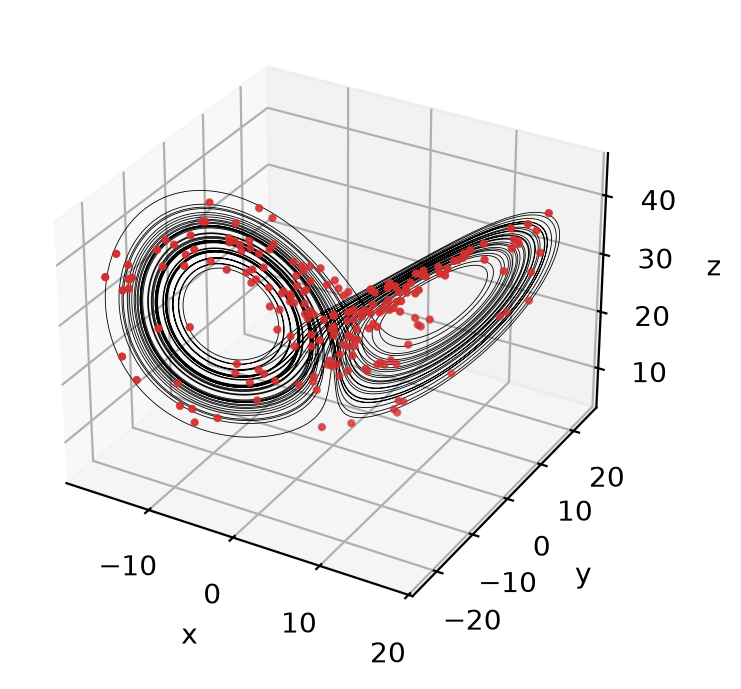
\includegraphics[width=0.55\linewidth]{figures/ch03-lorenz.png}
\caption{Output of \file{ch03_lorenz.py}: the Lorenz butterfly (black), and in red where 200 initial
conditions, all within $\sim10^{-3}$ of $\vb x_0$, are at $t=15$. They have spread over the whole
attractor (their range is $\sim35$--$45$ in each coordinate).}\label{fig:si-lorenz}
\end{nfigure}

\paragraph{Sensitive dependence.} Brunton closes with a movie of a small red blob of initial
conditions integrated through the system: it stretches, folds and mixes over the butterfly wings
\ts{3}{1}{13:55}\ts{3}{1}{14:15}. Any uncertainty in the initial condition grows exponentially; two points
starting very close end up far apart, and after long enough only a statistical description of where the
points are is possible \ts{3}{1}{14:36}. The red points of \cref{fig:si-lorenz} reproduce this.

% ------------------------------------------------------------------
\section{From continuous to discrete time}\label{sec:si-discrete}

A continuous-time system $\dot{\vb x}(t)=\vb f(\vb x(t))$ (the populations of a predator and a prey, or
anything else) \ts{3}{2}{0:01}\ts{3}{2}{0:22} induces a discrete-time system
$\vb x_{k+1}=\vb F(\vb x_k)$ \ts{3}{2}{1:03}. Usually $k$ is the step of an integrator, but it need not
be time at all \ts{3}{2}{1:23}. Sampling every $\Delta t$ (say, counting a population once a day),
$\vb x_k=\vb x(k\Delta t)$, and $\vb F$ is the flow map of \cref{def:fu-flowmap}
\ts{3}{2}{1:43}\ts{3}{2}{2:04}:
\begin{equation}\label{eq:si-flowmap}
  \vb x_{k+1}=\vb F_{\Delta t}(\vb x_k)=\vb x_k+\int_{k\Delta t}^{(k+1)\Delta t}\vb f(\vb x(\tau))\,\mathrm d\tau ,
\end{equation}
where the state inside the integral moves along the trajectory \ts{3}{2}{2:25}\ts{3}{2}{3:08}\ts{3}{2}{3:50}.

\begin{proposition}[Maps are more general than flows]
Every continuous-time system defines a discrete-time one through \eqref{eq:si-flowmap}, but not every
map is the flow map of some ODE \ts{3}{2}{4:10}\ts{3}{2}{4:32}.
\end{proposition}
Real populations, with seasons and other discrete events, are naturally maps \ts{3}{2}{4:52}. A
mathematical obstruction: a flow map $\vb F_{\Delta t}=\vb F_{\Delta t/2}\circ\vb F_{\Delta t/2}$ is a
diffeomorphism isotopic to the identity, so in one dimension it is increasing; the logistic map, which
is not invertible, cannot be the flow map of any one-dimensional ODE (a one-dimensional ODE cannot even
oscillate, let alone be chaotic).

\paragraph{Forward Euler as a crude flow map.} Replace the derivative by a finite difference
\ts{3}{2}{5:13}\ts{3}{2}{5:34}:
\[
  \frac{\vb x_{k+1}-\vb x_k}{\Delta t}\approx\vb f(\vb x_k)
  \quad\Longrightarrow\quad
  \vb x_{k+1}=\vb x_k+\Delta t\,\vb f(\vb x_k) .
\]
This is \eqref{eq:si-flowmap} with the integral approximated by a left rectangle: $\vb f$ held constant
over the step \ts{3}{2}{6:16}\ts{3}{2}{6:57}. Runge--Kutta schemes are better approximations of the same
true flow map \ts{3}{2}{7:38}. Only a handful of systems have a closed-form flow map, notably the linear
ones, $\vb F_t=e^{At}$; in general it must be approximated numerically \ts{3}{2}{7:59}.

\begin{proposition}[Order of Euler and RK4]\label{prop:si-order}
For smooth $\vb f$ the local error of one Euler step is $O(\Delta t^2)$ and the global error at a fixed
final time is $O(\Delta t)$; for the classical fourth-order Runge--Kutta scheme they are $O(\Delta t^5)$
and $O(\Delta t^4)$.
\end{proposition}
\begin{proof}
Taylor: $\vb x(t+\Delta t)=\vb x+\Delta t\,\vb f+\tfrac12\Delta t^2\,D\vb f\,\vb f+O(\Delta t^3)$; Euler
keeps the first two terms, so its local error is $\tfrac12\Delta t^2 D\vb f\,\vb f$. Over $N=T/\Delta t$
steps the local errors add up (each amplified at most by $e^{LT}$, $L$ the Lipschitz constant), giving
$N\cdot O(\Delta t^2)=O(\Delta t)$. RK4 matches the Taylor series up to $\Delta t^4$ (one checks it
term by term), hence local $O(\Delta t^5)$, global $O(\Delta t^4)$.
\end{proof}

\codefile{Euler and RK4 against the exact flow map}{../code/ch03_euler.py}

For the harmonic oscillator over one period the script prints, for $\Delta t\approx0.1,0.01,0.001$:
Euler errors $3.7\times10^{-1}$, $3.2\times10^{-2}$, $3.1\times10^{-3}$ (a factor 10 per factor 10 in
$\Delta t$: first order); RK4 errors $5.2\times10^{-6}$, $5.2\times10^{-10}$, $5.3\times10^{-14}$ (a
factor $10^4$: fourth order).

\begin{example}[Euler spirals outward]
For $\dot{\vb x}=A\vb x$ with $A=\begin{psmallmatrix}0&1\\-1&0\end{psmallmatrix}$ Euler gives
$\vb x_{k+1}=(I+\Delta tA)\vb x_k$, whose eigenvalues $1\pm i\Delta t$ have modulus
$\sqrt{1+\Delta t^2}>1$: the discrete orbit spirals out, energy grows by a factor
$(1+\Delta t^2)$ per step, while the true eigenvalues $e^{\pm i\Delta t}$ lie on the unit circle.
\end{example}

% ------------------------------------------------------------------
\section{The logistic map}\label{sec:si-logistic}

\paragraph{The model.} The logistic map
\begin{equation}\label{eq:si-logistic}
  x_{k+1}=\beta x_k(1-x_k)
\end{equation}
is a crude model of a population \ts{3}{2}{8:40}\ts{3}{3}{14:39}. Start from exponential growth,
$x_{k+1}=\beta x_k$; resources are finite, so with a carrying capacity normalized to 1 the growth factor
must go to zero as $x\to1$; multiplying by $(1-x_k)$ does that \ts{3}{3}{14:59}\ts{3}{3}{15:20}. It has
fixed points for zero and for ``full'' population, and as $\beta$ is turned up it becomes chaotic
\ts{3}{2}{9:01}\ts{3}{2}{9:22}.

\paragraph{The algorithm} \ts{3}{3}{1:03}\ts{3}{3}{1:45}:
\begin{enumerate}
  \item for each $\beta$ on a grid from $0$ to $4$, start from $x_0=0.5$;
  \item iterate a few thousand times without saving, to remove the transient and land on the attractor
        \ts{3}{3}{2:26}\ts{3}{3}{3:28};
  \item iterate up to a thousand more times, saving the pairs $(\beta,x_k)$; stop early if $x_k$ returns
        within $10^{-3}$ of the first saved value (a fixed point or a short periodic orbit needs no more
        points) \ts{3}{3}{3:49}\ts{3}{3}{4:52}\ts{3}{3}{5:12};
  \item scatter-plot all the pairs: the \emph{bifurcation diagram} \ts{3}{3}{5:54}.
\end{enumerate}

\codefile{bifurcation diagram of the logistic map}{../code/ch03_logistic.py}

\begin{coursenote}[Operator precedence]
In the video the update is written as ``\texttt{xold - xold\^{}2} times beta'', i.e.\
$(x-x^2)\beta=\beta x(1-x)$. Typed literally as \texttt{x - x**2*beta} it would be the map
$x-\beta x^2$, which is conjugate to the logistic map at fixed parameter 1 and never becomes chaotic
(and for $\beta>2$ leaves $[0,1]$ and diverges): a bug made, and caught, while writing these notes.
\end{coursenote}

\begin{nfigure}
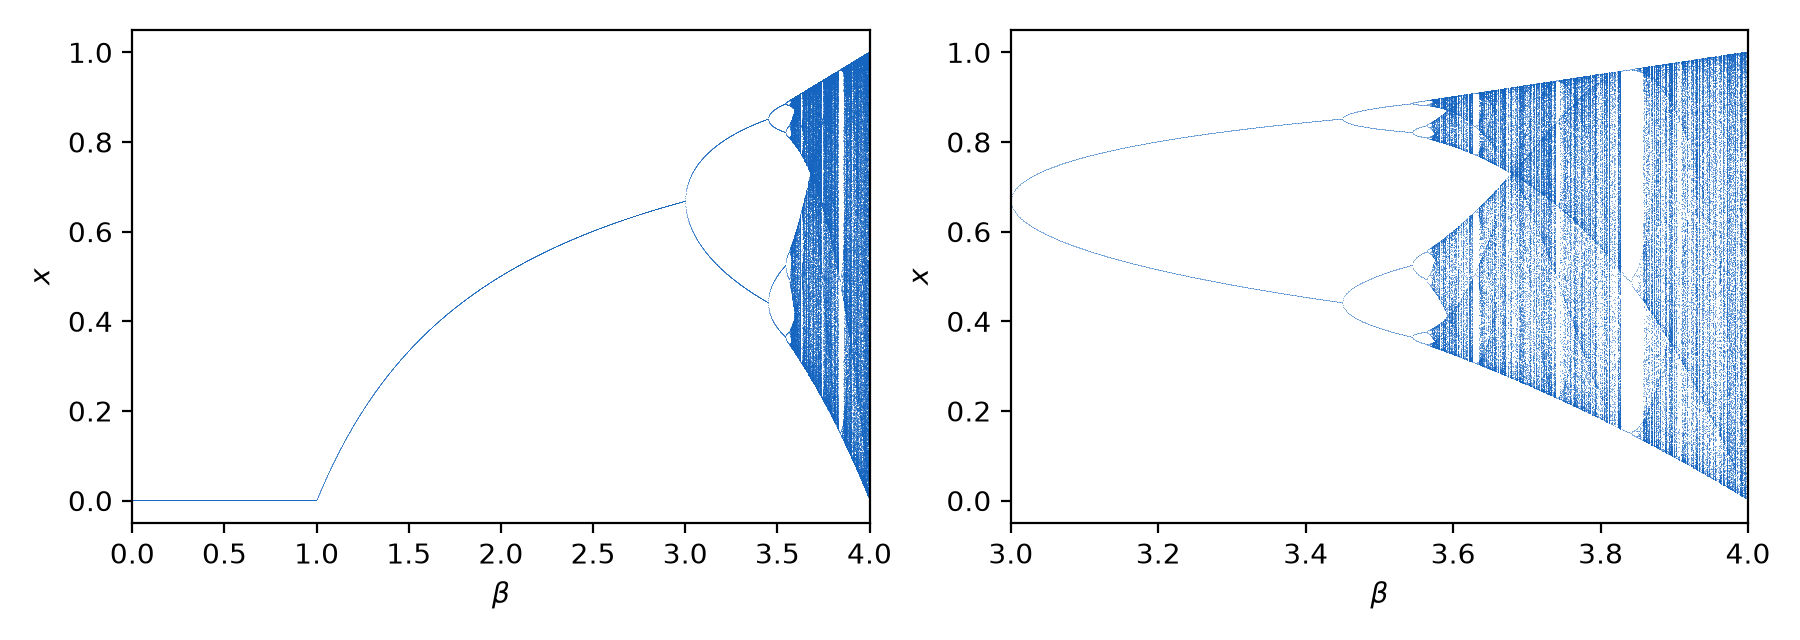
\includegraphics[width=\linewidth]{figures/ch03-logistic.png}
\caption{Output of \file{ch03_logistic.py}: bifurcation diagram of the logistic map (left, $\beta\in[0,4)$)
and zoom on $\beta\in[3,4]$ (right). In the video the axes are flipped so that the picture looks like
mountains, ``mathematical mountains'' \ts{3}{3}{8:43}\ts{3}{3}{13:57}.}\label{fig:si-logistic}
\end{nfigure}

\paragraph{Reading the diagram} \ts{3}{3}{7:20}:
\begin{itemize}
  \item $0\le\beta<1$: every orbit goes to $x=0$, the population dies out;
  \item $1<\beta<3$: a single nonzero fixed point, reached after a transient and kept forever
        \ts{3}{3}{7:40};
  \item at $\beta=3$ the fixed point splits into two values visited alternately, a period-2 orbit:
        the population is bigger, smaller, bigger, smaller from one generation to the next
        \ts{3}{3}{8:02};
  \item increasing $\beta$ the period doubles again, to 4 (Brunton calls it ``quasi periodic'', but it
        is a period-4 orbit), then 8, 16, \dots\ \ts{3}{3}{8:22};
  \item between about $3.57$ and $4$ the system is chaotic, with windows of periodic behaviour (the
        clear window near $\beta\approx3.83$ is a period-3 orbit) \ts{3}{3}{8:22}\ts{3}{3}{13:16}.
\end{itemize}
Keeping the transients in the plot shows the lines along which $x$ jumps from $0.5$ to the attractor
\ts{3}{3}{11:08}\ts{3}{3}{11:52}; that is why they are usually removed \ts{3}{3}{12:14}.

\begin{proposition}[First two bifurcations]\label{prop:si-logistic}
For \eqref{eq:si-logistic}, $F(x)=\beta x(1-x)$:
\begin{enumerate}[(i)]
  \item the fixed points are $x=0$ and $x^*=1-1/\beta$; $x=0$ is stable for $\beta<1$, and $x^*$ is
        stable for $1<\beta<3$;
  \item at $\beta=3$, $F'(x^*)=-1$ and a stable period-2 orbit is born (period-doubling, or
        \emph{flip}, bifurcation); it is stable for $3<\beta<1+\sqrt6\approx3.449$.
\end{enumerate}
\end{proposition}
\begin{proof}
A fixed point of a map is stable if $|F'(x^*)|<1$ (the linearization of $x_{k+1}=F(x_k)$ is
$\Delta x_{k+1}=F'(x^*)\Delta x_k$). $F'(x)=\beta(1-2x)$, so $F'(0)=\beta$ and
$F'(x^*)=\beta(1-2+2/\beta)=2-\beta$, with $|2-\beta|<1\iff1<\beta<3$. At $\beta=3$ the multiplier
crosses $-1$: deviations alternate in sign without decaying. The period-2 points solve $F(F(x))=x$; dividing
out the fixed points leaves $\beta^2x^2-\beta(\beta+1)x+(\beta+1)=0$, real for $\beta>3$; the multiplier of
the orbit is $F'(x_1)F'(x_2)=-\beta^2+2\beta+4$, which equals $-1$ at $\beta=1+\sqrt6$.
\end{proof}

\begin{intuition}[Faster growth, more chaos]
The moral Brunton draws from this crude model: the faster the growth rate, the more erratic the
population; ``breakneck population growth'' is a bad idea \ts{3}{3}{15:41}\ts{3}{3}{16:02}. The physical
reason is overshoot: with a large $\beta$ a big population produces a crash the next year, and the
discrete delay (one generation) turns a smooth relaxation into oscillations.
\end{intuition}

\begin{history}[May, Feigenbaum and universality]
The ecologist Robert May made the logistic map famous with \emph{Simple mathematical models with very
complicated dynamics}, Nature 261 (1976) 459--467, a plea to teach students that simple nonlinear maps
can be chaotic. Mitchell Feigenbaum (Los Alamos, 1975--78) found, at first with an HP-65 pocket
calculator, that the parameter values of successive period doublings converge geometrically with ratio
$\delta=4.6692\ldots$, the \emph{same} for every map with a quadratic maximum: a universal constant,
later explained by renormalization. Libchaber and Maurer saw the cascade in convecting liquid helium in
1980.\par
\textit{References:} R.~M.~May, Nature 261 (1976); M.~J.~Feigenbaum, J.\ Stat.\ Phys.\ 19 (1978) 25--52;
S.~Strogatz, \emph{Nonlinear Dynamics and Chaos}, ch.~10.
\end{history}

\begin{keyformulas}
\begin{itemize}
  \item Lorenz: $\dot x=\sigma(y-x)$, $\dot y=x(\rho-z)-y$, $\dot z=xy-\beta z$; $(10,28,8/3)$; $\vb x_0=(0,1,20)$.
  \item Flow map $\vb x_{k+1}=\vb x_k+\int_{k\Delta t}^{(k+1)\Delta t}\vb f(\vb x(\tau))\dd\tau$; Euler
        $\vb x_{k+1}=\vb x_k+\Delta t\vb f(\vb x_k)$, global error $O(\Delta t)$; RK4 $O(\Delta t^4)$.
  \item Logistic $x_{k+1}=\beta x_k(1-x_k)$: $x^*=1-1/\beta$ stable for $1<\beta<3$; period doubling at
        $3$, $1+\sqrt6$, \dots; chaos beyond $\approx3.57$.
\end{itemize}
\end{keyformulas}

\section*{Exercises}

\begin{exercise}[Lorenz fixed points]
Find the fixed points of \eqref{eq:si-lorenz} for $\rho>1$ and compute the Jacobian at the origin.
Show that the origin is stable for $\rho<1$ and a saddle with a one-dimensional unstable manifold for
$\rho>1$. Show that the volume of phase space contracts at the constant rate
$\nabla\cdot\vb f=-(\sigma+1+\beta)$, and conclude that the attractor has zero volume.
\end{exercise}

\begin{exercise}[Two nearby trajectories]
Modify \file{ch03_lorenz.py} to integrate $\vb x_0$ and $\vb x_0+10^{-8}(1,0,0)$, and plot
$\log\lVert\delta\vb x(t)\rVert$. Fit the slope of the linear part: compare with the largest Lyapunov
exponent $\lambda_1\approx0.906$. Why does the curve saturate?
\end{exercise}

\begin{exercise}[Tolerance matters]
Integrate Lorenz to $t=50$ with \texttt{rtol} $=10^{-3},10^{-6},10^{-9},10^{-12}$ and compare the final
states. Up to which time do the trajectories agree? Relate this to the prediction horizon of
Chapter~2.
\end{exercise}

\begin{exercise}[Backward Euler]
For $\dot{\vb x}=A\vb x$, backward Euler is $\vb x_{k+1}=(I-\Delta tA)^{-1}\vb x_k$. Compute its eigenvalues
for the harmonic oscillator and show that it spirals \emph{inward}. Which combination of forward and
backward Euler (the trapezoidal rule) preserves $|\mu|=1$ exactly?
\end{exercise}

\begin{exercise}[Period three]
Plot $F^3(x)-x$ for the logistic map near $\beta=1+\sqrt8\approx3.828$ and show that a pair of period-3
orbits is born there in a saddle-node (tangent) bifurcation. Run \file{ch03_logistic.py} zoomed on
$[3.82,3.86]$ and describe what happens at the edges of the window. (Li and Yorke, 1975: ``period
three implies chaos''.)
\end{exercise}

\begin{exercise}[Feigenbaum's constant]
Using bisection on the multiplier of the period-$2^n$ orbit, or by reading the zoomed bifurcation
diagram, estimate the first four period-doubling values $\beta_1=3$, $\beta_2\approx3.449$, $\beta_3$,
$\beta_4$, and the ratios $(\beta_n-\beta_{n-1})/(\beta_{n+1}-\beta_n)$.
\end{exercise}

\end{paracol}


\part{Learning models from data: regression}\label{part:regression}
% !TEX root = ../main.tex
\chapter{Dynamic Mode Decomposition}\label{ch:dmd}
\begin{paracol}{2}

\begin{sources}
\begin{tabularx}{\linewidth}{@{}V l L@{}}
\toprule
\textbf{Video} & \textbf{Length} & \textbf{Content}\\
\midrule
\seg{4}{1}{V4.1 Dynamic Mode Decomposition (Overview)} & 18:18 & Snapshot matrices $X$, $X'$; the best-fit linear operator $A$; the algorithm (SVD, $\tilde A$, eigendecomposition, exact modes); truncation; prediction; DMD = PCA in space + Fourier in time.\\
\seg{4}{2}{V4.2 Dynamic Mode Decomposition (Examples)} & 7:43 & Connection to Koopman; extensions (compressed, multiresolution, control, randomized, streaming, denoising, extended); applications; the toy video: PCA vs ICA vs DMD.\\
\seg{4}{3}{V4.3 Dynamic Mode Decomposition (Code)} & 8:15 & The cylinder-wake code of the DMD book: singular values, rank $r=21$, modes, eigenvalues on the unit circle.\\
\seg{4}{4}{V4.4 Compressed Sensing and Dynamic Mode Decomposition} & 30:35 & Compressed sensing; compressive-sampling DMD (L1 reconstruction of modes) and compressed DMD (modes from the full $X'$); error analysis; invariance of DMD under unitary transformations.\\
\bottomrule
\end{tabularx}

\smallskip
\textbf{Transcripts} \file{materials/transcripts/C04-V0*.txt}.
\textbf{Book} Sec.~7.2 (DMD); Sec.~1.4--1.5 (SVD, pseudo-inverse, PCA); Ch.~3 (compressed sensing).
\textbf{Code} \file{code/ch04_dmd.py}, \file{ch04_cdmd.py}. The cylinder data of the videos are not
used (they are on dmdbook.com); a toy data set reproduces the same effects.
\end{sources}

\section*{Motivation}
DMD is the first data-driven method of the course and the most widely used. From a movie of a
high-dimensional system it extracts, purely from data, (a) a few spatial patterns, the \emph{modes}, and
(b) for each one a single complex frequency, i.e.\ a pure oscillation with exponential growth or decay;
together they form a linear reduced-order model \ts{4}{1}{0:02}. It needs no equations of motion: ``turn
the crank'' on any time-resolved data \ts{4}{1}{1:26}. For a physicist: it is a numerically robust way
to find the normal modes of a system you can only film.

% ------------------------------------------------------------------
\section{The DMD algorithm}\label{sec:dmd-algorithm}

\paragraph{History and scope.} DMD was introduced in fluid dynamics by Peter Schmid and later connected
to Koopman operator theory by Clancy Rowley, Igor Mezi\'c and collaborators \ts{4}{1}{0:44}. Since then it
has been applied to disease modelling, neuroscience, robotics, finance, plasmas \ts{4}{1}{1:05}, and it
works equally on experimental data such as PIV images \ts{4}{1}{1:46}.

\begin{history}[Schmid, Rowley, Mezi\'c]
P.~J.~Schmid presented DMD in 2008 and published it as \emph{Dynamic mode decomposition of numerical and
experimental data}, J.\ Fluid Mech.\ 656 (2010) 5--28. C.~W.~Rowley, I.~Mezi\'c, S.~Bagheri,
P.~Schlatter and D.~S.~Henningson, \emph{Spectral analysis of nonlinear flows}, J.\ Fluid Mech.\ 641
(2009) 115--127, showed that DMD approximates the eigenvalues and modes of the Koopman operator,
building on Mezi\'c's \emph{Koopman modes} (2005). The ``exact DMD'' used today is from J.~H.~Tu,
C.~W.~Rowley, D.~M.~Luchtenburg, S.~L.~Brunton and J.~N.~Kutz, J.\ Comput.\ Dyn.\ 1 (2014) 391--421.\par
\textit{References:} the papers cited; Kutz, Brunton, Brunton, Proctor, \emph{Dynamic Mode
Decomposition} (SIAM, 2016).
\end{history}

\paragraph{Step 1: data.} Take a movie of the flow, e.g.\ vortex shedding behind a cylinder, cut it into
snapshots $\vb x_1,\dots,\vb x_m$ (each a vorticity field with $\sim10^5$ values, reshaped into a tall
column), and arrange them in two matrices shifted by one time step \ts{4}{1}{2:07}\ts{4}{1}{2:48}\ts{4}{1}{3:29}:
\begin{equation}\label{eq:dmd-data}
  X=\begin{bmatrix}\vb x_1&\vb x_2&\cdots&\vb x_{m-1}\end{bmatrix},\qquad
  X'=\begin{bmatrix}\vb x_2&\vb x_3&\cdots&\vb x_m\end{bmatrix}.
\end{equation}
For fluids these are very tall and skinny: $n\sim10^5$--$10^9$ rows, $m\sim10^2$--$10^3$ columns
\ts{4}{1}{4:10}.

\paragraph{Step 2: the hypothesis.} Look for the best-fit linear operator with \ts{4}{1}{4:31}\ts{4}{1}{4:51}
\begin{equation}\label{eq:dmd-A}
  X'\approx AX,\qquad A=\operatorname*{argmin}_A\lVert X'-AX\rVert_F=X'X^{\dagger},
\end{equation}
where $X^\dagger$ is the Moore--Penrose pseudo-inverse. This does not claim that the dynamics is linear
(Navier--Stokes is not): $A$ simply has enough freedom to approximate the evolution of the data
\ts{4}{4}{2:51}. But $A$ is $n\times n$, a trillion entries for $n=10^6$: it cannot even be stored
\ts{4}{1}{5:12}\ts{4}{1}{5:32}.

\begin{definition}[New concepts: DMD eigenvalues and modes]\label{def:dmd}
The \textbf{dynamic mode decomposition} of the data \eqref{eq:dmd-data} is the set of leading eigenvalues
$\lambda_j$ (\textbf{DMD eigenvalues}) and eigenvectors $\boldsymbol\phi_j$ (\textbf{DMD modes}) of
$A=X'X^\dagger$, computed without forming $A$ \ts{4}{1}{5:52}\ts{4}{1}{14:07}. Each mode, reshaped, is a
spatial pattern (an ``eigen flow field'') that evolves in time as $\lambda_j^k$: a pure tone, a pure
exponential growth or decay, or a growing or decaying oscillation \ts{4}{1}{6:13}\ts{4}{1}{6:33}.
\end{definition}

\paragraph{Step 3: the algorithm.} If enough snapshots are collected, a few coherent patterns dominate,
even with a million degrees of freedom \ts{4}{1}{7:56}\ts{4}{1}{8:17}. The algorithm exploits this
\ts{4}{1}{8:37}--\ts{4}{1}{12:23}:
\begin{enumerate}
  \item \textbf{SVD}: $X=U\Sigma V^*$ (economy size), truncated to rank $r$: $U_r\in\C^{n\times r}$,
        $\Sigma_r$, $V_r$. The columns of $U$ are the POD modes, ordered by the variance they capture
        \ts{4}{1}{8:37}\ts{4}{1}{8:57};
  \item \textbf{projected operator}: with $A\approx X'V_r\Sigma_r^{-1}U_r^*$,
        \begin{equation}\label{eq:dmd-Atilde}
          \tilde A=U_r^*AU_r=U_r^*X'V_r\Sigma_r^{-1}\in\C^{r\times r},
        \end{equation}
        the best-fit linear dynamics of the POD coefficients \ts{4}{1}{9:18}\ts{4}{1}{9:59}\ts{4}{1}{10:41};
  \item \textbf{eigendecomposition}: $\tilde AW=W\Lambda$; the eigenvalues of $\tilde A$ are the nonzero
        eigenvalues of $A$ \ts{4}{1}{11:02}\ts{4}{1}{11:22};
  \item \textbf{exact DMD modes} (Tu et al.\ 2014, slightly different from Schmid's $U_rW$):
        \begin{equation}\label{eq:dmd-Phi}
          \Phi=X'V_r\Sigma_r^{-1}W
        \end{equation}
        \ts{4}{1}{11:42}\ts{4}{1}{12:03}.
\end{enumerate}
That is all: four or five lines of code, fast and scalable \ts{4}{1}{12:44}.

\begin{proposition}[Why the algorithm works]\label{prop:dmd-exact}
Let $A=X'V_r\Sigma_r^{-1}U_r^*$ (the best fit restricted to the span of $U_r$), $\tilde A=U_r^*AU_r$, and
$\tilde A\vb w=\lambda\vb w$ with $\lambda\neq0$. Then $\boldsymbol\phi=X'V_r\Sigma_r^{-1}\vb w$ satisfies
$A\boldsymbol\phi=\lambda\boldsymbol\phi$, and $\boldsymbol\phi\neq0$.
\end{proposition}
\begin{proof}
Note $\tilde A=U_r^*X'V_r\Sigma_r^{-1}$, so $U_r^*\boldsymbol\phi=\tilde A\vb w=\lambda\vb w$. Then
$A\boldsymbol\phi=X'V_r\Sigma_r^{-1}(U_r^*\boldsymbol\phi)=\lambda X'V_r\Sigma_r^{-1}\vb w=\lambda\boldsymbol\phi$.
If $\boldsymbol\phi=0$ then $\lambda\vb w=U_r^*\boldsymbol\phi=0$, impossible. Conversely every eigenvector
of $A$ with $\lambda\ne0$ lies in the range of $X'V_r$, so this gives all nonzero eigenvalues.
\end{proof}

\begin{intuition}[Lifting back with the data]
The small eigenvector $\vb w$ lives in POD-coefficient space; \eqref{eq:dmd-Phi} lifts it back to the
full space by taking a linear combination of the \emph{shifted} snapshots, columns of $X'$
\ts{4}{4}{6:38}. Schmid's projected modes $U_r\vb w$ are the projection of $\boldsymbol\phi$ onto the POD
subspace; the two coincide when the columns of $X'$ lie in the span of $X$.
\end{intuition}

\paragraph{Truncation.} With $r=m-1$ (exact SVD) one gets $m-1$ eigenvalues and modes. If the first,
say, five POD modes capture 99\% of the energy, keep $r=5$: a $5\times5$ $\tilde A$, five eigenvalues,
five modes \ts{4}{1}{13:06}\ts{4}{1}{13:27}. The rank $r$ is the main knob of DMD \ts{4}{3}{3:28}.

\paragraph{Prediction.} With $b_j$ the amplitude of each mode in the initial condition (e.g.\
$\vb b=\Phi^\dagger\vb x_1$) \ts{4}{1}{14:28},
\begin{equation}\label{eq:dmd-pred}
  \vb x_{k+1}\approx\sum_{j=1}^r b_j\lambda_j^{k}\boldsymbol\phi_j,
  \qquad\text{or}\qquad
  \vb x(t)\approx\sum_j b_j e^{\omega_jt}\boldsymbol\phi_j,\ \ \omega_j=\frac{\ln\lambda_j}{\Delta t}.
\end{equation}
This works well for periodic or quasi-periodic systems, even strongly nonlinear ones; strong transients,
intermittency or non-stationarity need fancier regressions and a nonlinear framework \ts{4}{1}{14:49}\ts{4}{1}{15:09}.

\begin{remark}[DMD is regression]
The key observation (J.~Tu): DMD \emph{is} a best-fit linear regression from $X$ to $X'$, so every
regression technique applies: noise-robust regression, sparsity-promoting regression, and so on
\ts{4}{1}{15:30}\ts{4}{1}{15:50}.
\end{remark}

\begin{intuition}[PCA and Fourier ``had a baby'']
The SVD step is PCA: it finds the fewest patterns that explain the data. Then a linear regression on the
principal components ($\tilde A$) is diagonalized to find linear combinations of them that each have a
single frequency in time. DMD is PCA in space plus the Fourier transform in time \ts{4}{1}{16:11}\ts{4}{1}{16:52}\ts{4}{1}{17:13}.
Unlike a Fourier transform, the frequencies are not fixed by the record length and can grow or decay.
\end{intuition}

\begin{keyformulas}
\begin{itemize}
  \item $X'\approx AX$, $A=X'X^\dagger$; $X=U_r\Sigma_rV_r^*$; $\tilde A=U_r^*X'V_r\Sigma_r^{-1}$;
        $\tilde AW=W\Lambda$; $\Phi=X'V_r\Sigma_r^{-1}W$.
  \item $\vb x_k\approx\Phi\Lambda^{k-1}\vb b$, $\omega_j=\ln\lambda_j/\Delta t$: $\operatorname{Re}\omega_j$
        growth rate, $\operatorname{Im}\omega_j$ angular frequency.
\end{itemize}
\end{keyformulas}

% ------------------------------------------------------------------
\section{Extensions, applications, and a toy example}\label{sec:dmd-examples}

\paragraph{Connection to Koopman.} Although DMD fits a linear model, it is connected to strongly
nonlinear dynamics: its eigenvalues and modes approximate those of the Koopman operator (Chapter~6)
\ts{4}{2}{0:23}\ts{4}{2}{0:44}.

\paragraph{Extensions.} Because DMD is linear regression, it is easily extended \ts{4}{2}{1:05}:
\begin{itemize}
  \item \textbf{compressed / compressed-sensing DMD}, for spatially under-resolved data, and compressed
        sensing in time for data that are not time resolved (\cref{sec:dmd-cs}) \ts{4}{2}{1:26};
  \item \textbf{multiresolution DMD} (N.~Kutz): DMD on a hierarchy of time windows, separating slow,
        medium and fast modes; it captures transient phenomena such as El Ni\~no \ts{4}{2}{1:46};
  \item \textbf{DMD with control} (J.~Proctor): identify the model while the system is actuated,
        $\vb x_{k+1}\approx A\vb x_k+B\vb u_k$ \ts{4}{2}{2:07};
  \item \textbf{randomized DMD} (N.~B.~Erichson and others) for very large data \ts{4}{2}{2:28};
  \item \textbf{streaming}, \textbf{denoising} and \textbf{extended} DMD (augmenting the measurements with
        nonlinear functions of them) \ts{4}{2}{2:48}\ts{4}{2}{3:09}.
\end{itemize}
Literally dozens of papers add innovations to the original algorithm \ts{4}{2}{3:29}.

\begin{application}[Where DMD is used]
Most DMD papers are in fluid dynamics (a jet in cross flow by Rowley, Mezi\'c et al., boundary layers,
combustion, shock--boundary-layer interaction), but also neuroscience, disease modelling, weather and
climate, robotics, finance, plasmas and video processing \ts{4}{2}{3:50}\ts{4}{2}{4:10}. The common
thread: high-dimensional data from a probably nonlinear, multiscale process with dominant coherent
structures \ts{4}{2}{4:31}.
\end{application}

\begin{casestudy}[A toy video: PCA, ICA and DMD]
B.~W.~Brunton's toy movie: $80\times80$ pixels (6400-dimensional data), with noise, in which two patterns
oscillate at different frequencies, a fast square and a slow Gaussian; without noise it is a rank-2
system \ts{4}{2}{4:51}\ts{4}{2}{5:12}\ts{4}{2}{5:33}.
\begin{itemize}
  \item \textbf{PCA} (the SVD) gets the rank right, 2, but its modes, ordered by energy, \emph{mix} the
        two frequencies \ts{4}{2}{5:53}\ts{4}{2}{6:14};
  \item \textbf{ICA} extracts two shapes corresponding to fast and slow, but they are noisy and there is no
        model of their time evolution \ts{4}{2}{6:35};
  \item \textbf{DMD} separates square and Gaussian cleanly, denoises them, and identifies the two
        frequencies: a linear dynamical model is under the hood \ts{4}{2}{6:55}\ts{4}{2}{7:15}.
\end{itemize}
\end{casestudy}

\codefile{DMD function and the toy video}{../code/ch04_dmd.py}

\begin{nfigure}
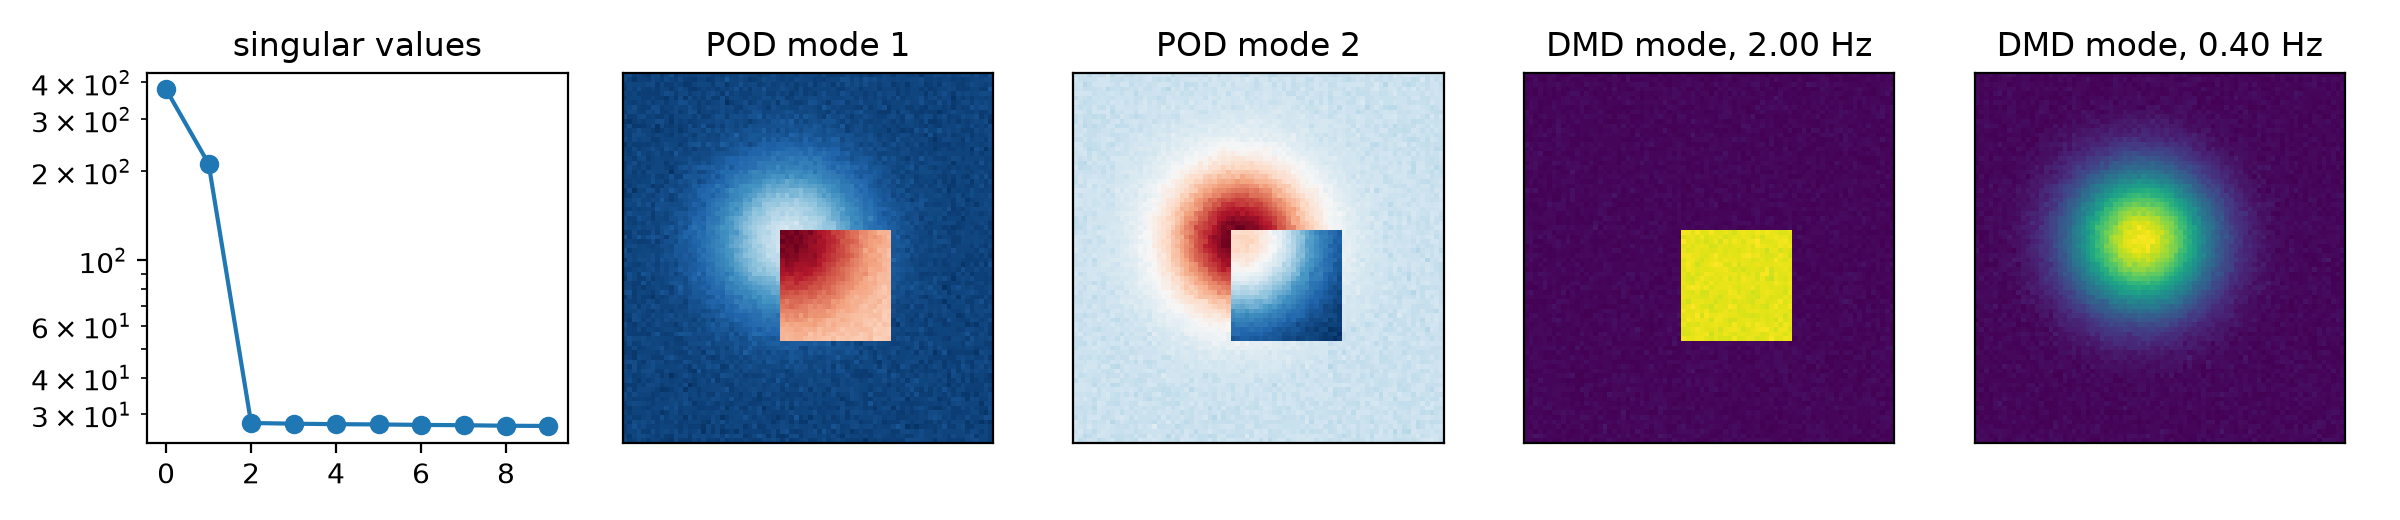
\includegraphics[width=\linewidth]{figures/ch04-dmd-toy.png}
\caption{Output of \file{ch04_dmd.py}. Singular values: rank 2 plus a noise floor. POD modes 1--2 mix
the square and the Gaussian (which overlap and are not orthogonal); the two DMD modes (modulus) separate
them, with the right frequencies, 2.00 and 0.40\,Hz, and growth rates $\approx0$ (the script prints
$-0.003$ and $-0.008\,\mathrm{s}^{-1}$, a small bias due to the noise).}\label{fig:dmd-toy}
\end{nfigure}

\begin{remark}[Noise bias]
With noise, DMD eigenvalues are biased towards the inside of the unit circle (spurious damping), because
least squares attributes all the noise to $X'$ and none to $X$. Remedies are noise-robust regressions:
forward--backward DMD, total-least-squares DMD, optimized DMD.
\end{remark}

% ------------------------------------------------------------------
\section{DMD in practice: the cylinder wake}\label{sec:dmd-code}

The code of the DMD book (dmdbook.com) for the flow past a cylinder \ts{4}{3}{0:22}\ts{4}{3}{1:04}:
\begin{enumerate}
  \item load the vorticity fields, one per column, and split them into $X$ (columns $1..m-1$) and $X'$
        (columns $2..m$) \ts{4}{3}{1:24}\ts{4}{3}{1:45};
  \item economy SVD of $X$ (a full SVD would be far too expensive) \ts{4}{3}{2:05};
  \item plot the singular values on a log scale, always a good idea \ts{4}{3}{2:05}: the first one is the
        mean flow (not subtracted), then they come in \emph{pairs}, the sine/cosine pairs of the periodic
        shedding and its harmonics \ts{4}{3}{2:47}\ts{4}{3}{3:08};
  \item truncate at $r=21$: the mean plus ten harmonic pairs \ts{4}{3}{3:28}\ts{4}{3}{3:48};
  \item compute $\tilde A$ ($21\times21$), its eigendecomposition and the modes $\Phi$, ``three lines''
        \ts{4}{3}{4:09}\ts{4}{3}{4:50}\ts{4}{3}{6:33};
  \item plot the modes: pairs oscillating at one frequency, finer and finer for higher harmonics
        \ts{4}{3}{5:32}\ts{4}{3}{5:52};
  \item plot the eigenvalues with the unit circle (discrete time): complex-conjugate pairs on the circle,
        which explains the sine/cosine pairs of modes oscillating out of phase \ts{4}{3}{6:53}\ts{4}{3}{7:14}.
\end{enumerate}
Here the DMD modes look much like the POD modes because the cylinder wake is a ``very normal'' system
\ts{4}{3}{5:52}\ts{4}{3}{6:12}.

\begin{secondary}[Why the modes come in pairs, and why DMD $\approx$ POD here]
A real travelling or rotating pattern $\operatorname{Re}(\boldsymbol\phi e^{i\omega t})=
\boldsymbol\phi_R\cos\omega t-\boldsymbol\phi_I\sin\omega t$ needs two real spatial fields, hence two
singular values of similar size and a conjugate pair $\lambda,\bar\lambda$. On the periodic attractor the
time coefficients of different harmonics are orthogonal over a period, so the SVD, which produces
orthogonal time series, cannot mix different frequencies, and the POD modes coincide (pairwise) with the
DMD modes. When the dynamics is non-normal or transient this fails, and DMD and POD differ.
\end{secondary}

% ------------------------------------------------------------------
\section{Compressed sensing and DMD}\label{sec:dmd-cs}

DMD needs a lot of data: acquiring and processing $X$, $X'$ can be expensive \ts{4}{4}{9:42}\ts{4}{4}{10:03}.
In PIV, for example, spatial and temporal resolution are limited by hardware: sometimes the data cannot
even be transferred from the camera to memory fast enough \ts{4}{4}{10:23}\ts{4}{4}{10:44}. Other uses of
sparsity in DMD: selecting few important modes (Jovanovi\'c et al.), sparse sampling in time (Tu et al.)
\ts{4}{4}{11:04}\ts{4}{4}{11:25}. Here: sparse sampling in \emph{space} \ts{4}{4}{11:46}.

\paragraph{Compressed sensing in one paragraph.} Most high-dimensional signals (images, flow fields,
audio) are \emph{sparse} in a suitable basis: in the Fourier domain most coefficients of an image are small
and can be dropped, which is how compression works \ts{4}{4}{12:06}\ts{4}{4}{12:27}\ts{4}{4}{12:48}.
Compressed sensing (about ten years old at the time of the video) turns this around: measure much less
and infer the sparse coefficients consistent with the measurements \ts{4}{4}{13:09}\ts{4}{4}{13:30}.

\begin{definition}[New concepts: sparsity, compressed sensing]\label{def:dmd-cs}
A vector $\vb x\in\R^n$ is $K$-\textbf{sparse} in a basis $\Psi$ if $\vb x=\Psi\vb s$ with at most $K$
nonzero entries in $\vb s$. Given $p\ll n$ measurements $\vb y=C\vb x=C\Psi\vb s$,
\textbf{compressed sensing} recovers $\vb s$ by the convex problem
\begin{equation}\label{eq:dmd-l1}
  \min_{\vb s}\lVert\vb s\rVert_1\quad\text{subject to}\quad\vb y=C\Psi\vb s
\end{equation}
instead of the combinatorial search for the sparsest $\vb s$ ($\ell_0$). It succeeds with high probability
if $p\gtrsim K\log(n/K)$ and the measurements are \emph{incoherent} with $\Psi$ (e.g.\ random), so that
$C\Psi$ satisfies the restricted isometry property: it acts almost like an isometry on sparse vectors
\ts{4}{4}{13:51}\ts{4}{4}{14:32}\ts{4}{4}{14:52}\ts{4}{4}{15:13}.
\end{definition}

The $\ell_1$ problem is a linear program: its cost grows polynomially, so Moore's law lets it keep up with
bigger data, which a brute-force search cannot \ts{4}{4}{15:13}\ts{4}{4}{15:33}. Example: measure 1\% of the
velocities of a flow at random points, infer its sparse Fourier coefficients, and fill in the other 99\%
\ts{4}{4}{16:15}\ts{4}{4}{16:36}.

\begin{history}[Compressed sensing]
Compressed sensing was founded in 2004--2006 by E.~Cand\`es, J.~Romberg and T.~Tao (\emph{Robust
uncertainty principles}, IEEE Trans.\ Inf.\ Theory 52, 2006) and D.~Donoho (\emph{Compressed sensing},
same journal and year). An early inspiration: Cand\`es reconstructed a Shepp--Logan phantom image almost
exactly from very few Fourier samples using $\ell_1$ (total-variation) minimization. The figure used in the
video is from R.~Baraniuk, \emph{Compressive sensing}, IEEE Signal Process.\ Mag.\ (2007).\par
\textit{References:} the papers cited; Brunton \& Kutz, Ch.~3.
\end{history}

\paragraph{Two algorithms.} With a measurement matrix $C\in\R^{p\times n}$ (e.g.\ random pixels), the
compressed data are $Y=CX$, $Y'=CX'$ \ts{4}{4}{17:39}\ts{4}{4}{17:59}.
\begin{enumerate}
  \item \textbf{Compressive-sampling (compressed-sensing) DMD}: only $Y,Y'$ exist (sparse sensors, or
        trading spatial for temporal resolution). Do DMD on $Y,Y'$, getting $\Lambda_Y$, $\Phi_Y$, then
        reconstruct each full mode by \eqref{eq:dmd-l1} with $\boldsymbol\phi_Y=C\Psi\vb s$
        \ts{4}{4}{18:20}. On the cylinder, $\sim1000$ measurements of a $\sim10^5$-dimensional state (1\%)
        reconstruct the leading modes well and the higher ones with some noise; the eigenvalues are almost
        exact, $\Lambda_X\approx\Lambda_Y$ to near machine precision \ts{4}{4}{18:41}\ts{4}{4}{19:01}.
  \item \textbf{Compressed DMD}: the full data exist but the SVD is too expensive. Compress, do DMD on
        $Y,Y'$, and get the full modes with no $\ell_1$ at all, as
        \begin{equation}\label{eq:dmd-cdmd}
          \Phi_X\approx X'V_Y\Sigma_Y^{-1}W_Y ,
        \end{equation}
        linear combinations of the columns of the full $X'$ \ts{4}{4}{19:43}\ts{4}{4}{20:24}. On the cylinder
        21 random pixels already give the first mode, 40 give all of them \ts{4}{4}{20:45}; cluster-sized
        computations fit on a laptop \ts{4}{4}{21:25}.
\end{enumerate}
The decision: only subsampled data $\Rightarrow$ compressive-sampling DMD with $\ell_1$; full data but slow
$\Rightarrow$ compressed DMD \ts{4}{4}{21:47}\ts{4}{4}{22:28}. With enough buoys in the ocean one could
infer the DMD of a high-resolution sensor network \ts{4}{4}{23:09}. In the error analysis on a double-gyre
flow, the mode error of compressed-sensing DMD decreases slowly (low at $\sim1000$ measurements, 1\%),
that of compressed DMD much faster (very good at $\sim100$) \ts{4}{4}{23:29}\ts{4}{4}{24:10}\ts{4}{4}{24:31}.

\codefile{compressed DMD on the toy video}{../code/ch04_cdmd.py}

The script prints, for $p=20,100,400$ random pixels out of 6400: eigenvalue errors $0.9$,
$1.4\times10^{-2}$, $5\times10^{-3}$ and mode errors $(0.41,0.16)$, $(0.02,0.01)$, $(0.008,0.005)$. With 20
pixels too few of them fall on the square and the Gaussian, which are \emph{localized}: in the pixel basis
these signals are not incoherent with point measurements. 100 pixels (1.6\%) are enough.

\paragraph{Why it works.} Three facts \ts{4}{4}{24:51}:
\begin{enumerate}
  \item DMD is invariant under \emph{right} unitary transformations: shuffling the columns of $X$ and of
        $X'$ in the same way gives the same eigenvalues and modes, because the SVD is invariant
        \ts{4}{4}{25:12}\ts{4}{4}{25:33};
  \item DMD is almost invariant under \emph{left} unitary transformations: if $Y=CX$, $Y'=CX'$ with $C$
        unitary (permuting rows, a spatial FFT, a POD basis), the eigenvalues are the same and the modes are
        $\Phi_Y=C\Phi_X$ \ts{4}{4}{25:53}\ts{4}{4}{26:13}\ts{4}{4}{26:34}\ts{4}{4}{26:54};
  \item a compression $C\in\R^{p\times n}$ is not unitary, but if the data are sparse, $X=\Psi S$, compressed
        sensing gives conditions under which $C\Psi$ acts like an isometry on sparse vectors, which is
        all that is needed \ts{4}{4}{27:35}\ts{4}{4}{27:56}\ts{4}{4}{28:17}\ts{4}{4}{28:59}.
\end{enumerate}

\begin{proof}[Proof of fact 2]
If $Y=CX$ with $C^*C=I$, then $Y=(CU)\Sigma V^*$ is an SVD of $Y$, so $U_Y=CU$, $\Sigma_Y=\Sigma$, $V_Y=V$.
Then $\tilde A_Y=U^*C^*CX'V\Sigma^{-1}=\tilde A_X$, so same $\Lambda$ and $W$, and
$\Phi_Y=CX'V\Sigma^{-1}W=C\Phi_X$.
\end{proof}

The code of the paper (a sparse dynamical system on a torus driving five spatial Fourier coefficients) is
available to try different compression ratios and samplings \ts{4}{4}{29:20}\ts{4}{4}{29:40}.

\section*{Exercises}

\begin{exercise}[DMD of a linear system]
Generate data from $\vb x_{k+1}=A\vb x_k$ with a random $A\in\R^{50\times50}$ of rank 4 (scaled so that its
eigenvalues have modulus $\le1$). Show numerically that DMD with $r=4$ recovers the nonzero eigenvalues of
$A$ exactly. What happens with $r=6$? With noise?
\end{exercise}

\begin{exercise}[Pseudo-inverse]
Show that $A=X'X^\dagger$ minimizes $\lVert X'-AX\rVert_F$, and that among the minimizers it has the smallest
Frobenius norm. Write $X^\dagger$ via the SVD.
\end{exercise}

\begin{exercise}[One real oscillation needs two modes]
Take data $x(t)=\cos(\omega t)\,\vb f$ for a fixed spatial vector $\vb f$. What is the rank of $X$? Can
DMD find the frequency? Now take $\vb f\cos\omega t+\vb g\sin\omega t$ with $\vb f\perp\vb g$: show that
$r=2$ gives $\lambda=e^{\pm i\omega\Delta t}$. Relate this to the singular-value pairs of the cylinder.
(This is the reason \file{ch04_dmd.py} uses complex data; Chapter~8 gives another cure: time delays.)
\end{exercise}

\begin{exercise}[Mean subtraction]
Run DMD on the toy data plus a constant background. Show that the mean appears as a mode with
$\lambda=1$. What happens to DMD if the mean is subtracted first? (Hint: Chen, Tu, Rowley 2012 show that
mean-subtracted DMD reduces to a temporal DFT.)
\end{exercise}

\begin{exercise}[Left-unitary invariance]
Verify fact 2 numerically on the toy data with $C$ the 2D FFT (normalized) and with a random orthogonal
$C$. Then try a random Gaussian $C\in\R^{p\times6400}$ and plot the eigenvalue error versus $p$.
\end{exercise}

\end{paracol}

% !TEX root = ../main.tex
\chapter{Sparse Identification of Nonlinear Dynamics}\label{ch:sindy}
\begin{paracol}{2}

\begin{sources}
\begin{tabularx}{\linewidth}{@{}V l L@{}}
\toprule
\textbf{Video} & \textbf{Length} & \textbf{Content}\\
\midrule
\seg{5}{1}{V5.1 Sparse Identification of Nonlinear Dynamics (SINDy)} & 26:44 & The SINDy regression on Lorenz; noisy data and TV derivatives; the cylinder wake and the mean-field model (history from Ruelle--Takens to Noack); kicking off the attractor; parametrized, time-dependent and forced models; SINDy in delay coordinates; SINDy with control; open questions.\\
\seg{5}{2}{V5.2 PDE FIND} & 10:36 & (Speaker: Samuel Rudy; uploaded by N.~Kutz.) Discovering PDEs $u_t=N(u,u_x,\dots)$ by sparse regression; derivatives; sequential threshold ridge regression; Navier--Stokes from 1\% of the data; the soliton ambiguity (advection vs KdV); a gallery of PDEs.\\
\bottomrule
\end{tabularx}

\smallskip
\textbf{Transcripts} \file{materials/transcripts/C05-V0*.txt}.
\textbf{Book} Sec.~7.3 (SINDy); Sec.~3.5 (sparse regression); Sec.~4.4--4.7 (regression, model selection).
\textbf{Papers} S.~L.~Brunton, J.~L.~Proctor, J.~N.~Kutz, PNAS 113 (2016) 3932--3937; S.~H.~Rudy,
S.~L.~Brunton, J.~L.~Proctor, J.~N.~Kutz, Sci.\ Adv.\ 3 (2017) e1602614.
\textbf{Code} \file{code/ch05_sindy.py}, \file{ch05_pdefind.py}.
\end{sources}

\section*{Motivation}
DMD (\cref{ch:dmd}) fits a \emph{linear} model to data. SINDy goes after the second primary challenge of
\cref{ch:overview}, unknown dynamics, head on: it discovers the nonlinear right-hand side $\vb f$ itself,
as a short formula, from measurements \ts{5}{1}{0:04}. If we had $\vb f$ we could integrate trajectories,
compute coherent structures and FTLEs, quantify uncertainty \ts{5}{1}{0:45}\ts{5}{1}{1:06}; in neuroscience or
climate science we do not have it, so we want to discover it from data \ts{5}{1}{1:27}. The key assumption is
\emph{parsimony}: in the right coordinates, $\vb f$ has only a few terms.

% ------------------------------------------------------------------
\section{The SINDy algorithm}\label{sec:si-algorithm}

\paragraph{Sparsity in function space.} In the Lorenz equations \eqref{eq:si-lorenz} the $\dot x$ equation
contains only $x$ and $y$; $\dot y$ contains $x$, $xz$ and $y$; $\dot z$ contains $z$ and $xy$
\ts{5}{1}{1:49}\ts{5}{1}{2:09}. Out of all possible right-hand sides this one is very special: it is
\emph{sparse} in the space of candidate functions \ts{5}{1}{2:30}\ts{5}{1}{3:11}.

\begin{definition}[New concepts: library, SINDy]\label{def:sindy}
From $m$ samples of the state and its derivative, build
\[
  X=\begin{bmatrix}\vb x^{\mathsf T}(t_1)\\\vdots\\\vb x^{\mathsf T}(t_m)\end{bmatrix}\in\R^{m\times n},\qquad
  \dot X\in\R^{m\times n},
\]
and a \textbf{library} of candidate functions evaluated on the data,
$\Theta(X)=\begin{bmatrix}\vb 1 & X & X^{P_2} & X^{P_3}&\cdots\end{bmatrix}$, where $X^{P_2}$ holds all
quadratic monomials ($x^2,xy,xz,y^2,\dots$), and so on \ts{5}{1}{3:32}. \textbf{SINDy} (Sparse
Identification of Nonlinear DYnamics) solves
\begin{equation}\label{eq:sindy}
  \dot X\approx\Theta(X)\,\Xi,\qquad \Xi=[\boldsymbol\xi_1\cdots\boldsymbol\xi_n]\ \text{sparse},
\end{equation}
one sparse regression per state variable: $\dot{\vb x}_k\approx\Theta(X)\boldsymbol\xi_k$ \ts{5}{1}{3:52}\ts{5}{1}{4:12}.
The identified model is $\dot x_k=\boldsymbol\theta(\vb x^{\mathsf T})\boldsymbol\xi_k$, with
$\boldsymbol\theta$ the row of library functions.
\end{definition}

\paragraph{Why sparse regression.} Plain least squares would use ``a little bit of all'' the columns
\ts{5}{1}{5:34}; an $\ell_1$-penalized (or thresholded) regression finds a good fit with as few terms as
possible \ts{5}{1}{5:56}. Options: the LASSO of Tibshirani, or the \emph{sequentially thresholded least
squares} of the paper \ts{5}{1}{4:53}.

\begin{definition}[New concepts: LASSO, sequentially thresholded least squares]
\begin{enumerate}[(a)]
  \item \textbf{LASSO} (Least Absolute Shrinkage and Selection Operator, Tibshirani 1996):
        $\min_{\boldsymbol\xi}\lVert\dot{\vb x}-\Theta\boldsymbol\xi\rVert_2^2+\alpha\lVert\boldsymbol\xi\rVert_1$.
  \item \textbf{STLSQ}: solve least squares; set to zero every coefficient with
        $|\xi_i|<\lambda$; solve least squares again on the surviving columns; repeat until the support
        stops changing. The threshold $\lambda$ is the sparsity knob.
\end{enumerate}
\end{definition}

\codefile{SINDy on the Lorenz system}{../code/ch05_sindy.py}

The script, with derivatives computed from the data by finite differences and a library of all 56
monomials up to order 5, prints
\[
  \dot x=-10.000x+10.000y,\quad \dot y=27.998x-1.000y-1.000xz,\quad \dot z=-2.667z+1.000xy ,
\]
the Lorenz system with its parameters; least squares would have kept 133 of the 168 coefficients. As in
the video: same structure, virtually the same $\sigma,\rho,\beta$, same dynamics on the attractor
\ts{5}{1}{6:16}.

\begin{intuition}[Occam's razor as an optimization]
The threshold implements a Pareto trade-off between accuracy and complexity: as $\lambda$ grows, terms
drop out; the right model sits at the ``knee'', where removing one more term makes the error jump. Choosing
$\lambda$ is model selection (cross-validation, information criteria such as AIC; book Sec.~4.6--4.7).
\end{intuition}

\paragraph{Noise and derivatives.} One rarely measures $\dot{\vb x}$; it must be computed from $\vb x$
\ts{5}{1}{6:58}. With very noisy measurements of $x,y,z$, \emph{total-variation regularized} derivatives
(TVDiff, R.~Chartrand) still allow correct structure identification and an accurate reconstruction of the
attractor \ts{5}{1}{7:18}\ts{5}{1}{7:39}; both steps are numerically robust \ts{5}{1}{7:59}.

\begin{secondary}[Total-variation regularized differentiation]
Find $u\approx\dot f$ as $\min_u\ \alpha\int|u'|\,\mathrm dt+\tfrac12\int\big|\!\int_0^tu-f\big|^2\mathrm dt$:
the integral of the derivative must reproduce the signal, while the total variation of the derivative is
penalized. Unlike finite differences, which amplify noise by $1/\Delta t$, this gives piecewise-smooth
derivatives. Alternatives: Savitzky--Golay filters, local polynomial fits (as in PDE-FIND), or the weak
(integral) form of SINDy, which avoids derivatives altogether.
\end{secondary}

\begin{exercise}[Noise and threshold]
Add Gaussian noise of standard deviation $\eta$ to $X$ in \file{ch05_sindy.py} before differentiating.
For $\eta=0.01,0.1,1$, find the range of $\lambda$ for which the correct structure is found. Replace the
finite differences by a Savitzky--Golay filter (\texttt{scipy.signal.savgol\_filter} with \texttt{deriv=1})
and compare.
\end{exercise}

% ------------------------------------------------------------------
\section{The cylinder wake: rediscovering the mean-field model}\label{sec:si-cylinder}

\begin{casestudy}[Thirty years in a regression]
A benchmark of fluid dynamics: flow past a cylinder, with vortex shedding \ts{5}{1}{8:20}. A low-order model
for it took decades \ts{5}{1}{8:40}:
\begin{enumerate}
  \item Ruelle and Takens (1971), after Landau and Hopf, proposed a route to turbulence through successive
        Hopf bifurcations \ts{5}{1}{9:00}\ts{5}{1}{9:21};
  \item about 15 years later, Zebib, Jackson and others verified numerically that the cylinder wake
        undergoes a Hopf bifurcation at Reynolds number $\approx47$, after which laminar periodic shedding
        sets in \ts{5}{1}{9:42}\ts{5}{1}{10:02};
  \item a paradox: the Hopf normal form \eqref{eq:fu-hopf} has \emph{cubic} terms, but Navier--Stokes has
        only \emph{quadratic} nonlinearity (convection) \ts{5}{1}{10:23}\ts{5}{1}{10:43};
  \item 15 years later again, Noack et al.\ (J.\ Fluid Mech.\ 2003) resolved it with a separation of time
        scales: the \emph{mean-field model}
        \begin{equation}\label{eq:si-meanfield}
          \dot x=\mu x-\omega y+Axz,\qquad \dot y=\omega x+\mu y+Ayz,\qquad \dot z=-\lambda(z-x^2-y^2),
        \end{equation}
        where $x,y$ are the amplitudes of the two shedding modes and $z$ the ``shift mode'' between the
        unstable steady flow and the mean flow. $z$ is fast: it collapses onto the slow parabolic manifold
        $z=x^2+y^2$, on which the dynamics winds out to periodic shedding \ts{5}{1}{11:04}\ts{5}{1}{11:24}\ts{5}{1}{11:46}.
        Only quadratic terms, yet a Hopf bifurcation \ts{5}{1}{12:06}.
\end{enumerate}
SINDy, fed the time series of the first two POD modes and the shift mode from a simulation, identifies a
model with the same structure: only quadratic terms, the slow parabolic manifold, the spiral onto shedding
\ts{5}{1}{12:27}\ts{5}{1}{12:48}\ts{5}{1}{13:10}.
\end{casestudy}

\begin{proposition}[Cubic from quadratic]
On the slow manifold $z=x^2+y^2$, model \eqref{eq:si-meanfield} reduces to the Hopf normal form
$\dot r=\mu r+Ar^3$ (supercritical for $A<0$), $\dot\theta=\omega$.
\end{proposition}
\begin{proof}
With $r^2=x^2+y^2$: $r\dot r=x\dot x+y\dot y=\mu r^2+Ar^2z$, so $\dot r=\mu r+Arz$; substituting $z=r^2$
gives $\dot r=\mu r+Ar^3$. Also $r^2\dot\theta=x\dot y-y\dot x=\omega r^2$. The cubic term is generated by
eliminating the fast variable: adiabatic elimination.
\end{proof}

\paragraph{Kick it off the attractor.} If the data start on the slow manifold, SINDy wrongly identifies
\emph{cubic} terms (the reduced model of the proposition) \ts{5}{1}{13:51}. To get the quadratic model one
must start off the attractor, e.g.\ from the mean flow, and watch the system fall back \ts{5}{1}{14:12}.
General strategy: to identify the dynamics near an attractor, kick the system off it and see how it
returns \ts{5}{1}{14:32}.

\begin{exercise}[Mean-field model]
Simulate \eqref{eq:si-meanfield} with $\mu=0.1$, $\omega=1$, $A=-0.1$, $\lambda=10$ from an initial
condition on the slow manifold, and from one off it ($z$ far from $x^2+y^2$). Run SINDy with polynomials up
to order 3 on both data sets: which one gives the quadratic model, which one the cubic normal form?
\end{exercise}

% ------------------------------------------------------------------
\section{Extensions: parameters, forcing, delays, control}\label{sec:si-extensions}

\paragraph{Parametrized dynamics ``for free''.} Treat a parameter $\mu$ as an extra state with
$\dot\mu=0$ and include it in the library ($\mu,\mu x,\mu x^2,\dots$) \ts{5}{1}{14:53}\ts{5}{1}{15:35}. For the
logistic map, training on 10 values of $\mu$ yields a parametrized model that reproduces the whole
bifurcation diagram \ts{5}{1}{15:14}\ts{5}{1}{15:56}; likewise for the Hopf normal form \ts{5}{1}{15:56}. In the same
way one can add time ($\sin t$, $t^2$, \dots) for non-autonomous systems, or external forcing such as CO$_2$
in a climate model \ts{5}{1}{16:16}\ts{5}{1}{16:36}.

\paragraph{Delay coordinates.} What if only $x$ of the Lorenz system is measured \ts{5}{1}{16:58}\ts{5}{1}{17:18}?
Build the \emph{Hankel matrix} of shifted copies of the time series \ts{5}{1}{17:39}\ts{5}{1}{18:00},
\begin{equation}\label{eq:si-hankel}
  H=\begin{bmatrix}x_1&x_2&\cdots&x_{m-p+1}\\ x_2&x_3&\cdots&x_{m-p+2}\\ \vdots&&&\vdots\\ x_p&x_{p+1}&\cdots&x_m\end{bmatrix}
  =U\Sigma V^*.
\end{equation}
The SVD gives ``eigen time-delay coordinates'': the first columns of $V$ reconstruct an attractor
topologically equivalent to Lorenz's, as Takens' embedding theorem guarantees \ts{5}{1}{18:21}\ts{5}{1}{18:42}.
Running SINDy on the first three columns of $V$ gives a sparse model that reproduces the attractor
\ts{5}{1}{19:02}\ts{5}{1}{19:25}. The same SVD of a Hankel matrix underlies singular spectrum analysis (SSA) in
climate science and the eigensystem realization algorithm (ERA) in system identification; Broomhead and King
(1986) already plotted Lorenz in these coordinates. What is new is a \emph{nonlinear model} on them
\ts{5}{1}{19:45}\ts{5}{1}{20:06}. Chapter~8 (HAVOK) develops this.

\begin{theorem}[Takens, 1981, informal]\label{thm:si-takens}
Let the dynamics evolve on a compact attractor of box dimension $d$ and let $h$ be a generic scalar
measurement. Then for $p>2d$ the delay map $\vb x\mapsto(h(\vb x),h(\vb F_{\tau}\vb x),\dots,h(\vb F_{(p-1)\tau}\vb x))$ is
an embedding: a one-to-one, smooth image of the attractor.
\end{theorem}

\paragraph{SINDy with control.} For $\dot{\vb x}=\vb f(\vb x)+\vb g(\vb u)$, where $\vb u$ may be an
exogenous forcing or a feedback law and may enter nonlinearly ($u^3$, $\sin u$), include $\vb u$ in the
library \ts{5}{1}{20:27}\ts{5}{1}{20:47}\ts{5}{1}{21:08}\ts{5}{1}{21:29}. In the example, Lorenz is trained for $t\in[0,20]$
under a feedback $u=26-x$ plus noise; at $t=20$ the control law is switched. Plain SINDy fails, because it
never knew there was forcing; SINDy with control tracks the new data, because it disentangled the effect of
the control from the dynamics \ts{5}{1}{22:10}\ts{5}{1}{22:31}\ts{5}{1}{22:52}.

\paragraph{The recipe and its open questions} \ts{5}{1}{23:12}\ts{5}{1}{23:33}:
\begin{enumerate}
  \item measure (all the state if possible, otherwise build delay coordinates);
  \item choose a basis (library) in which the dynamics is sparse;
  \item sparse regression for the fewest terms that explain the data.
\end{enumerate}
\begin{itemize}
  \item \emph{Did I measure the right variables?} Delay embeddings give tools to check whether enough
        variables are measured and whether they carry new information \ts{5}{1}{24:35}\ts{5}{1}{24:55}.
  \item \emph{Is the library right?} Harder. Physics guides it (Navier--Stokes means quadratic terms); in
        general, try polynomials, trigonometric functions, rational functions \ts{5}{1}{24:55}\ts{5}{1}{25:17}\ts{5}{1}{25:37}.
  \item The regression is the easy part \ts{5}{1}{25:58}\ts{5}{1}{26:18}.
\end{itemize}

\begin{history}[Ruelle and Takens]
David Ruelle and Floris Takens, \emph{On the nature of turbulence}, Commun.\ Math.\ Phys.\ 20 (1971)
167--192, coined the term \emph{strange attractor} and argued against Landau's (1944) picture of turbulence
as an infinite cascade of Hopf bifurcations: after only a few, a strange attractor generically appears. The
paper was rejected by another journal first and appeared in a journal of which Ruelle was an editor. Takens'
embedding theorem appeared in \emph{Detecting strange attractors in turbulence} (Lecture Notes in Math.\ 898,
1981), the same year as Packard, Crutchfield, Farmer and Shaw's delay reconstruction (PRL 1980).\par
\textit{References:} D.~Ruelle, \emph{Chance and Chaos} (Princeton, 1991); the papers cited.
\end{history}

\begin{exercise}[Parametrized logistic map]
Generate logistic-map data for $\mu\in\{2.5,2.75,\dots,3.95\}$ (10 values), build a library of monomials in
$(x,\mu)$ up to order 4, and fit $x_{k+1}$ (a map: no derivative needed). Use the model to draw the
bifurcation diagram on $[2.5,4]$ and compare with \cref{fig:si-logistic}.
\end{exercise}

\begin{exercise}[Delay embedding]
Using only $x(t)$ from \file{ch03_lorenz.py}, build $H$ with $p=100$ and plot $v_1,v_2,v_3$ (columns of
$V$). How many singular values are significant? Compare the picture with the Lorenz attractor.
\end{exercise}

% ------------------------------------------------------------------
\section{PDE-FIND: discovering partial differential equations}\label{sec:si-pdefind}

The same idea for spatio-temporal data, presented by Samuel Rudy \ts{5}{2}{0:03}. Assume the data solve an
unknown PDE with one time derivative,
\begin{equation}\label{eq:si-pde}
  u_t=N(u,u_x,u_{xx},\dots,Q),
\end{equation}
where $Q$ is extra information (a potential, a velocity field), and that $N$ is sparse in a guessed basis,
e.g.\ polynomials in $u$ and its derivatives \ts{5}{2}{0:24}\ts{5}{2}{0:45}\ts{5}{2}{1:06}.

\paragraph{Steps} \ts{5}{2}{1:48}--\ts{5}{2}{3:35}:
\begin{enumerate}
  \item compute $u_t$ and the spatial derivatives from the discretized data: finite differences if the
        data are clean; with noise, a smoothing method (local polynomial interpolation works, but choosing
        the number of points and the degree is tricky) \ts{5}{2}{2:08};
  \item stack every space-time point as one row: $U_t\approx\Theta(U,Q)\,\boldsymbol\xi$, with columns
        such as $1,u,u_x,u^2,uu_x,\dots$ (nothing forbids $\cos u$ if physics suggests it)
        \ts{5}{2}{2:30}\ts{5}{2}{2:50}\ts{5}{2}{3:10};
  \item solve for a sparse $\boldsymbol\xi$.
\end{enumerate}
Least squares always gives dense solutions (a 100-term PDE whose terms are mostly noise), and the
columns of $\Theta$ are correlated, so the matrix is ill-conditioned \ts{5}{2}{3:35}\ts{5}{2}{3:56}\ts{5}{2}{4:17}.
Among LASSO, elastic net, greedy methods and thresholding, Rudy chose \emph{sequential threshold ridge
regression} (STRidge): ridge estimate, cut coefficients below a threshold, repeat on the survivors
\ts{5}{2}{4:17}\ts{5}{2}{4:37}. For Navier--Stokes the sparse fit keeps the 4 correct terms, least squares
keeps all 60 \ts{5}{2}{4:58}\ts{5}{2}{5:19}; the coefficients are within 1\% \ts{5}{2}{6:24}.

\codefile{PDE-FIND on Burgers' equation}{../code/ch05_pdefind.py}

The script generates Burgers' equation $u_t=-uu_x+0.1u_{xx}$ spectrally, computes all derivatives with
finite differences, and from a library of 12 terms finds $u_t=0.1016\,u_{xx}-1.0008\,uu_x$; with a random
1\% of the rows, $u_t=0.1016\,u_{xx}-1.0030\,uu_x$.

\paragraph{Sub-sampling.} The number of rows is the number of data points, about 13 million for a 2D
Navier--Stokes data set in time; using about 1\% of them (dropping rows) gives the same result
\ts{5}{2}{6:45}\ts{5}{2}{7:06}.

\paragraph{Which PDE? The soliton ambiguity.} A function may solve many PDEs \ts{5}{2}{7:30}. A single KdV
soliton, $u=\frac c2\operatorname{sech}^2\!\big(\frac{\sqrt c}{2}(x-ct)\big)$, also solves the advection
equation $u_t=-cu_x$, and PDE-FIND returns the simpler one, advection \ts{5}{2}{7:50}. Two solitons of
different speeds in one solution, or two separate solutions with solitons of different amplitudes, force a
nonlinear PDE, and PDE-FIND finds KdV \ts{5}{2}{8:10}\ts{5}{2}{8:31}\ts{5}{2}{8:52}. The lesson: the data must
be rich enough to exclude the alternatives, as in ``kick it off the attractor''.

\paragraph{Gallery.} KdV, Burgers, nonlinear Schr\"odinger, linear Schr\"odinger in a harmonic potential,
Kuramoto--Sivashinsky, reaction--diffusion, vorticity equation of Navier--Stokes: all recovered
\ts{5}{2}{9:13}\ts{5}{2}{9:33}. With noise, Kuramoto--Sivashinsky keeps the right sparsity pattern but its
coefficients are badly underestimated (52\% error) \ts{5}{2}{9:33}. Noise complicates everything through the
derivatives; next steps are real data and latent variables \ts{5}{2}{9:55}\ts{5}{2}{10:15}.

\begin{exercise}[Soliton ambiguity]
Generate one KdV soliton and run \file{ch05_pdefind.py} with a library containing $u_{xxx}$ and $uu_x$.
Explain why the regression cannot distinguish $u_t=-cu_x$ from $u_t=-6uu_x-u_{xxx}$, and verify that both
are satisfied (choose the soliton normalization accordingly).
\end{exercise}

\begin{keyformulas}
\begin{itemize}
  \item SINDy: $\dot X\approx\Theta(X)\Xi$, $\Xi$ sparse (STLSQ or LASSO), one regression per variable.
  \item Library extensions: parameters ($\dot\mu=0$), time, forcing $\vb u$ (SINDYc), delay coordinates
        from the SVD of the Hankel matrix.
  \item Mean-field model: quadratic terms + fast variable $\Rightarrow$ cubic Hopf on $z=x^2+y^2$.
  \item PDE-FIND: $U_t\approx\Theta(U,U_x,U_{xx},\dots)\boldsymbol\xi$, STRidge; derivatives are the hard part.
\end{itemize}
\end{keyformulas}

\end{paracol}


\part{The Koopman operator}\label{part:koopman}
% !TEX root = ../main.tex
\chapter{Koopman Spectral Analysis}\label{ch:koopman}
\begin{paracol}{2}

\begin{sources}
\begin{tabularx}{\linewidth}{@{}V l L@{}}
\toprule
\textbf{Video} & \textbf{Length} & \textbf{Content}\\
\midrule
\seg{6}{1}{V6.1 Koopman Spectral Analysis (Overview)} & 27:49 & Open problems; Koopman 1931 and the ergodic theorem; the operator on observables; eigenfunctions and invariant subspaces; the slow-manifold example; $\dot x=x^2$ and $e^{-1/x}$; the eigenfunction PDE; DMD as an approximation.\\
\seg{6}{2}{V6.2 Koopman Spectral Analysis (Representations)} & 16:01 & Extended DMD; overfitting and VAC; sparse identification of eigenfunctions; deep Koopman autoencoders; error versus complexity; cross-validation.\\
\seg{6}{3}{V6.3 Koopman Spectral Analysis (Control)} & 15:26 & LQR in Koopman coordinates; control of eigenfunctions (energy); state-dependent Riccati; well hopping and space missions; double gyre; other Koopman-control methods.\\
\seg{6}{4}{V6.4 Koopman Spectral Analysis (Continuous Spectrum)} & 12:43 & Chaos and HAVOK; the pendulum and its continuous spectrum; autoencoders with an auxiliary network; action-angle coordinates.\\
\seg{6}{5}{V6.5 Koopman Spectral Analysis (Multiscale systems)} & 5:08 & Delay coordinates for multiscale systems (coupled van der Pol); multiresolution DMD; summary.\\
\bottomrule
\end{tabularx}

\smallskip
\textbf{Transcripts} \file{materials/transcripts/C06-V0*.txt}.
\textbf{Book} Sec.~7.4 (Koopman operator theory), Sec.~7.5 (data-driven Koopman analysis).
\textbf{Code} \file{code/ch06_koopman.py}.
\end{sources}

\section*{Motivation}
The first primary challenge of \cref{ch:overview} was nonlinearity. Koopman theory attacks it with a
change of point of view: instead of the state, follow the \emph{measurements} of the state. On the space of
all possible measurements the dynamics acts \emph{linearly}, through an infinite-dimensional operator
\ts{6}{1}{5:29}. The price is the dimension; the game of modern data-driven Koopman theory is to find a few
special measurements, the eigenfunctions, in which a nonlinear system looks linear, and then use textbook
linear tools for prediction, estimation and control. A physicist has met this before: the Heisenberg
picture, where observables evolve and states stay put, and action-angle variables, where an integrable
system becomes uniform rotation.

The open problems that frame the series \ts{6}{1}{2:04}: unknown equations (no equation for the brain, the
climate or an epidemic) \ts{6}{1}{2:25}; nonlinearity, where even a quadratic term confounds understanding
\ts{6}{1}{3:05}; control (Brunton is a control theorist) \ts{6}{1}{3:26}; chaos, transients and intermittency
\ts{6}{1}{3:46}; multiscale physics \ts{6}{1}{4:07}; and, not treated here, noise and uncertainty \ts{6}{1}{4:48}.

% ------------------------------------------------------------------
\section{The Koopman operator}\label{sec:ko-operator}

\begin{history}[Koopman, von Neumann, Birkhoff]
Bernard O.~Koopman, \emph{Hamiltonian systems and transformation in Hilbert space}, PNAS 17 (1931) 315--318,
observed that a Hamiltonian flow induces a \emph{unitary} operator on $L^2$ functions of phase space
(Liouville's theorem preserves the measure). Within months John von Neumann used it to prove the mean
ergodic theorem, and George D.~Birkhoff the pointwise one (PNAS, 1931--32), a priority race that left
bruises; Koopman and von Neumann also wrote a joint paper (1932) on systems with continuous spectrum. The
operator view then slept for decades, while Poincar\'e's geometric view dominated, until Igor Mezi\'c and
co-workers revived it (1999--2005) \ts{6}{1}{5:50}\ts{6}{1}{8:14}\ts{6}{1}{8:56}.\par
\textit{References:} C.~C.~Moore, \emph{Ergodic theorem, ergodic theory, and statistical mechanics},
PNAS 112 (2015) 1907--1911 (the perspective recommended in the video); I.~Mezi\'c, Nonlinear Dyn.\ 41 (2005).
\end{history}

Koopman considered the Hilbert space of all possible measurements of the system: not only $x$, but $x^2$,
$\cos x$, $\arctan x$, \dots\ In that infinite-dimensional space the nonlinear dynamics is a linear operator
that advances measurements in time \ts{6}{1}{6:32}\ts{6}{1}{6:52}\ts{6}{1}{7:13}. ``Measurement'' is a fancy
word for data, which is why the 1931 idea fits the data-science era \ts{6}{1}{7:33}\ts{6}{1}{7:54}.

\begin{definition}[New concepts: observable, Koopman operator]\label{def:ko-op}
An \textbf{observable} is a function $g:M\to\C$ of the state (in a suitable function space, e.g.\
$L^2$). For the discrete-time system $\vb x_{k+1}=\vb F(\vb x_k)$ (or the flow map $\vb F_t$) the
\textbf{Koopman operator} acts on observables by composition:
\begin{equation}\label{eq:ko-def}
  \K g=g\circ\vb F,\qquad\text{i.e.}\qquad (\K g)(\vb x_k)=g(\vb x_{k+1});
\end{equation}
in continuous time $\K^tg=g\circ\vb F_t$, with generator $\mathcal Lg=\lim_{t\to0}(\K^tg-g)/t=\nabla g\cdot\vb f$.
$\K$ is \emph{linear}, $\K(ag_1+bg_2)=a\K g_1+b\K g_2$, however nonlinear $\vb F$ is
\ts{6}{1}{10:59}\ts{6}{1}{11:19}. It is named after B.~O.~Koopman; its adjoint, acting on densities, is the
Perron--Frobenius (transfer) operator.
\end{definition}

Geometric view: trajectories in state space, fixed points, manifolds, attractors. Operator view: how
measurements evolve \ts{6}{1}{10:18}\ts{6}{1}{10:39}. The trade: a finite-dimensional nonlinear problem for an
infinite-dimensional linear one \ts{6}{1}{7:13}. Finding finite-dimensional approximations (matrices) of
$\K$ has been the subject of intense research for a decade \ts{6}{1}{11:40}\ts{6}{1}{12:00}.

\begin{definition}[New concepts: Koopman eigenfunction, invariant subspace]\label{def:ko-eig}
A \textbf{Koopman eigenfunction} is an observable $\varphi$ with $\K\varphi=\mu\varphi$, i.e.\
$\varphi(\vb x_{k+1})=\mu\varphi(\vb x_k)$: measured in $\varphi$, the system evolves exactly linearly,
as a pure exponential or oscillation \ts{6}{1}{12:20}. In continuous time
$\frac{\mathrm d}{\mathrm dt}\varphi(\vb x)=\lambda\varphi(\vb x)$, $\mu=e^{\lambda\Delta t}$. A subspace of
observables spanned by $\{g_1,\dots,g_p\}$ is \textbf{Koopman invariant} if $\K g_j$ stays in the span for
every $j$; eigenfunctions span such subspaces, and restricted to one, $\K$ is a $p\times p$ matrix
\ts{6}{1}{12:42}\ts{6}{1}{13:02}.
\end{definition}

\begin{proposition}[Eigenfunction PDE]\label{prop:ko-pde}
A smooth eigenfunction of the flow of $\dot{\vb x}=\vb f(\vb x)$ satisfies the linear first-order PDE
\begin{equation}\label{eq:ko-pde}
  \nabla\varphi(\vb x)\cdot\vb f(\vb x)=\lambda\,\varphi(\vb x).
\end{equation}
Products of eigenfunctions are eigenfunctions: $\varphi_1\varphi_2$ has eigenvalue $\lambda_1+\lambda_2$.
\end{proposition}
\begin{proof}
Chain rule: $\frac{\mathrm d}{\mathrm dt}\varphi(\vb x(t))=\nabla\varphi\cdot\dot{\vb x}=\nabla\varphi\cdot\vb f$,
which must equal $\lambda\varphi$ along every trajectory, hence everywhere \ts{6}{1}{18:55}\ts{6}{1}{19:16}\ts{6}{1}{19:37}.
For the product, $\nabla(\varphi_1\varphi_2)\cdot\vb f=\varphi_2\lambda_1\varphi_1+\varphi_1\lambda_2\varphi_2$.
\end{proof}

\begin{example}[Linear systems]
For $\dot{\vb x}=A\vb x$ with left eigenvectors $\vb w_j^*A=\lambda_j\vb w_j^*$, the linear observables
$\varphi_j(\vb x)=\vb w_j^*\vb x$ are eigenfunctions: $\dot\varphi_j=\vb w_j^*A\vb x=\lambda_j\varphi_j$.
These are the coordinates $\vb z=T^{-1}\vb x$ of \cref{prop:ov-linear}. Koopman eigenfunctions
generalize eigenvector coordinates to nonlinear systems.
\end{example}

% ------------------------------------------------------------------
\section{Two examples: closure and non-closure}\label{sec:ko-examples}

\begin{casestudy}[A slow manifold made linear]
The system of \cref{ex:fu-saddle} (the book's Sec.~7.4 example) \ts{6}{1}{13:02}\ts{6}{1}{13:23}:
\begin{equation}\label{eq:ko-slow}
  \dot x_1=\mu x_1,\qquad \dot x_2=\lambda(x_2-x_1^2).
\end{equation}
If $\lambda$ is much more negative than $\mu$, $x_2$ quickly relaxes to $x_1^2$: trajectories stick to the
slow manifold $x_2=x_1^2$ and slide to the origin \ts{6}{1}{13:23}\ts{6}{1}{13:43}. Add the nonlinear
measurement $y_3=x_1^2$ to $y_1=x_1$, $y_2=x_2$ \ts{6}{1}{13:43}\ts{6}{1}{14:04}:
\[
  \dot y_1=\mu y_1,\quad \dot y_2=\lambda y_2-\lambda y_3,\quad \dot y_3=2x_1\dot x_1=2\mu y_3,
  \qquad
  \frac{\mathrm d}{\mathrm dt}\vb y=\begin{bmatrix}\mu&0&0\\0&\lambda&-\lambda\\0&0&2\mu\end{bmatrix}\vb y .
\]
An honest $3\times3$ linear system: it predicts the nonlinear dynamics as far ahead as wanted with a matrix
exponential, and projected on $(y_1,y_2)$ reproduces the slow-manifold behaviour
\ts{6}{1}{14:25}\ts{6}{1}{14:45}\ts{6}{1}{15:06}\ts{6}{1}{15:27}. Eigenfunctions:
$\varphi_\mu=x_1$, $\varphi_{2\mu}=x_1^2$, and $\varphi_\lambda=x_2-bx_1^2$ with $b=\lambda/(\lambda-2\mu)$;
the level set $\varphi_\lambda=0$ is the unstable/slow manifold found in \cref{ex:fu-saddle}.
\end{casestudy}

\paragraph{When it does not close: $\dot x=x^2$.} Even simpler, and nasty: finite-time blow-up (``you can't
say this in an airport'') \ts{6}{1}{15:49}\ts{6}{1}{16:09}. With $y_1=x$, $y_2=x^2$: $\dot y_1=y_2$, but
$\dot y_2=2x\dot x=2x^3$, outside the span; adding $x^3$ produces $x^4$, and so on forever
\ts{6}{1}{16:30}\ts{6}{1}{16:50}. Truncations converge slowly to the true solution \ts{6}{1}{17:12}. Lesson: an
arbitrary Taylor or Fourier basis is usually a bad basis; the right representation is in terms of
eigenfunctions \ts{6}{1}{17:32}. And there is one (Clancy Rowley wrote it down while waiting for a bus)
\ts{6}{1}{17:53}:
\[
  \varphi(x)=e^{-1/x},\qquad \dot\varphi=\frac{\dot x}{x^2}e^{-1/x}=\varphi ,
\]
an eigenfunction with $\lambda=1$, not representable by a finite Taylor series (it is the textbook
non-analytic smooth function) \ts{6}{1}{18:14}. Solving \eqref{eq:ko-pde} with a Laurent series ansatz,
powers $x^k$ and $x^{-k}$, produces exactly this function \ts{6}{1}{19:59}\ts{6}{1}{20:20}\ts{6}{1}{20:41}.

\begin{intuition}[Eigenfunctions are clocks]
$\varphi=e^{-1/x}$ is $e^{t}$ up to a constant: it measures elapsed time. Indeed $-1/x$ grows by exactly 1 per
unit time ($\frac{\mathrm d}{\mathrm dt}(-1/x)=1$), the ``uniform motion'' coordinate of \cref{ch:overview}.
Every eigenfunction with $\operatorname{Re}\lambda\ne0$ is $e^{\lambda\tau(\vb x)}$ for some ``time function''
$\tau$ with $\dot\tau=1$; with $\lambda=i\omega$ it is a phase. Finding eigenfunctions means finding
coordinates in which time flows uniformly.
\end{intuition}

\codefile{Koopman examples}{../code/ch06_koopman.py}

% ------------------------------------------------------------------
\section{Data-driven approximations}\label{sec:ko-data}

\paragraph{DMD.} The workhorse: the best-fit linear operator $A$ between snapshot matrices is a
finite-dimensional approximation of $\K$ restricted to \emph{linear} observables of the state; the
connection was made by Rowley, Mezi\'c et al.\ (2009) on a jet in cross flow
\ts{6}{1}{21:23}\ts{6}{1}{21:43}\ts{6}{1}{22:04}\ts{6}{1}{25:32}. It works remarkably well for periodic or
quasi-periodic data, less well for transients and intermittency \ts{6}{1}{23:27}\ts{6}{1}{23:48}. Further
connections in fluids: Bagheri's Koopman analysis of the cylinder wake, and the link with resolvent analysis
(Sharma, Mezi\'c, McKeon) \ts{6}{1}{25:52}\ts{6}{1}{26:13}\ts{6}{1}{26:33}.

\paragraph{Extended DMD.} Williams, Kevrekidis and Rowley (2015): a linear model cannot have multiple fixed
points or genuinely nonlinear transients \ts{6}{2}{2:26}, so augment the state with nonlinear observables
(monomials, $\cos x$, radial basis functions, Bessel functions) and fit the best linear operator on the
augmented state \ts{6}{2}{2:47}\ts{6}{2}{3:07}. On the Duffing oscillator it finds eigenfunctions where DMD
fails \ts{6}{2}{3:28}\ts{6}{2}{3:48}.
\begin{definition}[New concepts: extended DMD]
With a dictionary $\boldsymbol\psi(\vb x)=(\psi_1(\vb x),\dots,\psi_p(\vb x))^{\mathsf T}$ and snapshot pairs
$(\vb x_k,\vb x_k')$, form $\Psi=[\boldsymbol\psi(\vb x_1)\cdots]$, $\Psi'=[\boldsymbol\psi(\vb x_1')\cdots]$
and $K=\Psi'\Psi^\dagger$, the least-squares approximation of $\K$ on the span of the dictionary. Eigenvectors
$\vb v$ of $K^{\mathsf T}$ give approximate eigenfunctions $\varphi(\vb x)=\vb v^{\mathsf T}\boldsymbol\psi(\vb x)$.
\end{definition}

In the script, EDMD with the 10 monomials of degree $\le3$ on \eqref{eq:ko-slow} ($\mu=-0.05$, $\lambda=-1$)
returns the exact eigenvalues $0,\mu,2\mu,3\mu,\lambda,\lambda+\mu$ ($0,-0.05,-0.1,-0.15,-1,-1.05$) and four
\emph{spurious} ones ($-1.48$, a complex pair, $-1.89$, $-3.05$): eigenfunctions such as $\varphi_\lambda^2$ need $x_1^4$,
which is not in the dictionary, and the regression returns its best but wrong guess.

\paragraph{Overfitting.} A huge dictionary means a huge matrix with many free parameters: massive
overfitting unless one cross-validates \ts{6}{2}{4:09}\ts{6}{2}{4:29}. The variational approach to conformation
dynamics (VAC) of Frank No\'e and co-workers (2013) builds cross-validation in, through a ``VAC score''
\ts{6}{2}{4:51}\ts{6}{2}{15:09}.

\paragraph{Sparse eigenfunctions.} Eurika Kaiser's alternative: skip the big matrix, whose eigenvectors are
often spurious, and look for eigenfunctions directly, sparse in a library $\Theta$, $\varphi(\vb x)=\Theta(\vb x)\vb c$
\ts{6}{2}{5:11}\ts{6}{2}{5:32}\ts{6}{2}{5:53}\ts{6}{2}{6:13}. Evaluating \eqref{eq:ko-pde} on data gives
$\big(\Gamma(\vb x,\dot{\vb x})-\lambda\Theta(\vb x)\big)\vb c=0$, with $\Gamma=\nabla\Theta\cdot\dot{\vb x}$: a sparse
vector in a null space \ts{6}{2}{6:54}\ts{6}{2}{7:15}. One must know $\lambda$ roughly, but lightly damped
eigenfunctions ($\operatorname{Re}\lambda\approx0$) persist in the data and are the easiest to find, and they are
also the ones that matter for prediction and control \ts{6}{2}{7:35}\ts{6}{2}{7:56}. Conserved quantities are
eigenfunctions with $\lambda=0$: from Duffing data the method discovers the Hamiltonian \ts{6}{2}{8:16}\ts{6}{2}{9:18}.
In discrete time the same idea gives back VAC and EDMD, or sparse versions of them \ts{6}{2}{8:36}.

\paragraph{Deep Koopman.} Neural networks represent complicated functions well when data are plentiful
\ts{6}{2}{11:02}. Many groups (Lusch, Kutz and Brunton among them) use an autoencoder: an encoder $\varphi$ to a few
latent variables, a decoder $\varphi^{-1}$ back to the state, and a \emph{linear} time-stepper $K$ in the
latent space \ts{6}{2}{10:00}\ts{6}{2}{10:20}\ts{6}{2}{10:42}. The field moves fast \ts{6}{2}{11:23}.

\begin{intuition}[Error versus complexity]
Plot model error against complexity \ts{6}{2}{11:43}\ts{6}{2}{12:04}. Exact Koopman theory is the ``unicorn''
on the far right: perfect linearization, infinite complexity. DMD is on the left: simple, good for periodic
data, poor for transients and chaos \ts{6}{2}{12:25}\ts{6}{2}{12:45}. The hope is a curved Pareto front with a
sweet spot of low complexity and good error \ts{6}{2}{13:05}\ts{6}{2}{13:25}. But on \emph{training} data any
EDMD or network can reach zero error; only \emph{cross-validated} error on held-out trajectories reveals the
front. ``You will get garbage models if you don't cross validate'' \ts{6}{2}{13:46}\ts{6}{2}{14:06}\ts{6}{2}{14:27}.
Sparse methods are parsimonious by construction \ts{6}{2}{14:48}.
\end{intuition}

% ------------------------------------------------------------------
\section{Koopman and control}\label{sec:ko-control}

The promise: in Koopman coordinates, textbook linear control (LQR, Kalman filters, ``one-line commands in
Matlab'') works for strongly nonlinear systems; finding the coordinates is an up-front cost, everything
downstream is easy \ts{6}{3}{0:42}\ts{6}{3}{1:03}. For \eqref{eq:ko-slow} with a control $u$ on $x_2$, the lifted
system is $\dot{\vb y}=K\vb y+Bu$; LQR on it returns three gains, and the gain on $y_3=x_1^2$ is a
\emph{nonlinear} feedback in the original variables. It is about three times cheaper (in the LQR cost) than
LQR on the linearization at the origin, because it exploits the slow manifold instead of fighting it
\ts{6}{3}{2:06}\ts{6}{3}{2:26}\ts{6}{3}{3:07}\ts{6}{3}{3:48}\ts{6}{3}{4:09}\ts{6}{3}{4:29}. Chapter~7 works this example
out. The pipeline: data $\to$ model (DMD, SINDy) $\to$ Koopman coordinates $\to$ linear optimal control
\ts{6}{3}{4:49}\ts{6}{3}{5:51}.

\paragraph{Control in eigenfunction coordinates.} With $\dot{\vb x}=\vb f(\vb x)+B\vb u$ and eigenfunctions
$\varphi$ of the \emph{unforced} system \ts{6}{3}{6:12}\ts{6}{3}{6:32}:
\begin{equation}\label{eq:ko-control}
  \dot\varphi=\nabla\varphi\cdot(\vb f+B\vb u)=\lambda\varphi+\nabla\varphi(\vb x)\cdot B\vb u .
\end{equation}
The dynamics stays linear in $\varphi$; only the actuation becomes state dependent: the actuator is more or
less effective depending on where the state is \ts{6}{3}{6:53}\ts{6}{3}{7:13}\ts{6}{3}{7:34}. One then steers the
eigenfunctions themselves \ts{6}{3}{8:16}. For a conservative system the energy $H$ is an eigenfunction
($\lambda=0$): to swing up a pendulum, drive $H$ to the energy of the upright position instead of driving the
state to $(\pi,0)$ \ts{6}{3}{8:37}\ts{6}{3}{8:58}. The control is solved with a state-dependent Riccati equation
(SDRE) \ts{6}{3}{9:18}\ts{6}{3}{9:39}.

\begin{application}[Well hopping and the Jupiter icy moons]
Eurika Kaiser found, purely from data, the energy eigenfunctions of a quartic well, the Duffing oscillator and
the pendulum, and designed controllers that move the energy up or down \ts{6}{3}{10:00}\ts{6}{3}{10:21}; with
multiple wells, two controllers in sequence push the system over the barrier and settle it in the next well
\ts{6}{3}{10:42}\ts{6}{3}{11:02}. This is the problem of energy-efficient space missions: each planet and moon is a
potential well inside the Sun's; touring the moons of Jupiter means hopping between wells (the \emph{Jupiter
Icy Moons Orbiter} studies, on which Brunton's undergraduate advisor Jerry Marsden worked)
\ts{6}{3}{11:22}\ts{6}{3}{11:43}\ts{6}{3}{12:04}. A higher-dimensional example: a double-gyre ocean model, where
the method stabilizes coordinated swarms of drifters \ts{6}{3}{12:25}\ts{6}{3}{12:46}.
\end{application}

Other Koopman-control work: Koopman Kalman filters (A.~Surana), model predictive control on EDMD models (M.~Korda,
I.~Mezi\'c), also for power-grid stabilization, and switching between Koopman models built for fixed
control values (S.~Peitz and co-workers) \ts{6}{3}{13:49}\ts{6}{3}{14:11}\ts{6}{3}{14:32}.

% ------------------------------------------------------------------
\section{Continuous spectrum and multiscale systems}\label{sec:ko-continuous}

\paragraph{Chaos.} The Fourier transform of a long Lorenz signal has a continuous power spectrum: no finite
set of eigenvalues represents it \ts{6}{4}{0:43}\ts{6}{4}{1:04}. The HAVOK method (Chapter~8) found that
delay coordinates make even chaotic dynamics almost linear, with an intermittent forcing that signals the lobe
switches \ts{6}{4}{1:24}\ts{6}{4}{2:27}\ts{6}{4}{2:48}\ts{6}{4}{3:09}\ts{6}{4}{3:31}.

\paragraph{The pendulum.} It frustrated Brunton that Koopman theory was applied to turbulence and the brain
while nobody could write down the Koopman eigenfunctions of a pendulum \ts{6}{4}{4:12}\ts{6}{4}{4:32}. The
reason is a \emph{continuous spectrum}: a small kick gives pure oscillations at the natural frequency, but the
period grows with the energy and tends to infinity at the separatrix, so the frequency deforms continuously
from $\omega_0$ to 0, and there are no isolated eigenvalues \ts{6}{4}{5:13}\ts{6}{4}{5:34}\ts{6}{4}{5:54}.

\begin{proposition}[Frequency of the pendulum]\label{prop:ko-pendulum}
For $\ddot\theta=-\sin\theta$ ($g/L=1$) at energy $E=\frac12\dot\theta^2-\cos\theta\in(-1,1)$, the libration
frequency is
\[
  \omega(E)=\frac{\pi}{2K(k)},\qquad k^2=\frac{1+E}{2},
\]
with $K$ the complete elliptic integral of the first kind; $\omega\to1$ as $E\to-1$ and $\omega\to0$ as $E\to1$.
\end{proposition}
\begin{proof}
The period is $T=4\int_0^{\theta_m}\mathrm d\theta/\sqrt{2(E+\cos\theta)}$ with $\cos\theta_m=-E$. Using
$E+\cos\theta=2(k^2-\sin^2\frac\theta2)$ and the substitution $\sin\frac\theta2=k\sin s$ gives $T=4K(k)$, so
$\omega=2\pi/T=\pi/(2K)$. $K(0)=\pi/2$, and $K(k)\sim\ln(4/\sqrt{1-k^2})\to\infty$ as $k\to1$.
\end{proof}

\begin{nfigure}
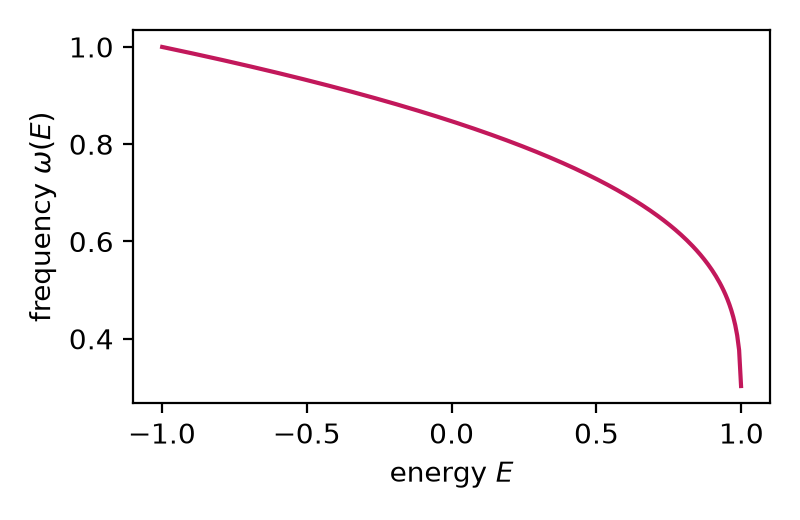
\includegraphics[width=0.42\linewidth]{figures/ch06-pendulum-omega.png}
\caption{Output of \file{ch06_koopman.py}: the pendulum frequency $\omega(E)$ of
\cref{prop:ko-pendulum}, from $1$ at the bottom to $0$ at the separatrix. Each energy level carries its own
pair of eigenvalues $\pm i\omega(E)$: a continuum.}\label{fig:ko-omega}
\end{nfigure}

\paragraph{Parametrized autoencoders.} A Koopman autoencoder whose middle matrix has fixed eigenvalues $\pm i\omega$
cannot represent this; it would need all harmonics $\pm i\omega,\pm2i\omega,\dots$ and a big latent layer
\ts{6}{4}{6:35}\ts{6}{4}{6:55}\ts{6}{4}{7:16}\ts{6}{4}{7:37}\ts{6}{4}{7:57}. Bethany Lusch added an auxiliary network that
learns $\omega$ as a function of the state (in effect of the energy), keeping a $2\times2$ Jordan-block structure
with eigenvalues $\pm i\omega$ \ts{6}{4}{8:17}\ts{6}{4}{8:38}\ts{6}{4}{8:59}. The learned eigenfunctions map the
pendulum to perfect sines and cosines whose frequency depends on the amplitude \ts{6}{4}{9:20}\ts{6}{4}{9:41};
in magnitude and phase they are the action-angle coordinates of classical mechanics, as Mezi\'c pointed out
\ts{6}{4}{10:01}\ts{6}{4}{10:21}. It scales to the cylinder wake \ts{6}{4}{10:42}\ts{6}{4}{11:03}.

\begin{intuition}[Action-angle variables are Koopman eigenfunctions]
For an integrable system with actions $I$ and angles $\vartheta$, $\dot I=0$ and $\dot\vartheta=\omega(I)$. So any
function of $I$ is an eigenfunction with $\lambda=0$, and $h(I)e^{i\vartheta}$ satisfies
$\frac{\mathrm d}{\mathrm dt}=i\omega(I)\,h(I)e^{i\vartheta}$: an eigenfunction only on each torus, with an
eigenvalue that depends on the torus. That is the continuous spectrum, and it is why the auxiliary network
must output $\omega(I)$.
\end{intuition}

Continuous spectra are ubiquitous: most systems of interest have eigenvalues that deform continuously with
energy or control inputs \ts{6}{4}{11:24}\ts{6}{4}{11:44}. The two leading tools are delay coordinates and deep
(parametrized) autoencoders \ts{6}{4}{12:04}\ts{6}{4}{12:25}.

\paragraph{Multiscale systems.} Kathleen Champion: DMD on delay coordinates gives nearly perfect closed linear
models of quasi-periodic van der Pol, Lorenz and R\"ossler oscillators, improving with the rank and the delay
\ts{6}{5}{1:04}\ts{6}{5}{1:25}\ts{6}{5}{1:46}; with a slow and a fast van der Pol oscillator coupled, it separates the
time scales from the single measurement $x_1+x_2$ \ts{6}{5}{2:06}\ts{6}{5}{2:27}. Kutz's multiresolution DMD pulls
out intermittent phenomena such as El Ni\~no from sea-surface temperature \ts{6}{5}{2:27}\ts{6}{5}{2:48}.
Summary: regression methods (DMD, EDMD, sparse eigenfunctions, networks) find coordinates in which a nonlinear
system is linear; the coordinates are a one-time cost that pays off downstream in control; open questions are
scaling, where it works, and whether the up-front cost is worth it \ts{6}{5}{3:08}\ts{6}{5}{3:29}\ts{6}{5}{4:10}.

\begin{keyformulas}
\begin{itemize}
  \item $\K g=g\circ\vb F$ (linear); generator $\mathcal Lg=\nabla g\cdot\vb f$.
  \item Eigenfunctions $\K\varphi=\mu\varphi$, $\nabla\varphi\cdot\vb f=\lambda\varphi$; products add eigenvalues.
  \item Slow manifold: $(x_1,x_2,x_1^2)$ closes, $K=\begin{psmallmatrix}\mu&0&0\\0&\lambda&-\lambda\\0&0&2\mu\end{psmallmatrix}$;
        $\dot x=x^2$: $\varphi=e^{-1/x}$, $\lambda=1$.
  \item EDMD $K=\Psi'\Psi^\dagger$; cross-validate. Control: $\dot\varphi=\lambda\varphi+\nabla\varphi\cdot B\vb u$.
  \item Pendulum: $\omega(E)=\pi/2K(k)$, continuous spectrum; action-angle variables.
\end{itemize}
\end{keyformulas}

\section*{Exercises}

\begin{exercise}[Koopman operator of a map]
For the linear map $x_{k+1}=ax_k$ find all polynomial eigenfunctions of $\K$ and their eigenvalues. For the
doubling map $x_{k+1}=2x_k\bmod1$ on $[0,1)$, show that $e^{2\pi i\,2^nx}$ is mapped by $\K$ to $e^{2\pi i2^{n+1}x}$:
$\K$ is a shift on Fourier modes, with no eigenfunction other than constants in $L^2$.
\end{exercise}

\begin{exercise}[Laurent series]
Insert $\varphi(x)=\sum_{k=-\infty}^{\infty}c_kx^k$ into \eqref{eq:ko-pde} for $f(x)=x^2$, derive the recursion for
the coefficients, and show that the solution with $\lambda=1$ is $e^{-1/x}$. What are the eigenfunctions for
other $\lambda$?
\end{exercise}

\begin{exercise}[Eigenfunctions of the slow-manifold system]
Verify that $x_2-\frac{\lambda}{\lambda-2\mu}x_1^2$ is an eigenfunction of \eqref{eq:ko-slow}. Find the eigenvectors
of $K$ and relate them to the eigenfunctions. Then run the EDMD part of \file{ch06_koopman.py} with monomials up
to degree 4 and 5: which spurious eigenvalues disappear?
\end{exercise}

\begin{exercise}[Energy as an eigenfunction]
Show that for any Hamiltonian system $H$ is a Koopman eigenfunction with $\lambda=0$, and so is any function of
$H$. Write \eqref{eq:ko-control} for the pendulum with a torque $u$ and derive the energy-pumping law
$u=-k\,\dot\theta\,(H-H^*)$ from $\frac{\mathrm d}{\mathrm dt}\frac12(H-H^*)^2\le0$.
\end{exercise}

\begin{exercise}[Spectrum of a signal]
Compute the power spectrum of $x(t)$ for Lorenz (from \file{ch03_lorenz.py}) and for the pendulum at two energies.
Compare the broadband Lorenz spectrum with the lines of the pendulum. What happens to the pendulum spectrum if
the record is an ensemble over many energies?
\end{exercise}

\end{paracol}

% !TEX root = ../main.tex
\chapter{Koopman Observable Subspaces and Control}\label{ch:koopmancontrol}
\begin{paracol}{2}

\begin{sources}
\begin{tabularx}{\linewidth}{@{}V l L@{}}
\toprule
\textbf{Video} & \textbf{Length} & \textbf{Content}\\
\midrule
\seg{7}{1}{V7.1 Koopman Observable Subspaces \& Finite Linear Representations of Nonlinear Dynamics for Control} & 31:31 & Koopman operator and invariant subspaces; the slow-manifold example; eigenfunctions from left eigenvectors; Koopman operator optimal control; when finite closure including the state is impossible (multiple fixed points); logistic map and $\dot x=x^2$; truncations.\\
\seg{7}{2}{V7.2 Koopman Observable Subspaces \& Nonlinearization} & 4:38 & The 3D picture: initial-condition paraboloid, slow-manifold sheet, slow Koopman subspace.\\
\seg{7}{3}{V7.3 Koopman Operator Optimal Control} & 10:18 & The code: LQR on the linearization versus LQR on the Koopman system; the nonlinear gain; one third of the cost.\\
\bottomrule
\end{tabularx}

\smallskip
\textbf{Transcripts} \file{materials/transcripts/C07-V0*.txt}.
\textbf{Book} Sec.~7.4; Sec.~8.4 (LQR).
\textbf{Paper} S.~L.~Brunton, B.~W.~Brunton, J.~L.~Proctor, J.~N.~Kutz, \emph{Koopman invariant subspaces and finite
linear representations of nonlinear dynamical systems for control}, PLoS ONE 11 (2016) e0150171.
\textbf{Code} \file{code/ch07_koopman_lqr.py}.
\textbf{Order} In the playlist these videos are numbers 17, 19 and 20 (the HAVOK video 18 sits between them).
\end{sources}

\section*{Motivation}
\Cref{ch:koopman} sketched the program; this chapter, built on one paper, asks the precise question: when does a
nonlinear system admit a \emph{finite-dimensional, exact} linear representation that \emph{also contains the
state itself}? When it does, linear optimal control applies verbatim and produces a nonlinear optimal
controller \ts{7}{1}{0:08}\ts{7}{1}{0:30}. The answer is ``rarely'', and the reason is topological.

% ------------------------------------------------------------------
\section{Koopman invariant subspaces that contain the state}\label{sec:kc-subspaces}

Recap \ts{7}{1}{0:51}--\ts{7}{1}{6:45}: for $\dot{\vb x}=\vb f(\vb x)$ with flow map $\vb F_t$, the Koopman operator
$\K_tg=g\circ\vb F_t$ is linear and infinite dimensional; in continuous time $\dot g=\mathcal Kg$ with the
infinitesimal generator. Interest revived with Mezi\'c (2005) and with the 2009--2010 links to fluid data
\ts{7}{1}{1:53}\ts{7}{1}{2:14}.

\paragraph{The picture.} Measure $m$ observables $\vb y=\vb g(\vb x)$ (e.g.\ $x_1$, $x_1^2$, $x_2x_3$). We want a
matrix $K$ with $\vb y_{k+1}=K\vb y_k$ whenever $\vb x_{k+1}=\vb F(\vb x_k)$ \ts{7}{1}{7:06}\ts{7}{1}{7:47}. This is
possible exactly when the span of $\vb g$ is a \emph{Koopman-invariant subspace}; eigenfunctions span such
subspaces, but they are hard to find \ts{7}{1}{8:08}\ts{7}{1}{8:49}\ts{7}{1}{9:09}. For control we also want the state
$\vb x$ itself among the observables, since the cost penalizes $\vb x$ \ts{7}{1}{9:30}\ts{7}{1}{9:50}.

\begin{proposition}[What closure with the state requires]\label{prop:kc-closure}
Let $\vb y=(\vb x,g_{n+1}(\vb x),\dots,g_m(\vb x))$ satisfy $\dot{\vb y}=K\vb y$. Then
\begin{enumerate}[(i)]
  \item every component of $\vb f$ lies in the span of $\vb y$: $\vb f(\vb x)=K_{1:n,:}\,\vb y(\vb x)$;
  \item the derivatives $\nabla g_j\cdot\vb f$ of the added observables lie in the span too
        \ts{7}{1}{21:11}\ts{7}{1}{21:31}\ts{7}{1}{22:12};
  \item the left eigenvectors $\vb c$ of $K$, $\vb c^{\mathsf T}K=\lambda\vb c^{\mathsf T}$, give Koopman
        eigenfunctions $\varphi=\vb c^{\mathsf T}\vb y(\vb x)$ \ts{7}{1}{15:00}.
\end{enumerate}
\end{proposition}
\begin{proof}
(i) and (ii) are the first $n$ and the remaining rows of $\dot{\vb y}=K\vb y$. (iii)
$\dot\varphi=\vb c^{\mathsf T}\dot{\vb y}=\vb c^{\mathsf T}K\vb y=\lambda\vb c^{\mathsf T}\vb y=\lambda\varphi$.
\end{proof}

\begin{casestudy}[The slow-manifold system, again]
For \eqref{eq:ko-slow}, $\vb y=(x_1,x_2,x_1^2)$ closes with
$K=\begin{psmallmatrix}\mu&0&0\\0&\lambda&-\lambda\\0&0&2\mu\end{psmallmatrix}$ \ts{7}{1}{10:31}\ts{7}{1}{11:54}\ts{7}{1}{12:35}\ts{7}{1}{13:17}.
Item (i) is why $x_1^2$ is needed (it appears in $f_2$), item (ii) is the ``lucky'' fact that
$\frac{\mathrm d}{\mathrm dt}x_1^2=2\mu x_1^2$ closes \ts{7}{1}{22:33}. Trajectories of the 3D linear system,
projected on $(y_1,y_2)$, reproduce the nonlinear dynamics exactly \ts{7}{1}{13:38}.
\end{casestudy}

\paragraph{The 3D picture} \ts{7}{2}{1:26}--\ts{7}{2}{4:33}. In $(y_1,y_2,y_3)$:
\begin{itemize}
  \item the \emph{blue} paraboloid $y_3=y_1^2$ is where physical initial conditions must start (the third
        coordinate must equal the square of the first) \ts{7}{2}{2:07}\ts{7}{2}{2:27};
  \item the \emph{red} parabolic sheet $y_2=y_1^2$ is the slow manifold, extended in $y_3$ \ts{7}{2}{2:07};
  \item the \emph{green} plane is the slow subspace of $K$, spanned by the eigenvectors of $\mu$ and $2\mu$;
        white trajectories of the linear system fall quickly onto it and slide to the origin
        \ts{7}{2}{2:48}\ts{7}{2}{3:09}.
\end{itemize}
The green plane does not quite pass through the intersection of red and blue; as $\lambda$ becomes faster it
tilts up until it does \ts{7}{2}{3:30}\ts{7}{2}{3:51}. Indeed the eigenvector of $2\mu$ is
$(0,\,\frac{\lambda}{\lambda-2\mu},\,1)$, so the green plane is $y_2=\frac{\lambda}{\lambda-2\mu}y_3$, which tends to
$y_2=y_3$ for $|\lambda|\gg|\mu|$.

% ------------------------------------------------------------------
\section{Koopman operator optimal control}\label{sec:kc-lqr}

Add a control on $x_2$: $\dot x_2=\lambda(x_2-x_1^2)+u$. The lifted system is
$\dot{\vb y}=K\vb y+Bu$ with $B=(0,1,0)^{\mathsf T}$: same $K$, input only on $y_2$ \ts{7}{1}{16:02}\ts{7}{1}{16:22}.

\begin{definition}[New concepts: LQR]\label{def:kc-lqr}
For $\dot{\vb x}=A\vb x+B\vb u$ the \textbf{linear quadratic regulator} minimizes
$J=\int_0^\infty(\vb x^{\mathsf T}Q\vb x+\vb u^{\mathsf T}R\vb u)\,\mathrm dt$; the optimum is the proportional feedback
$\vb u=-C\vb x$, $C=R^{-1}B^{\mathsf T}P$, where $P$ solves the algebraic Riccati equation
$A^{\mathsf T}P+PA-PBR^{-1}B^{\mathsf T}P+Q=0$. $Q$ weights deviations of the state, $R$ control expenditure
\ts{7}{1}{16:42}\ts{7}{1}{17:03}\ts{7}{3}{3:12}\ts{7}{3}{3:32}. (Named for the linear dynamics and the quadratic cost;
Kalman, 1960.)
\end{definition}

\paragraph{Two controllers} \ts{7}{3}{2:10}--\ts{7}{3}{8:01}:
\begin{enumerate}
  \item \textbf{naive}: linearize at the origin, $A=\begin{psmallmatrix}\mu&0\\0&\lambda\end{psmallmatrix}$, $Q=I$,
        $R=1$, one call to \texttt{lqr}, $u=-C\vb x$ \ts{7}{3}{2:31}\ts{7}{3}{3:53}\ts{7}{3}{4:13};
  \item \textbf{Koopman}: LQR on $(K,B)$ with $Q=\diag(1,1,0)$ (the \emph{same} cost: no penalty on the fictitious
        $y_3$) \ts{7}{3}{5:36}\ts{7}{3}{5:56}. The gain has three entries, so
        \begin{equation}\label{eq:kc-u}
          u=-c_1x_1-c_2x_2-c_3x_1^2 ,
        \end{equation}
        a \emph{nonlinear} feedback obtained from a linear method \ts{7}{1}{17:44}\ts{7}{1}{18:05}\ts{7}{3}{6:57}\ts{7}{3}{7:40}.
\end{enumerate}
In the video the Koopman controller reaches the origin with less deviation and about one third of the total
cost \ts{7}{1}{18:25}\ts{7}{1}{18:46}\ts{7}{3}{8:42}\ts{7}{3}{9:03}\ts{7}{3}{9:23}, and seems to work even from very large
initial conditions, as if globally optimal \ts{7}{3}{9:44}.

\codefile{LQR on the linearization vs on the Koopman system}{../code/ch07_koopman_lqr.py}

With the parameters of the paper, $\mu=-0.1$, $\lambda=1$, $\vb x_0=(-5,5)$, the script prints the gains
$(0,\,2.414)$ and $(0,\,2.414,\,-1.496)$ and total costs $J=4485$ (linearized) and $J=990$ (Koopman), a factor
$\approx4.5$; the exact ratio depends on the initial condition.

\begin{intuition}[Why the extra term helps]
The linearized controller sees only $\dot x_2=\lambda x_2+u$ and fights the term $-\lambda x_1^2$ as an unknown
disturbance. The Koopman controller ``knows'' that $x_2$ is pulled towards $x_1^2$: with $c_3<0$ the feedback
$-c_3x_1^2$ cancels part of $-\lambda x_1^2$, so it cooperates with the slow manifold instead of fighting it
(\cref{sec:ko-control}).
\end{intuition}

% ------------------------------------------------------------------
\section{When finite closure is impossible}\label{sec:kc-limits}

\begin{proposition}[Topological obstruction]\label{prop:kc-topology}
If $\dot{\vb x}=\vb f(\vb x)$ has more than one isolated fixed point, or a periodic orbit, or a more complicated
attractor (e.g.\ Lorenz), it admits no finite-dimensional linear system $\dot{\vb y}=K\vb y$, $\vb y=\vb g(\vb x)$,
with $\vb x$ among the components of $\vb y$ \ts{7}{1}{22:55}\ts{7}{1}{23:15}.
\end{proposition}
\begin{proof}[Sketch (the argument of the paper, not a full proof)]
Since $\vb x$ is a component of $\vb y$, the map $\vb g$ is injective and conjugates the nonlinear flow to the
linear flow restricted to the image $\vb g(M)$, which is invariant. A fixed point $\bar{\vb x}$ maps to a
$\vb y$ with $K\vb y=0$, i.e.\ to $\ker K$, a linear subspace; the fixed points of a linear flow form a connected
set, and the linear flow near $\ker K$ cannot reproduce two separated basins (a rigorous version must handle the
restriction to the curved image $\vb g(M)$); a linear flow has no isolated periodic orbits
(limit cycles) and no strange attractors, since solutions are sums of $e^{\lambda t}$ terms. The video's phrasing:
the flows cannot be topologically conjugate, one cannot be continuously deformed into the other
\ts{7}{1}{23:36}\ts{7}{1}{23:57}.
\end{proof}

This is disappointing but expected: we traded nonlinearity for infinite dimension, and non-trivial dynamics
really uses it \ts{7}{1}{24:18}. There may still be special eigenfunctions spanning finite subspaces, but they will
not include the state \ts{7}{1}{26:43}.

\paragraph{The logistic map.} Try $\vb y_k=(x_k,x_k^2)$ for $x_{k+1}=rx_k(1-x_k)$: already
$x_{k+1}^2=r^2(x_k-x_k^2)^2$ contains $x_k^4$; then $x^8$, and so on: a cascade of complexity
\ts{7}{1}{25:01}\ts{7}{1}{25:42}\ts{7}{1}{26:02}\ts{7}{1}{26:22}. In the monomial basis the rows of $K$ are shifted rows of
Pascal's triangle times powers of $r$ \ts{7}{1}{27:04}: indeed $x_{k+1}^j=r^jx_k^j(1-x_k)^j=r^j\sum_i\binom ji(-1)^ix_k^{j+i}$.
Truncations to $5\times5$ have little predictive value; no good finite approximation was found
\ts{7}{1}{27:45}\ts{7}{1}{28:05}.

\paragraph{$\dot x=x^2$, truncated.} A single fixed point, but finite-time blow-up \ts{7}{1}{28:27}. In the basis
$y_k=x^k$, $\dot y_k=kx^{k-1}\dot x=ky_{k+1}$: $K$ has $1,2,3,\dots$ on the superdiagonal
\ts{7}{1}{28:47}\ts{7}{1}{29:08}. Truncating to $N\times N$ gives better and better approximations as $N$ grows
\ts{7}{1}{29:29}\ts{7}{1}{29:49}\ts{7}{1}{30:10}. The script, for $x_0=0.5$ (blow-up at $t=2$), gives $x(1.8)\approx0.5$,
$0.95$, $1.72$, $2.85$, $4.07$ for $N=1,2,4,8,16$, against the exact $5$: the truncation is the Taylor
polynomial of $x_0/(1-x_0t)$ in $t$, which converges for $t<2$, ever more slowly near the singularity.

\begin{keyformulas}
\begin{itemize}
  \item Closure with the state: $\vb f\in\operatorname{span}\vb y$ and $\nabla g_j\cdot\vb f\in\operatorname{span}\vb y$;
        eigenfunctions from left eigenvectors, $\varphi=\vb c^{\mathsf T}\vb y$.
  \item Koopman LQR: LQR on $(K,B)$, $Q=\diag(1,1,0)$ $\Rightarrow$ $u=-c_1x_1-c_2x_2-c_3x_1^2$.
  \item Obstruction: several fixed points, limit cycles, chaos $\Rightarrow$ no finite closure containing $\vb x$.
\end{itemize}
\end{keyformulas}

\section*{Exercises}

\begin{exercise}[Which systems close?]
Decide whether a finite Koopman-invariant subspace containing the state exists, and find it if so:
(a) $\dot x_1=\mu x_1$, $\dot x_2=\lambda(x_2-x_1^3)$;
(b) $\dot x_1=\mu x_1$, $\dot x_2=\lambda x_2+x_1x_2$;
(c) $\dot x=x-x^3$.
For (b), consider the observable $x_2e^{-x_1/\mu}$.
\end{exercise}

\begin{exercise}[Slow subspace]
Compute the eigenvectors of $K$ for the slow-manifold system and show that the slow (green) subspace is
$y_2=\frac{\lambda}{\lambda-2\mu}y_3$. Plot its intersection with $y_3=y_1^2$ for $\lambda=-1,-10,-100$ ($\mu=-0.1$) and
compare with $y_2=y_1^2$.
\end{exercise}

\begin{exercise}[Cost versus initial condition]
Modify \file{ch07_koopman_lqr.py} to compute the ratio of the two costs on a grid of initial conditions in
$[-5,5]^2$ and plot it. Where does the Koopman controller help most? Does the linearized controller ever fail to
stabilize?
\end{exercise}

\begin{exercise}[Logistic-map Koopman matrix]
Write the first four rows of $K$ in the basis $1,x,x^2,\dots,x^8$ for the logistic map. Truncate to the first
$N$ monomials, iterate from $x_0=0.3$ for $r=2.5$ (a stable fixed point) and $r=3.9$ (chaos), and compare with
the true orbit.
\end{exercise}

\end{paracol}

% !TEX root = ../main.tex
\chapter{Hankel Alternative View of Koopman (HAVOK)}\label{ch:havok}
\begin{paracol}{2}

\begin{sources}
\begin{tabularx}{\linewidth}{@{}V l L@{}}
\toprule
\textbf{Video} & \textbf{Length} & \textbf{Content}\\
\midrule
\seg{8}{1}{V8.1 Hankel Alternative View of Koopman (HAVOK) Analysis [FULL]} & 47:07 & Chaos; Koopman invariant subspaces; Hankel matrix and eigen time-delay coordinates; the Koopman reading of the Hankel matrix; the forced linear model; intermittent forcing and lobe switching; Perron--Frobenius almost-invariant sets; magnetic field and measles; the structure of the model, integer coefficients.\\
\seg{8}{2}{V8.2 Hankel Alternative View of Koopman (HAVOK) Analysis [SHORT]} & 22:41 & The same method in short; choice of $r$ by the optimal hard threshold; only what is new is cited.\\
\seg{8}{3}{V8.3 Magnetic field reversal and Measles outbreaks: HAVOK models of chaos} & 9:39 & The two real-world examples in more detail.\\
\seg{8}{4}{V8.4 Linear model for chaotic Lorenz system [HAVOK]} & 5:27 & The sparse antisymmetric structure of $A$; the integer-coefficient model.\\
\bottomrule
\end{tabularx}

\smallskip
\textbf{Transcripts} \file{materials/transcripts/C08-V0*.txt}.
\textbf{Book} Sec.~7.5 (``Time-delay coordinates'', HAVOK).
\textbf{Paper} S.~L.~Brunton, B.~W.~Brunton, J.~L.~Proctor, E.~Kaiser, J.~N.~Kutz, \emph{Chaos as an intermittently forced
linear system}, Nat.\ Commun.\ 8 (2017) 19.
\textbf{Code} \file{code/ch08_havok.py} (original Matlab code: faculty.washington.edu/sbrunton/HAVOK.zip).
The SHORT video repeats the FULL one: it is cited only where it adds something.
\end{sources}

\section*{Motivation}
The last chapter brings together everything: delay coordinates (\cref{sec:si-extensions}), Koopman invariant subspaces
(\cref{ch:koopmancontrol}), DMD/SINDy regression (\cref{ch:dmd,ch:sindy}) and chaos (\cref{ch:fundamentals}). The result:
a chaotic system, observed through a single time series, is well described as a \emph{linear} system driven by an
\emph{intermittent forcing}, and the forcing announces rare nonlinear events, such as lobe switching in Lorenz, before
they happen \ts{8}{1}{0:02}\ts{8}{1}{0:22}. \Cref{prop:kc-topology} said that no finite linear model containing the state can
reproduce several fixed points; HAVOK sidesteps it by letting a forcing carry the essential nonlinearity.

% ------------------------------------------------------------------
\section{Chaos and the Koopman view}\label{sec:hv-chaos}

Chaotic systems are everywhere: climate, turbulence, the stock market, epidemics, planetary motion \ts{8}{1}{0:44}. Linear
systems have the full toolbox of prediction, estimation and control; nonlinear ones have multiple fixed points (the double
well), periodic orbits, and with more nonlinearity chaos \ts{8}{1}{2:25}\ts{8}{1}{2:46}\ts{8}{1}{3:07}. Two double pendulums
released side by side from nearly the same state stay synchronized for a while, then do completely different acrobatics
\ts{8}{1}{3:48}\ts{8}{1}{4:09}. A cube of initial conditions in Lorenz is stretched and folded ``like taffy'' over the
attractor \ts{8}{1}{4:50}\ts{8}{1}{5:11}\ts{8}{1}{5:32}.

\begin{intuition}[Chaos is not randomness]
The smeared cube is not random: it forms structured, coherent patterns. Chaos balances order and structure against
uncertainty amplification in forward time \ts{8}{1}{5:52}\ts{8}{1}{6:12}\ts{8}{2}{1:05}. That structure is what HAVOK
exploits.
\end{intuition}

Koopman recap: propagate measurements $g(\vb x)$ linearly, at the price of infinite dimension; a Koopman-invariant subspace
gives a matrix, but such subspaces are hard to find \ts{8}{1}{6:53}\ts{8}{1}{7:55}\ts{8}{1}{9:17}\ts{8}{1}{9:58}. HAVOK is an
alternative way to get one for chaotic systems; the acronym ``goes nicely with chaos'' \ts{8}{1}{10:19}\ts{8}{1}{10:41}.

% ------------------------------------------------------------------
\section{Delay coordinates and the Koopman reading of the Hankel matrix}\label{sec:hv-hankel}

\paragraph{Embedding.} Measure only $x(t)$ of Lorenz: it sits on one lobe, switches to the other, unpredictably
\ts{8}{1}{11:23}\ts{8}{1}{11:43}. Build the Hankel matrix \eqref{eq:si-hankel} from time-shifted copies of the series
\ts{8}{1}{12:04}\ts{8}{1}{12:24} and take its SVD, $H=U\Sigma V^*$. The columns of $U$ and $V$ are ordered by singular value: the
first ones are the time series most self-similar to the measurement \ts{8}{1}{12:45}\ts{8}{1}{13:06}\ts{8}{1}{13:27}. The idea is old:
the eigensystem realization algorithm (1985), singular spectrum analysis in climate, and the recent nonlinear Laplacian
spectral analysis of Giannakis and Majda \ts{8}{1}{13:48}\ts{8}{1}{14:09}. Plotting $(v_1,v_2,v_3)$ gives an attractor
diffeomorphic to Lorenz's, by Takens' theorem (\cref{thm:si-takens}); $x$ is a good measurement, $z$ would be a bad one
(it cannot distinguish the two lobes, by the symmetry $(x,y,z)\mapsto(-x,-y,z)$) \ts{8}{1}{14:29}\ts{8}{1}{14:50}\ts{8}{1}{15:11}.

\paragraph{The Koopman reading.} Since $x(t_{k+1})=\K x(t_k)$, the Hankel matrix is a Krylov sequence of the Koopman operator
\ts{8}{1}{15:53}\ts{8}{1}{16:13}\ts{8}{1}{16:33}:
\begin{equation}\label{eq:hv-krylov}
  H=\begin{bmatrix}x(t_1)&x(t_2)&\cdots\\ x(t_2)&x(t_3)&\cdots\\ \vdots&&\end{bmatrix}
   =\begin{bmatrix}x(t_1)&\K x(t_1)&\K^2x(t_1)&\cdots\\ \K x(t_1)&\K^2x(t_1)&\cdots\\ \vdots&&\end{bmatrix}.
\end{equation}
Thousands of columns, but numerically of low rank: for Lorenz the first $r=15$ columns of $U$ express every column of $H$ to
almost machine precision \ts{8}{1}{16:54}\ts{8}{1}{17:15}\ts{8}{1}{17:37}. Each column is $\K$ applied to the previous one, so the
span of the leading columns of $U$ is (approximately) \emph{Koopman invariant}: a data-driven invariant measurement subspace of
eigen time-delay coordinates \ts{8}{1}{17:58}\ts{8}{2}{12:07}\ts{8}{2}{12:27}. In the SHORT video $r=15$ is chosen with the optimal
hard threshold of Gavish and Donoho \ts{8}{2}{18:21}.

\begin{remark}[Why chaos helps]
This works best for chaotic systems: the trajectory never returns exactly and densely explores the attractor, never stuck at
a fixed point or a periodic orbit, so one global model for the attractor makes sense, and more data make the linear dependence
better \ts{8}{1}{18:19}\ts{8}{1}{18:39}\ts{8}{1}{19:00}. It holds for data on the attractor, not for every initial condition
\ts{8}{2}{12:27}.
\end{remark}

\begin{secondary}[Singular values of the Lorenz Hankel matrix]
In \file{ch08_havok.py} ($dt=0.001$, $q=100$ delays, $t\in[0,200]$) the singular values relative to the first are $1$,
$0.15$, $0.02$, $2.4\times10^{-3}$, $2.8\times10^{-4}$, $3\times10^{-5}$, \dots: a geometric decay by roughly a factor 8 each.
For a short window ($q\,dt=0.1$) the delay vector is essentially a Taylor expansion of $x(t)$ around the window, which is why
the modes $u_k$ look like Legendre polynomials (see \cref{sec:hv-structure}) and why the singular values decay geometrically.
\end{secondary}

% ------------------------------------------------------------------
\section{Chaos as an intermittently forced linear system}\label{sec:hv-model}

Regress the time derivatives of the eigen time-delay coordinates on the coordinates themselves, as in DMD or SINDy but on
$\vb v=(v_1,\dots,v_r)$ \ts{8}{1}{19:41}\ts{8}{1}{20:01}\ts{8}{1}{20:22}. The first $r-1$ equations fit very well; the last one, for
$v_r$, fits terribly, even with nonlinear terms \ts{8}{1}{20:43}\ts{8}{1}{21:05}\ts{8}{1}{21:25}\ts{8}{1}{21:46}. So treat $v_r$ as an
external input \ts{8}{1}{22:06}:
\begin{equation}\label{eq:hv-model}
  \frac{\mathrm d}{\mathrm dt}\begin{bmatrix}v_1\\\vdots\\v_{r-1}\end{bmatrix}=A\begin{bmatrix}v_1\\\vdots\\v_{r-1}\end{bmatrix}+B\,v_r(t).
\end{equation}

\begin{definition}[New concepts: HAVOK]\label{def:hv}
The \textbf{Hankel alternative view of Koopman} (HAVOK) model of a scalar time series is \eqref{eq:hv-model}: a linear
system in the first $r-1$ eigen time-delay coordinates, forced by the $r$-th, obtained by least-squares regression. A
\textbf{Hankel} matrix (after Hermann Hankel, 1839--1873) is constant along its anti-diagonals.
\end{definition}

\paragraph{What the model does.} Fed with the measured forcing $v_r$ (in red), the linear model reproduces the dynamics (blue
over the white data) and the attractor; and the forcing bursts exactly when the trajectory switches lobes \ts{8}{1}{22:48}\ts{8}{1}{23:08}\ts{8}{1}{23:29}\ts{8}{1}{23:50}.
Its statistics are strongly non-Gaussian: long tails, rare extreme events driving the switches, as in the work of Sapsis, Majda
and co-workers on intermittency in climate, ocean waves and turbulence \ts{8}{1}{24:10}\ts{8}{1}{24:30}\ts{8}{1}{24:51}.

\codefile{HAVOK on the Lorenz system}{../code/ch08_havok.py}

\begin{nfigure}
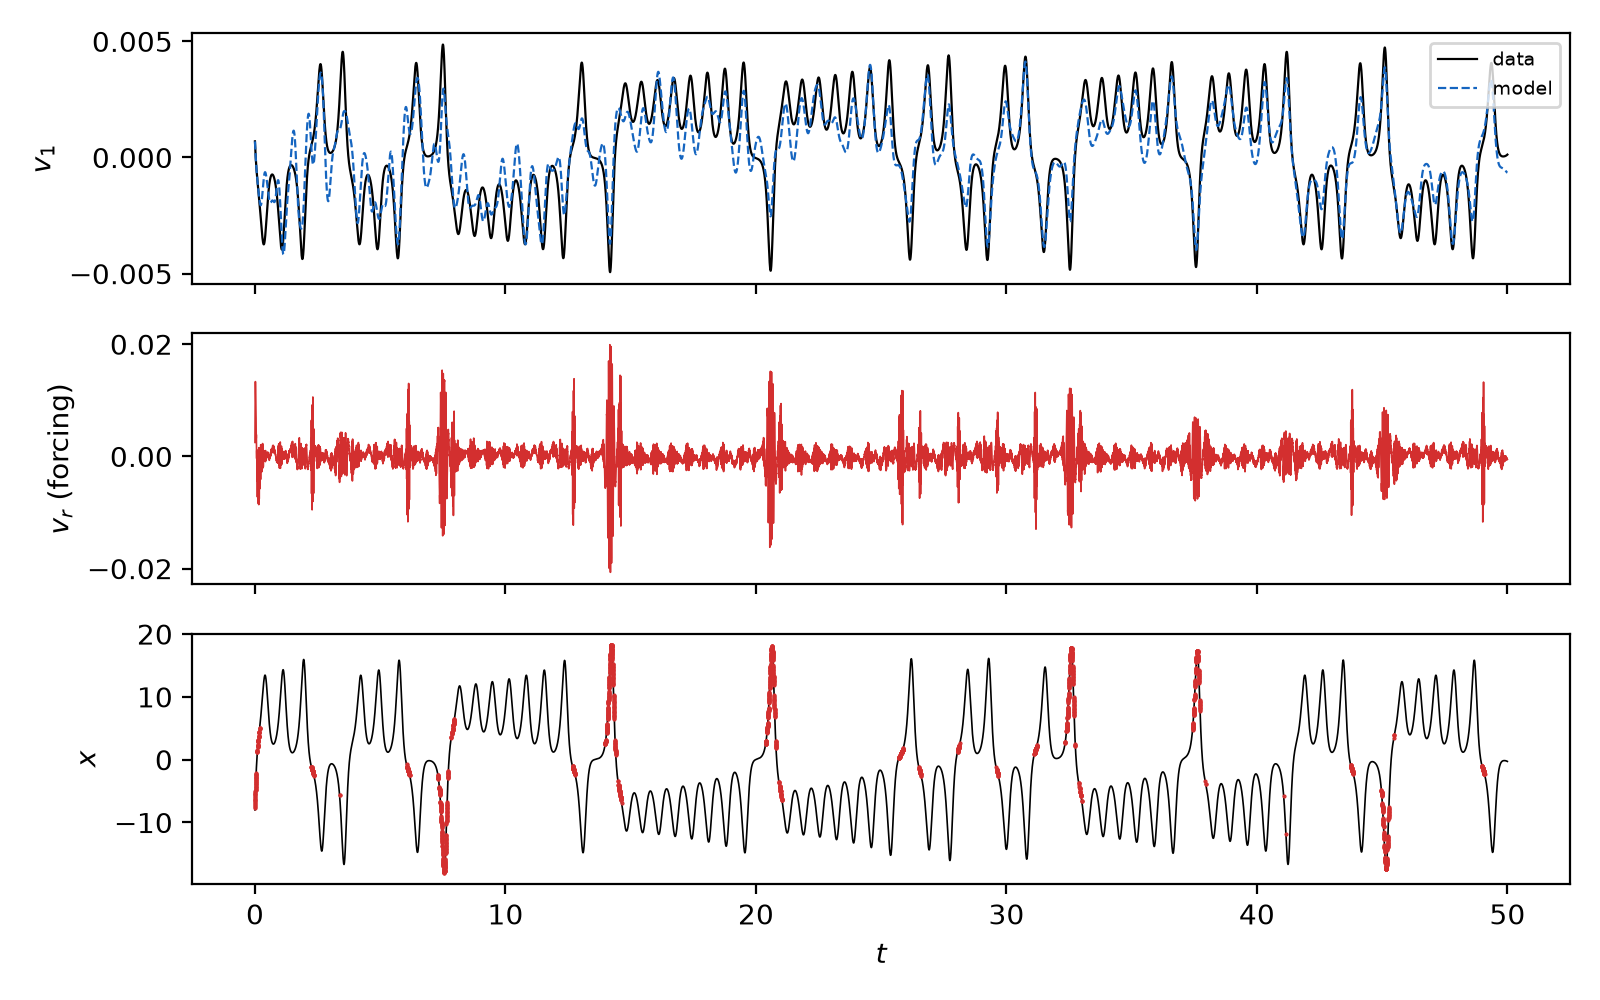
\includegraphics[width=0.78\linewidth]{figures/ch08-havok.png}\hfill
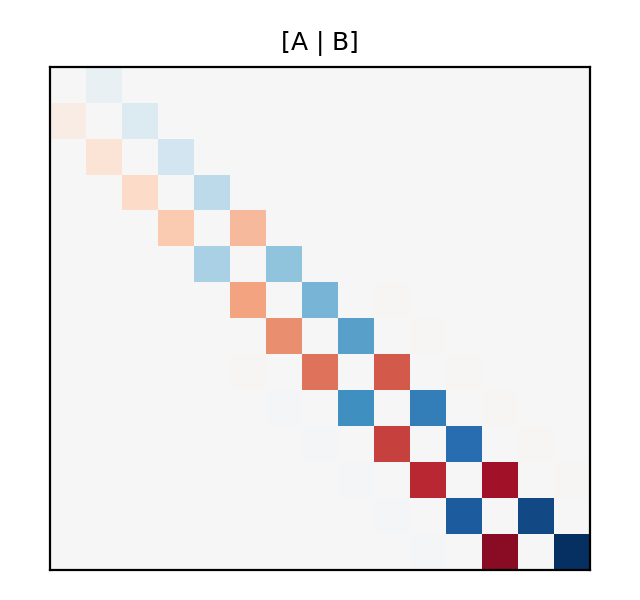
\includegraphics[width=0.2\linewidth]{figures/ch08-havok-A.png}
\caption{Output of \file{ch08_havok.py}. Top: $v_1$ from the data (black) and from the linear model \eqref{eq:hv-model} driven
by the measured forcing (blue dashed); correlation $0.92$ over 50 time units. Middle: the forcing $v_r$, quiet with intermittent
bursts. Bottom: $x(t)$, red where $v_r^2$ exceeds a threshold: the bursts sit at the lobe switches. Right: the matrix $[A\,|\,B]$,
sparse, antisymmetric, nonzero only next to the diagonal.}\label{fig:hv-lorenz}
\end{nfigure}

The script prints a relative residual of $0.97$ for the $v_r$ row, i.e.\ it is not fitted at all, against at most $0.36$ for the
other rows (and much less for the leading ones).

\paragraph{Prediction.} $v_r$ cannot be predicted, but it can be \emph{measured} in real time: project the last window of data
onto the columns of $U$ \ts{8}{1}{27:16}\ts{8}{1}{27:37}. When $v_r^2$ exceeds a threshold, colour the trajectory red: the red flag
rises before the switch, about one revolution ahead \ts{8}{1}{27:57}\ts{8}{1}{28:18}\ts{8}{1}{28:38}\ts{8}{1}{28:59}. It is ``not
perfect'', not every switch is caught \ts{8}{2}{19:23}. On the embedded attractor, white (small forcing) regions are one big
linear Koopman model surrounding the three fixed points; red regions, coherent and not random, mark where essential nonlinearity
acts \ts{8}{1}{29:19}\ts{8}{1}{29:40}\ts{8}{1}{30:01}\ts{8}{1}{30:21}. A typical sequence: four inner revolutions on the right lobe
(white), the flag goes up at point B, one more revolution, switch to the left lobe; there the forcing drops, three revolutions,
flag at D, switch back \ts{8}{1}{33:08}\ts{8}{1}{33:29}\ts{8}{1}{33:49}.

\begin{remark}[Perron--Frobenius almost-invariant sets]
The Perron--Frobenius operator, which advances densities, is dual to Koopman. Its almost-invariant sets for Lorenz are two
interleaved regions (the inner part of one lobe joined to the outer band of the other), and their outer boundaries line up with
the red regions of HAVOK: two very different analyses agree \ts{8}{1}{30:42}\ts{8}{1}{31:02}\ts{8}{1}{31:43}. That the linear part
fails somewhere is unavoidable: a finite linear model has one fixed point, Lorenz has three \ts{8}{1}{32:27}\ts{8}{1}{32:47}.
\end{remark}

% ------------------------------------------------------------------
\section{Real systems: magnetic field reversal and measles}\label{sec:hv-examples}

HAVOK has been applied to R\"ossler, the Mackey--Glass delay equation, the double pendulum, a model of Earth's magnetic field,
electrocardiogram (ECG) and sleep electroencephalogram (EEG) recordings, and measles in New York City; all the code is online
\ts{8}{1}{25:11}\ts{8}{1}{25:32}\ts{8}{1}{25:53}\ts{8}{1}{26:14}.

\begin{casestudy}[Reversals of Earth's magnetic field]
A simulation of averaged magnetohydrodynamic equations, forced by turbulent fluctuations in the Earth's interior, reproduces
geomagnetic reversals \ts{8}{1}{34:30}\ts{8}{1}{34:50}\ts{8}{3}{3:07}. The embedded attractor has two clusters, North pole up and
North pole down, with long stays and sudden jumps; reversals are recorded in the Earth's crust \ts{8}{1}{35:11}\ts{8}{1}{35:31}.
Colouring red where $v_r^2$ exceeds the threshold, the red segments are the reversals \ts{8}{1}{36:12}; there are also near-reversals
that come back \ts{8}{3}{4:10}. Zooming in: just before a flip, $v_1$ is still within its normal fluctuations, and no one could tell
by eye, but the forcing jumps ``clear as day'' \ts{8}{1}{36:53}\ts{8}{1}{37:13}\ts{8}{3}{5:52}. Not 100\%, but a real heads-up
\ts{8}{3}{6:13}.
\end{casestudy}

\begin{casestudy}[Measles in New York City]
Biweekly measles cases in New York, 1928--1964, a classic of delay embedding since Sugihara and May (Nature, 1990)
\ts{8}{1}{37:35}\ts{8}{3}{6:33}. In eigen time-delay coordinates the quiet state is the origin and each outbreak is a burst-and-return
loop; the bigger the loop, the worse the outbreak \ts{8}{1}{37:56}\ts{8}{1}{38:16}. Large outbreaks come with large forcing; the
largest outbreak has the largest forcing event \ts{8}{1}{38:36}. The method ignores small dips in the data that might have been
false alarms and waits for the real precursor \ts{8}{1}{38:57}\ts{8}{3}{7:56}; the first moments of the forcing are already larger
for the worst outbreak, hinting at a prediction of severity \ts{8}{1}{39:18}\ts{8}{3}{8:16}\ts{8}{3}{8:36}.
\end{casestudy}

\begin{history}[Sugihara and May]
George Sugihara and Robert May, \emph{Nonlinear forecasting as a way of distinguishing chaos from measurement error in time
series}, Nature 344 (1990) 734--741, used delay embeddings and nearest-neighbour forecasts on the New York measles and chickenpox
records: measles forecasts degraded with the horizon as for low-dimensional chaos, chickenpox looked like noise around a seasonal
cycle. May is the same ecologist who popularized the logistic map (\cref{sec:si-logistic}).\par
\textit{References:} the paper cited; Brunton et al., Nat.\ Commun.\ 8 (2017).
\end{history}

% ------------------------------------------------------------------
\section{The structure of the HAVOK model}\label{sec:hv-structure}

The Lorenz HAVOK matrix has a striking structure \ts{8}{1}{39:59}\ts{8}{4}{0:44}\ts{8}{4}{1:05}:
\begin{itemize}
  \item \emph{sparse}: nonzero only on the first super- and sub-diagonals \ts{8}{1}{40:20}\ts{8}{1}{41:02};
  \item \emph{antisymmetric}: entries come in equal and opposite pairs \ts{8}{4}{1:25};
  \item the signs on one off-diagonal follow a pattern: four of one sign, then one of the other, three, one, two, one, one
        \ts{8}{1}{41:22}\ts{8}{4}{3:08};
  \item the coefficients are nearly integer multiples of 5: $\pm4.9$, $\pm9.9$, $\pm15.1$, \dots\ \ts{8}{1}{41:43}\ts{8}{4}{2:27}\ts{8}{4}{2:47}.
\end{itemize}
It was discovered by applying SINDy to delay coordinates: even with nonlinear terms allowed, the most parsimonious model was this
sparse linear one, which suggested the connection to Koopman \ts{8}{1}{40:20}\ts{8}{1}{40:41}\ts{8}{4}{1:45}\ts{8}{4}{2:07}. The script
reproduces it: the super-diagonal of $A$ is $-5.18$, $-9.88$, $-13.63$, $-18.76$, $+23.25$, $-28.62$, $-33.47$, $-38.88$: multiples
of 5 (approximately) with a sign flip after the fourth.

\begin{proposition}[Antisymmetric tridiagonal structure from Legendre polynomials]\label{prop:hv-legendre}
If the delay window is short and the modes $u_k$ are (discretized, normalized) Legendre polynomials $P_{k-1}$ on the window, then
the derivative operator in this basis is approximately tridiagonal and antisymmetric, with entries growing linearly with $k$.
\end{proposition}
\begin{proof}[Sketch]
Write $x(t+s)=\sum_kv_k(t)u_k(s)$ for $s$ in the window; then $\dot v_k=\langle u_k,\partial_s x\rangle$, so $A$ is the matrix of
$\partial_s$ in the Legendre basis, truncated. The recurrence $(2n+1)P_n=P_{n+1}'-P_{n-1}'$ makes $\langle P_m,P_n'\rangle$ vanish
unless $m<n$ with $m+n$ odd; a sliding window (data moving through it) symmetrizes this into the antisymmetric part, and the
coefficients scale like $n/\text{window length}$, with nearest neighbours dominating. A precise derivation is in the
literature on HAVOK and on the ``Legendre memory'' of delay embeddings.
\end{proof}

\paragraph{Polynomial modes.} The eigen time series that matter, the columns of $U$, are polynomials for almost all examples:
constant, linear, parabola, cubic, \dots\ \ts{8}{1}{42:25}\ts{8}{1}{42:45}. Convolving a short sliding window of data with this
basis gives the current $v_1,\dots,v_{r-1}$ and the forcing $v_r$ (the 15th, in red) \ts{8}{1}{42:04}\ts{8}{1}{43:05}.

\paragraph{The integer model.} Brunton built a ``neighbouring'' system by hand with exactly this pattern and coefficients
$5,10,15,20,-25,30,35,40,-45,\dots$, and drove it with the $v_{15}$ measured from the real Lorenz system: it shadows the Lorenz
dynamics, lobe switching included, not perfectly but far better than expected; nobody knows why
\ts{8}{1}{43:46}\ts{8}{1}{44:07}\ts{8}{1}{44:27}\ts{8}{1}{44:48}\ts{8}{4}{3:50}\ts{8}{4}{4:32}.

\paragraph{The general lesson.} From data to dynamics \ts{8}{1}{45:09}\ts{8}{1}{45:30}\ts{8}{2}{21:46}:
\begin{enumerate}
  \item measure the right things (embedding theory and observability tell what is a good measurement);
  \item find a representation in which the dynamics is simple: for chaotic systems, eigen time-delay coordinates, a Koopman
        invariant basis in which the dynamics is linear over most of phase space;
  \item regression is the easy part.
\end{enumerate}
Where the forcing is active the system is genuinely nonlinear, but those are exactly the interesting regions: lobe switches,
reversals, outbreaks \ts{8}{1}{46:10}\ts{8}{1}{46:31}.

\begin{keyformulas}
\begin{itemize}
  \item Hankel matrix of $x(t)$ $=$ Krylov sequence $x,\K x,\K^2x,\dots$; $H=U\Sigma V^*$; low rank $\Rightarrow$ leading $u_k$ span an
        approximately Koopman-invariant subspace.
  \item HAVOK: $\dot{\vb v}_{1:r-1}=A\vb v_{1:r-1}+Bv_r$; $v_r$ intermittent, heavy-tailed, active before lobe switches.
  \item $A$: sparse, tridiagonal, antisymmetric, entries $\approx$ multiples of 5 for Lorenz; modes $\approx$ Legendre polynomials.
\end{itemize}
\end{keyformulas}

\section*{Exercises}

\begin{exercise}[Choice of $q$ and $r$]
Run \file{ch08_havok.py} with $q=50,100,200$ and $r=11,15,21$. How do the singular values, the fit residuals and the correlation of
the model change? Use the Gavish--Donoho optimal hard threshold ($\approx2.858\,\sigma_{\text{med}}$ for a square-ish matrix with
unknown noise; for a $q\times m$ matrix use their formula $\omega(\beta)$) to pick $r$ objectively.
\end{exercise}

\begin{exercise}[A bad measurement]
Repeat the analysis with $z(t)$ instead of $x(t)$. Explain, using the symmetry $(x,y,z)\mapsto(-x,-y,z)$, why the embedded attractor
cannot be diffeomorphic to Lorenz and what happens to the forcing.
\end{exercise}

\begin{exercise}[Precursor statistics]
Using the script, define switches as sign changes of $x$ that persist, and red-flag events as upward crossings of the threshold by
$v_r^2$. Compute the fraction of switches preceded by a flag within one revolution and the false-alarm rate, as functions of the
threshold. Remember that $v_r(t_i)$ uses the window $[t_i,t_i+q\,dt]$: shift it to make the forecast causal.
\end{exercise}

\begin{exercise}[Legendre basis]
Plot the first six columns of $U$ against $s\in[0,q\,dt]$ and compare them with the Legendre polynomials $P_0,\dots,P_5$ mapped to the
window. Compute $\langle u_m,\partial_su_n\rangle$ numerically and compare with $A$.
\end{exercise}

\begin{exercise}[Integer model]
Build the antisymmetric tridiagonal matrix with super-diagonal $-5,-10,-15,-20,25,-30,\dots$ (signs as in the script) and drive it with
the measured $v_r$. Compare its $v_1$ with the data and with the fitted HAVOK model.
\end{exercise}

\end{paracol}


\end{document}
